\documentclass[a4paper,11pt,twoside]{report}
\usepackage{booktabs}
\renewcommand{\arraystretch}{1.3}
%-------------------------------------------------------------------------------
%	FONT
%-------------------------------------------------------------------------------
\usepackage[utf8]{inputenc}
\usepackage[T1]{fontenc}
\usepackage{placeins}
%\usepackage[scaled=0.8]{beramono} 

%-------------------------------------------------------------------------------
%	PAGE LAYOUT
%-------------------------------------------------------------------------------
\usepackage[toc,page]{appendix}
\usepackage{titlesec}

\textwidth = 410pt

\usepackage{fancyhdr}
\pagestyle{fancy}
\fancyhf{}

\renewcommand{\sectionmark}[1]{\markright{#1}}

\fancyhead[LO,RE]{Page \thepage}
\fancyhead[LE]{\nouppercase{\leftmark}}
\fancyhead[RO]{\nouppercase{\rightmark}}


\headwidth=1.1\textwidth
\renewcommand{\headrulewidth}{1pt}%{1.5pt}
\renewcommand{\footrulewidth}{0pt}%{1.5pt}
\fancyhfoffset[L]{24pt}
\fancyhfoffset[R]{24pt}

\fancypagestyle{plain}{%
\fancyhf{} % clear all header and footer fields
\headwidth=1.1\textwidth
\renewcommand{\headrulewidth}{1pt}%{1.5pt}
\renewcommand{\footrulewidth}{0pt}
\fancyhead[LO,RE]{Page \thepage}
\fancyhead[LE]{\nouppercase{\leftmark}}
\fancyhead[RO]{\nouppercase{\rightmark}}

\fancyhfoffset[L]{24pt}
\fancyhfoffset[R]{24pt}
}


\newcommand{\mysection}[2]{%
                         \sectionmark{#1}%
                         \section{#2}%
                         \sectionmark{#1}%
                       }

%-------------------------------------------------------------------------------
%	OTHER PACKAGES 
%-------------------------------------------------------------------------------
\usepackage{graphicx}
\usepackage{epstopdf}
\usepackage{subfigure}

\usepackage{float}
\usepackage{tikz}
\usepackage{tikz-uml} 
\usetikzlibrary{trees}
\usepackage{amsmath}

\usepackage{pifont}
\usepackage{fourier}
\usepackage{dingbat}

\usepackage{hyperref}
\usepackage{breakurl}

\usepackage{verbatim}

\usepackage{longtable,tabulary,tabularx}
\usepackage{pdflscape}

\usepackage{multirow}


\usetikzlibrary{matrix,positioning,decorations.pathreplacing,calc}

\newcommand{\ntikzmark}[2]{#2\thinspace\tikz[overlay,remember picture,baseline=(#1.base)]{\node[inner sep=0pt] (#1) {};}}

\newcommand{\makebrace}[3]{%
    \begin{tikzpicture}[overlay, remember picture]
        \draw [decoration={brace,amplitude=0.6em},decorate]
        let \p1=(#1), \p2=(#2) in
        ({max(\x1,\x2)}, {\y1+1.5em}) -- node[right=0.6em] {#3} ({max(\x1,\x2)}, {\y2});
    \end{tikzpicture}
}


%-------------------------------------------------------------------------------
%	TABULARY AND LONGTABLE http://tex.stackexchange.com/questions/78075/multi-page-with-tabulary
%-------------------------------------------------------------------------------
\makeatletter

\def\ltabulary{%
\def\endfirsthead{\\}%
\def\endhead{\\}%
\def\endfoot{\\}%
\def\endlastfoot{\\}%
\def\tabulary{%
  \def\TY@final{%
\def\endfirsthead{\LT@end@hd@ft\LT@firsthead}%
\def\endhead{\LT@end@hd@ft\LT@head}%
\def\endfoot{\LT@end@hd@ft\LT@foot}%
\def\endlastfoot{\LT@end@hd@ft\LT@lastfoot}%
\longtable}%
  \let\endTY@final\endlongtable
  \TY@tabular}%
\dimen@\columnwidth
\advance\dimen@-\LTleft
\advance\dimen@-\LTright
\tabulary\dimen@}

\def\endltabulary{\endtabulary}

\makeatother

%-------------------------------------------------------------------------------
%	CUSTON LISTING SETTINGS
%-------------------------------------------------------------------------------

\usepackage{listings}
\usepackage{lstcustom}
\usepackage{enumerate}
\renewcommand{\lstfontfamily}{\ttfamily}

%-------------------------------------------------------------------------------
%	COLORS
%-------------------------------------------------------------------------------

\definecolor{Lightgray}{gray}{.80}
\definecolor{lightgrey}{rgb}{0.9,0.9,0.9}

%-------------------------------------------------------------------------------
%       Commands
%-------------------------------------------------------------------------------

\newcommand{\reffig}[1]{figure \ref{fig:#1}}
\newcommand{\myparagraph}[1]{\paragraph{#1}\mbox{}\\}

\newcommand{\Code}[1]{\texttt{#1}}
\newcommand{\BornAgain}{\Code{BornAgain}}%
\newcommand{\Python}{\Code{Python}}%
\newcommand{\IsGISAXS}{\Code{IsGISAXS}}%
\newcommand{\SecLabel}[1]{\label{sec:#1}}%
\newcommand{\SecRef}[1]{Section~\ref{sec:#1}}% 
\newcommand{\MakeRemark}[2]
{ \noindent \smallpencil \colorbox{Lightgray}{\parbox{\dimexpr\linewidth-8\fboxsep}			{\underline{#1} #2 }}
}

\newcommand{\ImportantPoint}[2]
{\noindent
  {\huge\danger}\colorbox{Lightgray}{\parbox{\dimexpr\linewidth-8\fboxsep}
 {\underline{#1} #2}}}

\newcommand{\mychapter}[2]{
    \setcounter{chapter}{#1}
    \setcounter{section}{0}
    \chapter*{#2}
    \addcontentsline{toc}{chapter}{#2}
}

\renewcommand\Im{\operatorname{Im}}
\renewcommand\Re{\operatorname{Re}}

\DeclareMathOperator{\sinc}{sinc}

%vector notations
\newcommand{\vect}[1]{\ensuremath{\mathbf{#1}}}
\newcommand{\unitvec}[1]{\ensuremath{\widehat{\vect{#1}}}}
\newcommand{\vectr}{\vect{r}}
\newcommand{\vectk}{\vect{k}}
\newcommand{\vectkt}{\vect{\widetilde{k}}}
\newcommand{\vectq}{\vect{q}}

%curly letters
\newcommand{\curlf}{\ensuremath{\mathcal{F}}}
\newcommand{\curlp}{\ensuremath{\mathcal{P}}}

%basic QM notation (bra, ket, operators, ...)
\newcommand{\oper}[1]{\ensuremath{\mathbf{\hat{#1}}}}
\newcommand{\bra}[1]{\ensuremath{\langle #1 \vert}}
\newcommand{\ket}[1]{\ensuremath{\vert #1 \rangle}}
\newcommand{\braket}[3]{\ensuremath{\left\langle #1 \vert #2 \vert #3 \right\rangle}}
\newcommand{\braketnoop}[2]{\ensuremath{\left\langle #1 \vert #2 \right\rangle}}

%pair correlation functions
\newcommand{\ppcf}[3]{\ensuremath{\mathcal{G}_{#1 ,#2}\left( \vect{#3}_{#1} , \vect{#3}_{#2} \right)}}
\newcommand{\ppcfb}[3]{\ensuremath{\mathcal{G}_{#1 #2}\left( \vect{#3}_{#1 #2} \right)}}

%ensemble average
\newcommand{\ensavg}[2]{\ensuremath{\left\langle #2 \right\rangle_{#1} }}

%reference to equations
\newcommand{\refeq}[1]{equation (\ref{eq:#1})}

%-------------------------------------------------------------------------------
%	TITLE PAGE
%-------------------------------------------------------------------------------
% User Manual version number
% this file is automatically generated by CMakeLists.txt using cmake/modules/UserManualVersion.tex.in

\newcommand{\UserManualVersionNumber}{0.3.1}

 % defines command UserManualVersionNumber
\title{
{\Huge\bf BornAgain}\\[10mm]
Software for simulating and fitting\\
X-ray and neutron small-angle scattering\\
at grazing incidence\\
\vspace*{10mm} User Manual \\
\large{\UserManualVersionNumber} \\
\large{\today}
\vspace*{5mm}
}

\author{ 
{\Large{Céline Durniak, Marina Ganeva, Gennady Pospelov,} }\\
{\Large{Walter Van Herck, Joachim Wuttke} }\\[10mm]
\large
Scientific Computing Group\\
J\"ulich Centre for Neutron Science\\
outstation at Heinz Maier-Leibnitz Zentrum Garching\\
Forschungszentrum J\"ulich GmbH \\ [40mm]
%\normalsize
%Creative Commons CC-BY-SA
}


\date{{}}
\setlength{\headheight}{15pt}
%------------------------------------------------------------------------------
%	DOCUMENT
%------------------------------------------------------------------------------
\begin{document}

\maketitle

\newpage

{\Huge 
\vspace*{0.5cm}
\noindent
Disclaimer
} \newline
\vspace*{0.25cm}

\noindent
{\large
This manual is under development and is not currently a comprehensive listing of
\BornAgain\ features. 
The included information and instructions are a subject to substantial change and
are provided only as a preview.
}

\tableofcontents
%\lstlistoflistings
%\listoffigures
%\listoftables

%%%%%%%%%%%%%%%%%%%%%%%%%%%%%%%%%%%%%%%%%%%%%%%%%%%%%%%%%%%%%%%%%%%%%%%%%%%%%%%%
%%
%%   BornAgain User Manual
%%
%%   homepage:   http://www.bornagainproject.org
%%
%%   copyright:  Forschungszentrum Jülich GmbH 2015
%%
%%   license:    Creative Commons CC-BY-SA
%%   
%%   authors:    Scientific Computing Group at MLZ Garching
%%               C. Durniak, M. Ganeva, G. Pospelov, W. Van Herck, J. Wuttke
%%
%%%%%%%%%%%%%%%%%%%%%%%%%%%%%%%%%%%%%%%%%%%%%%%%%%%%%%%%%%%%%%%%%%%%%%%%%%%%%%%%


\cleardoublepage
\mychapter{0}{Introduction}

\BornAgain\
%\marginpar{scope}%
is a free and open-source software package
to simulate and fit small-angle
scattering at grazing incidence (GISAS)
with X-rays (GISAXS) or neutrons (GISANS).
It provides a generic framework
for modeling multilayer samples with smooth or
rough interfaces and with various types of embedded nanoparticles.
%\marginpar{name}%
The name, \BornAgain,
alludes to the central role of the distorted-wave Born
approximation (DWBA) in the physical description of the
scattering process.
\index{Distorted-wave Born approximation}

\BornAgain\
%\marginpar{extends \IsGISAXS}
almost completely reproduces the functionality
of the widely used program \IsGISAXS\
\index{IsGISAXS@\IsGISAXS}
\index{Lazzari, R\'emi}
by R\'emi Lazzari \cite{Laz02,Laz08}.
\BornAgain\ goes beyond \IsGISAXS\ by
supporting an unrestricted number of layers and particles, 
diffuse reflection from rough layer interfaces,
particles with inner structures, neutron polarization and magnetic scattering.
Adhering to a strict object-oriented design,
\BornAgain\ provides a solid base for future extensions
in response to specific user needs.

\BornAgain\
%\marginpar{platforms}%
\index{Platform|see {Operating system}}%
\index{Operating system}%
is operating system independent.
We actively support
Linux,
\index{Linux}%
MacOS
\index{MacOS}%
and  Microsoft Windows.
\index{Windows|see {Microsoft Windows}}%
\index{Microsoft Windows}%
%\marginpar{licence}%
It is a free and open source software under
the GNU General Public License (GPL, version 3 or higher).
This documentation is released under the Creative Commons license CC-BY-SA.
When \BornAgain\ is used in preparing scientific papers,
please cite software and manual as follows:
\index{Citation}%
%\marginpar{citation}%
\begin{quote}
C.~Durniak, M.~Ganeva, G.~Pospelov, W.~Van Herck, J.~Wuttke (2015),\newline
BornAgain --- Software for simulating and fitting
X-ray and neutron small-angle scattering at grazing incidence,
version \UserManualVersionNumber,\newline
\url{http://www.bornagainproject.org}
\end{quote}

This User Manual is complementary to the online documentation
at \url{http://www.bornagainproject.org}.
It does not duplicate information that is more conveniently read online.
Therefore, Sect.~\ref{sec:online} just contains a few pointers to the web site.
The remainder of this User Manual mostly contains background
on the sample models and on the scattering theory implemented in \BornAgain,
and some documentation of the corresponding \Python\ functions.
%Sect.~\ref{sec:Simulation} describes
%the general methodology of a simulation with \BornAgain,
%and gives detailed usage examples.
%Sect.~\ref{sec:ScatteringCrosssection} explains
%which sample structures are supported in \BornAgain,
%and which physical approximations are used.
%Fitting is explained in Sect.~\ref{sec:Fitting}.
%More theoretical background is given in Appendix~\ref{app:theory}.
%Implemented particle formfactors are specified in Appendix~\ref{app:ff}.

\Warn{\indent Software and documentation are work in progress.
We cannot guarantee that they are accurate and correct.
Anyway, it is entirely in the responsibility of users
to ensure that their data interpretation is physically meaningful.
If in doubt, please contact us.}

\index{Bug reports}
We are grateful for all kind of feedback:
criticism, praise, bug reports, feature requests or contributed modules.
If questions go beyond normal user support,
we will be glad to discuss a scientific collaboration.

\newpage
\section{Quick start} \SecLabel{QuickStart}

This section shortly describes how to build \BornAgain\ from source and run first
simulation. More details about software architecture and installation
procedure are given in \SecRef{SoftwareArchitecture} and \SecRef{InstallationProcedure}. \\

\noindent
{\bf Step I: $~$ installing third party software}
\begin{itemize}
\item boost library ($\geq 1.48$)
\item GNU scientific library ($\geq 1.15$)
\item fftw3 library ($\geq 3.3.1$)
\item python-2.7, python-devel, python-numpy-devel
\item Eigen3 library ($\geq 3.1.0$), optional
\item ROOT framework ($\geq 5.34.00$), optional
\item python-matplotlib, optional
\end{itemize}
\vspace*{2mm}


\noindent
{\bf Step II: $~$ getting the source}
\begin{lstlisting}[language=bash, style=commandline]
git clone git://apps.jcns.fz-juelich.de/BornAgain.git 
\end{lstlisting}
\vspace*{3mm}


\noindent
{\bf Step III: $~$ building the source}
\begin{lstlisting}[language=shell, style=commandline]
mkdir <build_dir>; cd <build_dir>;
cmake <source_dir> -DCMAKE_INSTALL_PREFIX=<install_dir>
make
make check
make install
\end{lstlisting}
\vspace*{3mm}


\noindent
{\bf Step IV: $~$ running example}
\begin{lstlisting}[language=shell, style=commandline]
cd <install_dir>/Examples/python/ex001_CylindersAndPrisms
python CylindersAndPrisms.py
\end{lstlisting}


%Requirements

%Hardware
%BornAgain is known to work on following platforms:
%Linux (x86, amd64)
%MacOS X (x86)

%Software
%GCC 4.1.2 or above   C/C++ compiler
%or
%clang
%gcc 4.1.2 or above, clang

%\newpage
\section{Installation} \SecLabel{Installation}

This section describes how to build and install \BornAgain\ libraries from the source.
At the moment we support building on x86/x86\_64 Linux and Mac OS X operating systems.
Support for Windows systems is planned in next releases.
%In the later releases we are planing to include support for Windows systems and provide
%binary distributions for major Windows/Mac/Linux.
There are three major steps to building \BornAgain\ :
\begin{enumerate}[1.]
\item Acquire required third-party libraries.
\item Get \BornAgain\ source code.
\item Use \Code{cmake} to build and install software.
\end{enumerate}
The remainder of this section explains each step in detail.

\subsection{Third-party software.}
To successfully build \BornAgain\ a number of prerequisite packages must be installed.

\begin{itemize}
\item compilers: clang  versions $\geq 3.1$ or GCC versions $\geq 4.2$
\item cmake ($\geq 2.8$)
\item boost library ($\geq 1.48$)
\item GNU scientific library ($\geq 1.15$)
\item fftw3 library ($\geq 3.3$)
\item python ($\geq 2.7$), python-devel, python-numpy-devel
\end{itemize}
\vspace*{2mm}

Other packages are optional
\begin{itemize}
\item ROOT framework (adds several additional fitting algorithms to \BornAgain)
\item python-matplotlib (allows to run usage examples with graphics)
%\item Eigen3 library ($\geq 3.1.0$)
\end{itemize}

All required packages can be easily installed on most Linux distributions using the system's package
manager. Below we give a few examples for several selected operation systems. Please note,
that other distributions (Fedora, Mint, etc) may have different commands for invoking the package manager and slightly different names of packages (like ``boost'' instead of ``libboost'' etc). Besides that, the installation should be very similar.
\vspace*{3mm}

% ---------------
%  OpenSuse 12.3
% ---------------
\noindent
{\large\bf OpenSuse 12.3} \newline
Adding ``scientific'' repository 
\begin{lstlisting}[language=shell, style=commandline]
sudo zypper ar http://download.opensuse.org/repositories/science/openSUSE_12.3 science
\end{lstlisting}

\noindent
Installing required packages
\begin{lstlisting}[language=shell, style=commandline]
sudo zypper install git-core cmake gsl-devel boost-devel fftw3-devel python-devel python-numpy-devel
\end{lstlisting}

\noindent
Installing optional packages
\begin{lstlisting}[language=shell, style=commandline]
sudo zypper install libroot-* root-plugin-* root-system-* root-ttf libeigen3-devel python-matplotlib
\end{lstlisting}
\vspace*{3mm}


% ---------------
%  Ubuntu 13.04
% ---------------
\noindent
{\large\bf Ubuntu 13.04} \newline
Installing required packages
\begin{lstlisting}[language=shell, style=commandline]
sudo apt-get install git cmake libgsl0-dev libboost-all-dev libfftw3-dev python-dev python-numpy
\end{lstlisting}

\noindent
Installing optional packages
\begin{lstlisting}[language=shell, style=commandline]
sudo apt-get install libroot-* root-plugin-* root-system-* ttf-root-installer libeigen3-dev python-matplotlib python-matplotlib-tk
\end{lstlisting}
\vspace*{3mm}


% ---------------
%  MacOS 10.8
% ---------------
\noindent
\noindent
{\large\bf Mac OS X 10.8} \newline
To simplify the installation of third party open-source software on a Mac OS X system we recommend the use of \Code{MacPorts} package manager. 
The easiest way to install MacPorts is by downloading the \Code{dmg} 
from \url{www.macports.org/install.php} and running the system's installer.
After the installation new command ``\Code{port}'' will be available in terminal window of your Mac. \

\noindent
Installing required packages
\begin{lstlisting}[language=shell, style=commandline]
sudo port -v selfupdate
sudo port install git-core cmake
sudo port install fftw-3 gsl
sudo port install boost -no_single-no_static+python27 


\end{lstlisting}

\noindent
Installing optional packages
\begin{lstlisting}[language=shell, style=commandline]
sudo port install py27-matplotlib py27-numpy py27-scipy
sudo port install root +fftw3+python27
sudo port install eigen3
\end{lstlisting}




\subsection{Getting source code}
\BornAgain\ source can be downloaded at \url{http://apps.jcns.fz-juelich.de/BornAgain}
and unpacked with
\begin{lstlisting}[language=shell, style=commandline]
tar xfz bornagain-<version>.tgz
\end{lstlisting}

\noindent
Alternatively one can obtain \BornAgain\ source from our public Git repository.
\begin{lstlisting}[language=bash, style=commandline]
git clone git://apps.jcns.fz-juelich.de/BornAgain.git 
\end{lstlisting}
\vspace*{3mm}


\noindent
{\bf\large More about Git} \\
Our Git repository holds two main branches called ``master'' and ``develop''. We consider ``master''
branch to be the main branch where the source code of HEAD always reflects latest stable release. \Code{git clone} command shown above
\begin{enumerate}[1.]
\item gives you a source code snapshot corresponding to the latest stable release,
\item automatically sets up your local master branch to track our remote master branch, 
so you will be able to fetch changes from the remote branch at any time using ``git pull'' command.
\end{enumerate}

Master branch is updating approximately once per month.
% that reflects our release cycle.
The second branch, ``develop'' branch, is a snapshot of the current development.
This is where any automatic nightly builds are built from. The develop branch is
always expected to work, so to get the most recent features one can switch source code to it by
\begin{lstlisting}[language=bash, style=commandline]
cd BornAgain
git checkout develop
git pull
\end{lstlisting}
\vspace*{3mm}



\subsection{Building and installing the code}

\BornAgain\ should be build using \Code{CMake} cross platform build system. 
Having third-party libraries installed on the system and \BornAgain\ source code acquired as was explained in
previous sections, type build commands
\begin{lstlisting}[language=bash, style=commandline]
mkdir <build_dir>
cd <build_dir>
cmake <source_dir> -DCMAKE_INSTALL_PREFIX=<install_dir>
make
\end{lstlisting}
\vspace*{3mm}

Here \Code{<source\_dir>} is the name of directory, where \BornAgain\ source code has been
copied, \Code{<install\_dir>} is the directory, where user wants  the package
to be installed, and \Code{<build\_dir>} is the directory where building will occur.

\MakeRemark{About \Code{CMake}}{
\\Having dedicated directory \Code{<build\_dir>} for build process
is recommended by \Code{CMake}. That allows several builds with different compilers/options from the same source and keeps source directory clean from build remnants. \\
}


Compilation process invoked by the command ``make'' lasts about 10 min for an average laptop
of 2012 edition. On multi-core machines the compilation time  can be decreased by invoking command
``make'' with the parameter ``make -j[N]'', where N is the number of cores.

Running functional tests is an optional but recommended step. Command ``make check''
will compile several additional tests and run them one by one. Every test contains
the simulation of a typical GISAS geometry and the comparison on numerical level of simulation results with reference files. Having 100\% tests passed ensures that your local installation
is correct.
\begin{lstlisting}[language=bash, style=commandline]
make check
...
100% tests passed, 0 tests failed out of 26
Total Test time (real) = 89.19 sec
[100%] Build target check
\end{lstlisting}
\vspace*{3mm}


The last command ``make install'' copies compiled libraries and some usage examples
into  the installation directory.
\begin{lstlisting}[language=bash, style=commandline]
make install
\end{lstlisting}


\subsubsection{Troubleshooting}

In the case of complex system setup, with variety of libraries of different versions 
scattered across multiple places (\Code{/opt/local}, \Code{/usr} etc.),
you may want to help \Code{CMake} to find libraries in proper place. 
In example below
two system variables are defined to force \Code{CMake} to prefer libraries
found in \Code{/opt/local} to other places.
\begin{lstlisting}[language=bash, style=commandline]
export CMAKE_LIBRARY_PATH=/opt/local/lib:$CMAKE_LIBRARY_PATH
export CMAKE_INCLUDE_PATH=/opt/local/include:$CMAKE_INCLUDE_PATH
\end{lstlisting}


If compilation fails for some reason, please submit your bug report including compilation errors
at \url{http://apps.jcns.fz-juelich.de/redmine/projects/bornagain/issues}



\subsection{What is next?}

In your installation directory you will find
\begin{lstlisting}[language=bash, style=commandline]
./include - header files for compilation of your C++ program
./lib - libraries to import into python or link with your C++ program
./Examples - directory with examples
\end{lstlisting}

Run your first example and enjoy first BornAgain simulation plot.
\begin{lstlisting}[language=bash, style=commandline]
cd <install_dir>/Examples/python/ex001_CylindersAndPrisms
python CylindersAndPrisms.py
\end{lstlisting}








\newpage
\chapter{Simulation}  \SecLabel{Simulation}

\section{General methodology}
A simulation of GISAXS using \BornAgain\ consists of following steps:
\begin{itemize}
\item define materials by specifying name and refractive index,
\item define embedded particles by specifying shape, size,
   constituting material, interference function,
\item define layers by specifying thickness, roughness, material,
\item include particles in layers, specifying density, position, orientation, 
\item assemble a multilayered sample,
\item specify input beam and detector characteristics,
\item run the simulation,
\item save the simulated detector image.
\end{itemize}

\noindent
We are planing to organize all these steps in a graphical user interface (GUI).
For the time being, however, \BornAgain\ must be involved via \Code{C++} program or
\Code{Python} scripts. In the following, we describe how to write a 
\Code{Python} script which runs a \BornAgain\ simulation. For tutorials about this programming language, the users are referred to \cite{Lut09}.


More information about the general software architecture and \BornAgain\ internal design are given in \SecRef{SoftwareArchitecture}.


\section{Geometry of the sample}

\noindent The geometry used to describe the sample is shown in \reffig{multil3d}. The $z$-axis is perpendicular to the sample's
surface and pointing upwards. The $x$-axis  is perpendicular to the
detector plane. The input and the
scattered output beams are each characterized by two angles
$\alpha_i$, $\phi_i$ and $\alpha_f$, $\phi_f$, respectively. Our choice of orientation for the
angles $\alpha_i$ and $\alpha_f$ is so that they are positive as shown in \reffig{multil3d}. \\

\begin{figure}[h]
  \centering
    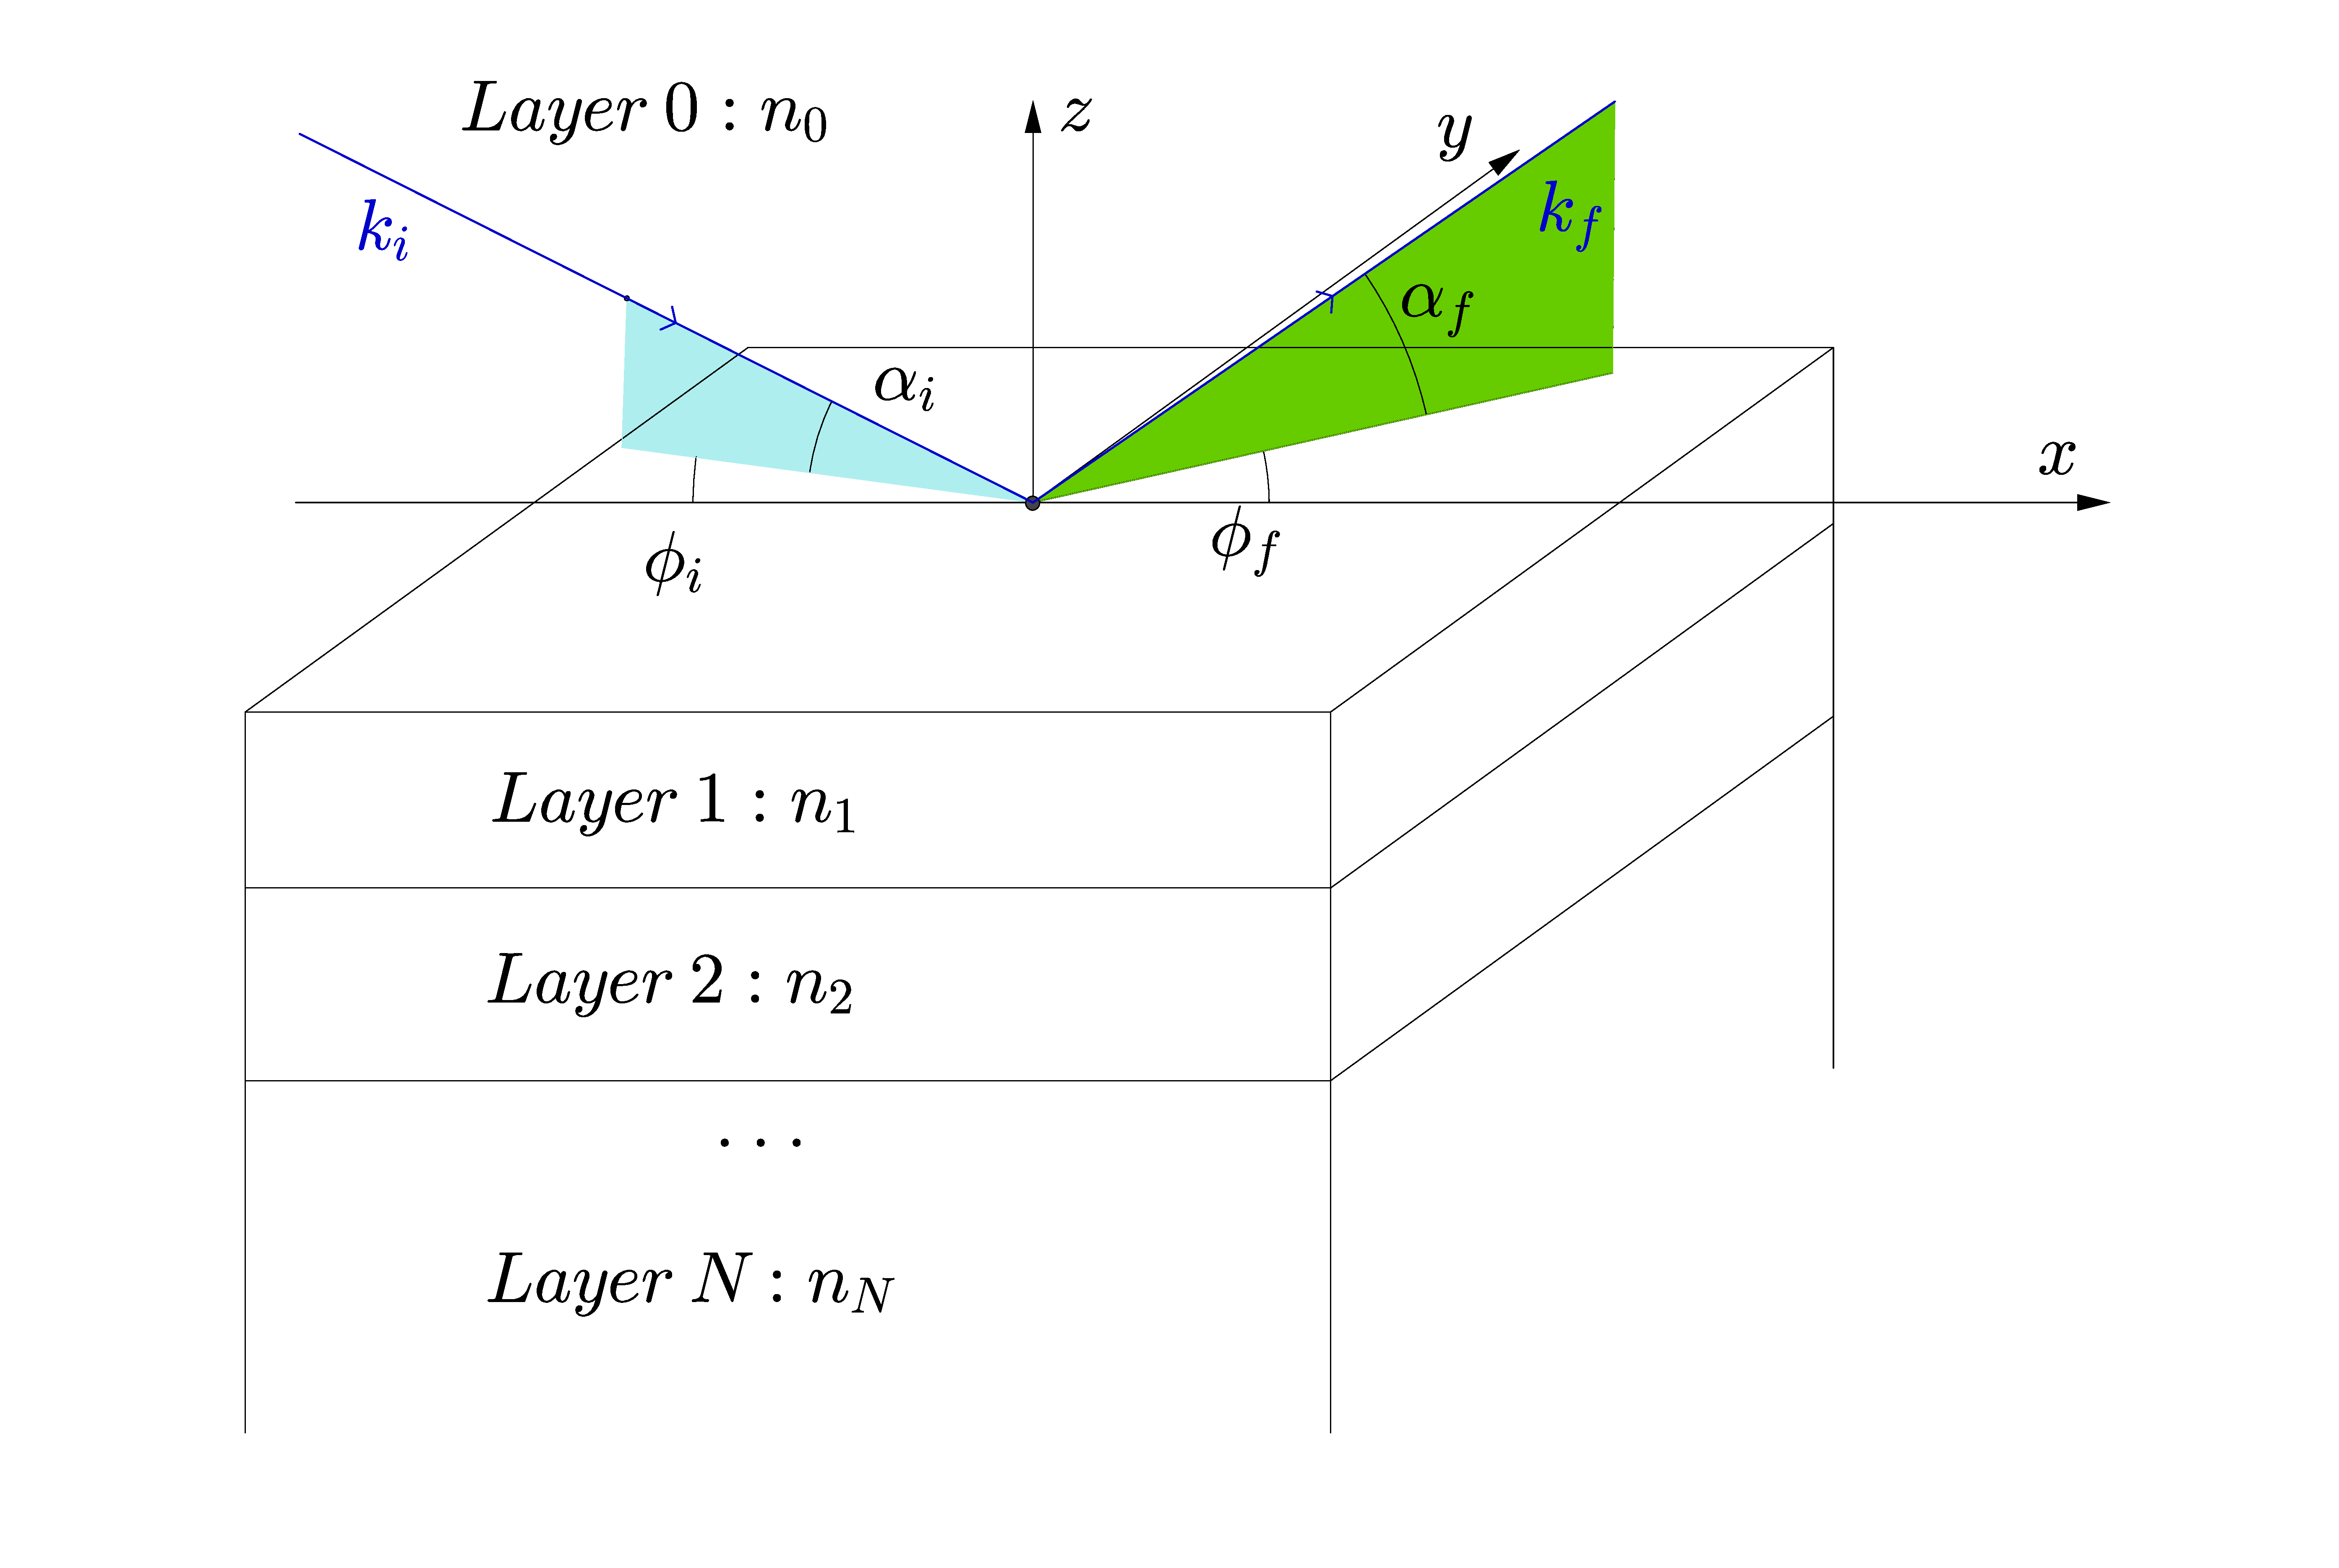
\includegraphics[clip=, width=120mm]{Figures/multilayer3d3.eps}
  \caption[Representation of the scattering geometry.]{Representation of the scattering geometry. $n_j$ is
    the refractive index of layer $j$ and $\alpha_i$ and $\phi_i$ are the incident
    angles of the wave propagating. $\alpha_f$ is the exit angle with respect to the sample's surface and
$\phi_f$ is the scattering angle with respect to the scattering
plane. }
  \label{fig:multil3d}
\end{figure}


The layers are defined by their thicknesses (parallel to the
$z$-direction), their possible
roughnesses (equal to 0 by default) and the
material they are made of. They have infinite extension in the $x$, $y$
directions. And, except for roughness, they interfaces are plane and
perpendicular to the $z$-axis. There is also no limitation to the
number of layers that could be defined in \BornAgain. Note that the
thickness of the top and bottom layer are not defined.

%\ImportantPoint{Remark:}{Order of layers: \\
%When assembling the sample, the layers are defined from top to
%bottom. So in most cases the first layer will be the air layer.}\\

The nanoparticles are characterized by their form factors (\textit{i.e.} the Fourier transform of the shape function - see the list of form factors implemented in \BornAgain) and the composing material. The number of input parameters for the form factor depends on the particle symmetry; it ranges from one parameter for a sphere (its radius) to three for an ellipsoid (its three main axis lengths).
  
By placing the particles
inside or on top of a layer, we impose their vertical positions, whose
values correspond to the bottoms of the particles. The in-plane distribution of particles is linked with the way the
particles interfere with each other. It is therefore implemented
when dealing with the interference function.

%\ImportantPoint{Remark:}{Depth of particles\\
%The vertical positions of particles in a layer are given in relative
%coordinates. For the top layer, the bottom corresponds to
%\texttt{depth}=0. But for all the other layers, it is the top of the
%layer which corresponds to \texttt{depth}=0.}\\

The complex refractive index associated with a layer or a particle is written as $n=1-\delta +i\beta$, with
$\delta, \beta \in \mathbb{R}$. In our program, we input $\delta$ and
$\beta$ directly.


\noindent The input beam is assumed to be monochromatic without any
spatial divergence.\\ %\textbf{polarization term?}

\subsection{Units}
By default the angles are expressed in radians and the lengths are given in
nanometers.  But it is possible to use other units by
specifying them right after the value of the corresponding
parameter like, for example, \Code{20.0*micrometer}.




%%%%%%%%%%%%%%%%%%%%%%%%%%%%%%%%%%%%%%%%%%%%%%%%%%%%%%%%%%%%%%%%%%%%%%%%%%%%%%%%
%%
%%   BornAgain User Manual
%%
%%   homepage:   http://www.bornagainproject.org
%%
%%   copyright:  Forschungszentrum Jülich GmbH 2015
%%
%%   license:    Creative Commons CC-BY-SA
%%   
%%   authors:    Scientific Computing Group at MLZ Garching
%%               C. Durniak, M. Ganeva, G. Pospelov, W. Van Herck, J. Wuttke
%%
%%%%%%%%%%%%%%%%%%%%%%%%%%%%%%%%%%%%%%%%%%%%%%%%%%%%%%%%%%%%%%%%%%%%%%%%%%%%%%%%


\mysection{Example 1: two types of islands on a substrate without interference}{Example 1: two types of islands on top of
  substrate without interference} \SecLabel{Example1Python}

%\section{Example 1: two types of islands on top of
%  substrate without interference.} \SecLabel{Example1Python}

% \sectionmark{Example 1}

In this example, we simulate the scattering from a mixture of
cylindrical and prismatic nanoparticles without any interference
between them. These particles are placed in air, on top
of a substrate.\\ We are going to go through each step of the
simulation. The \Python\ code snippet specific to each stage will be given at
the beginning of the description. 
More examples can be found at our project web site \url{http://www.bornagainproject.org/documentation/python_examples}

% But for the sake of completeness the full code is given
% in Appendix~\ref{PythonSimulationExampleScript}.


% -----------------------------------------------------------------------------
%
% -----------------------------------------------------------------------------
\subsubsection{Importing Python modules}
\begin{lstlisting}[language=python, style=eclipseboxed,name=ex1,nolol]
import numpy @\label{import_lib_beg}@
import matplotlib
import pylab @\label{import_lib_end}@
from bornagain import * @\label{import_ba}@
\end{lstlisting}
We start by importing different functions from external
modules, for example \Code{NumPy} (lines~\ref{import_lib_beg}-\ref{import_lib_end}), which
is a fundamental package for scientific computing with \Python\
\cite{s:numpy}.  In particular, line~\ref{import_ba}
imports the features of \BornAgain\ software.


% -----------------------------------------------------------------------------
%
% -----------------------------------------------------------------------------
\subsubsection{Defining the materials} 
\begin{lstlisting}[language=python, style=eclipseboxed,name=ex1,nolol]
def get_sample(): @\label{def_function}@
    """
    Build and return the sample representing cylinders and pyramids on top of substrate without interference.
   """
    # defining materials @\label{material1}@
    m_air = HomogeneousMaterial("Air", 0.0, 0.0)  @\label{material2}@
    m_substrate = HomogeneousMaterial("Substrate", 6e-6, 2e-8) @\label{material3}@
    m_particle = HomogeneousMaterial("Particle", 6e-4, 2e-8) @\label{materialparticle}@

\end{lstlisting}
Line~\ref{def_function} marks the beginning of the
function to define our sample. Lines~\ref{material2}, \ref{material3} and \ref{materialparticle} define different
materials using class \Code{HomogeneousMaterial}. The general syntax is the following 
\begin{lstlisting}[language=python, style=eclipse,numbers=none]
<material_name> = HomogeneousMaterial("name", delta, beta)
\end{lstlisting}
where \Code{name} is the name of the
material associated with its complex refractive index
n=1-\Code{delta} +i \Code{beta}. \Code{<material\_name>} is later used when
referring to this particular material. The three materials defined in this example are \Code{Air} with a refractive
index of 1 (\Code{delta = beta = 0}), a \Code{Substrate} associated with a complex refractive index
equal to $1-6\times 10^{-6} +i2\times 10^{-8} $, and the material of the particles, whose refractive index is \Code{n}$=1-6\times 10^{-4}+i2\times 10^{-8}$.


% -----------------------------------------------------------------------------
%
% -----------------------------------------------------------------------------
\subsubsection{Defining the particles}
\begin{lstlisting}[language=python,style=eclipseboxed,name=ex1,nolol]
    # collection of particles @\label{particles1}@
    cylinder_ff = FormFactorCylinder(5*nanometer, 5*nanometer) @\label{particlescyl1}@
    cylinder = Particle(m_particle, cylinder_ff) @\label{particlescyl2}@
    prism_ff = FormFactorPrism3(10*nanometer, 5*nanometer) @\label{particlesprism1}@
    prism = Particle(m_particle, prism_ff) @\label{particlesprism2}@
\end{lstlisting}
We implement two different shapes of particles: cylinders and
prisms (\textit{i.e.} elongated particles with a constant equilateral triangular cross section).
 
All particles implemented in \BornAgain\ are defined by their
form factors (see Appendix~\ref{app:ff}), their sizes and the material
they are made of. Here, for the
cylindrical particle, we input its radius and height.  For the prism, 
the possible inputs are the length of one side of its equilateral triangular
base and its height.

In order to define a particle, we proceed in two steps. For example for
the cylindrical particle, we first specify the form factor of a cylinder with 
its radius and height, both equal to 5 nanometers in this particular
case (see line~\ref{particlescyl1}). Then we associate this shape with
the constituting material as in line~\ref{particlescyl2}.
The same procedure has been applied for the prism in lines~\ref{particlesprism1} and \ref{particlesprism2}, respectively.


% -----------------------------------------------------------------------------
%
% -----------------------------------------------------------------------------
\subsubsection{Characterizing particles assembly} 
\begin{lstlisting}[language=python, style=eclipseboxed, name=ex1,nolol]
    particle_layout = ParticleLayout()  @\label{particlesdecor1}@
    particle_layout.addParticle(cylinder, 0.0, 0.5)  @\label{particlesdecor2}@
    particle_layout.addParticle(prism, 0.0, 0.5)@\label{particlesdecor3}@
    interference = InterferenceFunctionNone()  @\label{particlesnointerf}@
    particle_layout.addInterferenceFunction(interference)  @\label{particlesinterf}@
\end{lstlisting}
The object which holds the information about the positions and densities of particles
in our sample is called \Code{ParticleLayout}
(line~\ref{particlesdecor1}). We use the associated function \Code{addParticle}
for each particle shape (lines~\ref{particlesdecor2}, \ref{particlesdecor3}). Its general syntax is 

\begin{lstlisting}[language=python, style=eclipse,numbers=none]
addParticle(<particle_name>, depth, abundance) 
\end{lstlisting}
where \Code{<particle\_name>} is the name used to define the particles
(lines~\ref{particlescyl2} and \ref{particlesprism2}), \Code{depth}
(default value = 0)
is the vertical position, expressed in nanometers, of the particles in a given layer (the
association with a particular layer will be done during the next step) and
\Code{abundance} is the proportion of this type of particles, 
normalized to the total number of particles. Here we have 50\% of cylinders
and 50\% of prisms.

\ImportantPoint{Remark:}{Depth of particles\\
The vertical positions of the particles in a layer are given in relative
coordinates. For the top layer, the bottom of the layer corresponds to
\Code{depth}=0 and negative values would correspond to particles
floating above layer 1 since the vertical axis, shown in \reffig{multil3d} is pointing upwards. But for all the other layers, it is the top of the
layer which corresponds to \Code{depth}=0.}\\


\noindent Finally, lines~\ref{particlesnointerf} and
\ref{particlesinterf} specify that there is \textbf{no coherent interference} between
the waves scattered by these particles. In this case, the intensity is calculated by
the incoherent sum of the scattered waves: $\langle |F_j|^2\rangle$,
where $F_j$ is the form factor associated with the particle of type $j$.  The way these waves
interfere imposes the horizontal distribution of
the particles as
the interference reflects the long or short-range order of the
particles distribution (see  \SecRef{sect:interf}). On the contrary, the vertical position is
imposed when we add the particles in a given layer by parameter \Code{depth}, as shown in lines~\ref{particlesdecor2} and \ref{particlesdecor3}.


% -----------------------------------------------------------------------------
%
% -----------------------------------------------------------------------------
\subsubsection{Multilayer}
\begin{lstlisting}[language=python, style=eclipseboxed,name=ex1,nolol]
# air layer with particles and substrate form multi layer  @\label{sampleassembling}@
    air_layer = Layer(m_air) @\label{airlayer}@
    air_layer.addLayout(particle_layout) @\label{airlayerdecorator}@
    substrate_layer = Layer(m_substrate, 0)  @\label{substratelayer}@
    multi_layer = MultiLayer() @\label{multilayercanvas}@
    multi_layer.addLayer(air_layer) @\label{layerairdecor}@
    multi_layer.addLayer(substrate_layer) @\label{layersubstrate}@
    return multi_layer @\label{returnmlayer}@
\end{lstlisting}
We now have to configure our sample. For this first example,
the particles, \textit{i.e.} cylinders and prisms, are on top of a substrate in an
air layer. \textbf{The order in which we define these layers is important: we
start from the top layer down to the bottom one}.

Let us start with the air layer. It contains the particles. In
line~\ref{airlayer}, we use the previously defined \Code{mAmbience}
(="air" material) (line~\ref{material2}). The command in line~\ref{airlayerdecorator} shows that this layer contains particles
which are defined using particle layout object. The substrate layer
only contains the substrate material (line~\ref{substratelayer}).
%Note that the
%\Code{depth} is referenced to the bottom of the top layer (negative
%values would correspond to particles floating above layer 1 as
%the vertical axis is pointing upwards). 
 
There are different possible syntaxes to define a layer. As shown in
lines~\ref{airlayer} and \ref{substratelayer}, we can use
\Code{Layer(<material\_name>,thickness)} or
\Code{Layer(<material\_name>)}. The second case corresponds
to the default value of the \Code{thickness}, equal to 0. The \Code{thickness} is
expressed in  nanometers.

Our two layers are now fully characterized. The sample is assembled using
\Code{MultiLayer()} constructor (line~\ref{multilayercanvas}): we start with the air layer decorated
with the particles (line~\ref{layerairdecor}), which is the layer at
the top and end with the bottom layer, which is the
substrate (line~\ref{layersubstrate}).


% -----------------------------------------------------------------------------
%
% -----------------------------------------------------------------------------
\subsubsection{Characterizing the input beam and
output detector}

\begin{lstlisting}[language=python, style=eclipseboxed,name=ex1,nolol]
def get_simulation():  @\label{run1}@
    """
    Create and return GISAXS simulation with beam and detector defined
    """
    simulation = Simulation() @\label{run2}@
    simulation.setDetectorParameters(100, -1.0*degree, 1.0*degree, 100, 0.0*degree, 2.0*degree) @\label{rundetector}@
    simulation.setBeamParameters(1.0*angstrom, 0.2*degree, 0.0*degree) @\label{runbeam}@
    return simulation @\label{returnsimul}@
\end{lstlisting}
The first stage is to create the \Code{Simulation()} object (line~\ref{run2}). Then we define the detector (line~\ref{rundetector}) and beam
parameters (line~\ref{runbeam}). %, which are associated with the
%sample previously defined (line~\ref{runsample}). Finally we run
%the simulation (line~\ref{runsimul}). 
Those functions are part of the Simulation
class.  The different incident and exit angles are
shown in \reffig{multil3d}.

The detector parameters are set using ranges of angles via
the function:

\begin{lstlisting}[language=python, style=eclipse,numbers=none]
setDetectorParameters(n_phi, phi_f_min, phi_f_max, n_alpha, alpha_f_min, alpha_f_max),
\end{lstlisting}


\noindent where number of bins \Code{n\_phi}, low edge of first bin \Code{phi\_f\_min} and
upper edge of last bin \Code{phi\_f\_max} all together define $\phi_f$ detector axis, 
while \Code{n\_alpha}, \Code{alpha\_f\_min} and \Code{alpha\_f\_max} are related to 
$\alpha_f$ detector axis.

\ImportantPoint{Remark:}{Axis binning\\
By default axes are binned to provide constant bin size in k-space, which means slightly
non-equidistant binning in angle space. Other possible options, including user defined
axes with custom variable bin size are explained elsewhere.
}
\vspace*{2mm}


%are the minimum and maximum values of $\phi_f$, respectively, \Code{n\_alpha} is
%the number of bins for $\alpha_f$ axis, \Code{alpha\_f\_min} and \Code{alpha\_f\_max} 
%are the minimum and maximum values of
%$\alpha_f$, respectively.

%\Code{isgisaxs\_style=True} (default value = \Code{False}) is a boolean
%used to characterise the structure of the output data. If
%\Code{isgisaxs\_style=True}, the output data is binned at constant
%values of the sine of the output angles, $\alpha_f$ and $\phi_f$, otherwise it is binned
%at constant values of these two angles.\\



\noindent To characterize the beam we use function 
\begin{lstlisting}[language=python, style=eclipse,numbers=none]
setBeamParameters(lambda, alpha_i, phi_i),
\end{lstlisting}

\noindent where \Code{lambda} is the incident beam wavelength,
\Code{alpha\_i} is the incident
grazing angle on the surface of the sample,
\Code{phi\_i} is the in-plane
direction of the incident beam (measured with respect to the $x$-axis).

\ImportantPoint{Remark:}{Scattering vector\\
In \BornAgain\, the wave vector $\mathbf{q}$ is defined as
$\mathbf{k}_i -\mathbf{k}_f$, where $\mathbf{k}_i$ is the incident
wave vector and $\mathbf{k}_f$ the scattered one.}

%\noindent \underline{Remark}: Note that, except for
%\Code{isgisaxs\_style}, there are no default values implemented for the
%parameters of the beam and detector.\\

%\noindent Line~\ref{runsimul} shows the command to run the simulation using the
%previously defined setup.
%%%%%%%%%%%%%


% -----------------------------------------------------------------------------
%
% -----------------------------------------------------------------------------
\subsubsection{Running the simulation  and
  plotting the results}

\begin{lstlisting}[language=python, style=eclipseboxed,name=ex1,nolol]
def run_simulation(): @\label{run_simulation}@
    """
   Run simulation and plot results
    """
    sample = get_sample() @\label{get_sample}@
    simulation = get_simulation() @\label{get_simulation}@
    simulation.setSample(sample)  @\label{setsample}@
    simulation.runSimulation()  @\label{runsimul}@
    result = simulation.getIntensityData().getArray() + 1  # for log scale  @\label{outputdata}@
    pylab.imshow(numpy.rot90(result, 1), norm=matplotlib.colors.LogNorm(), extent=[-1.0, 1.0, 0, 2.0]) @\label{plot1}@
    pylab.show() @\label{plot2}@
\end{lstlisting}
%In function \Code{run\_simulation()}, we associate the sample
%characterised by function \Code{get\_sample()} with the input beam and
%output detector, defined in function \Code{get\_simulation()} (line~\ref{runsample}).
The function, whose definition starts from line~\ref{run_simulation}, gathers all
items. We create the sample and the simulation objects at the lines 
~\ref{get_sample} and \ref{get_simulation}, using calls to the previously defined functions. We assign the sample to the simulation at line ~\ref{setsample} and
finally launch the simulation at line ~\ref{runsimul}.

In line~\ref{outputdata} we obtain the simulated intensity
as a function of outgoing angles $\alpha_f$ and $\phi_f$ for further
uses (plots, fits,\ldots) as a \Code{NumPy} array containing
\Code{n\_phi}$\times$\Code{n\_alpha}
datapoints. Lines~\ref{plot1}-\ref{plot2} produces the two-dimensional
contour plot of the intensity as a function of $\alpha_f$ and
$\phi_f$ shown in \reffig{output_ex1}. 

\begin{figure}[htbp]
  \begin{center}
   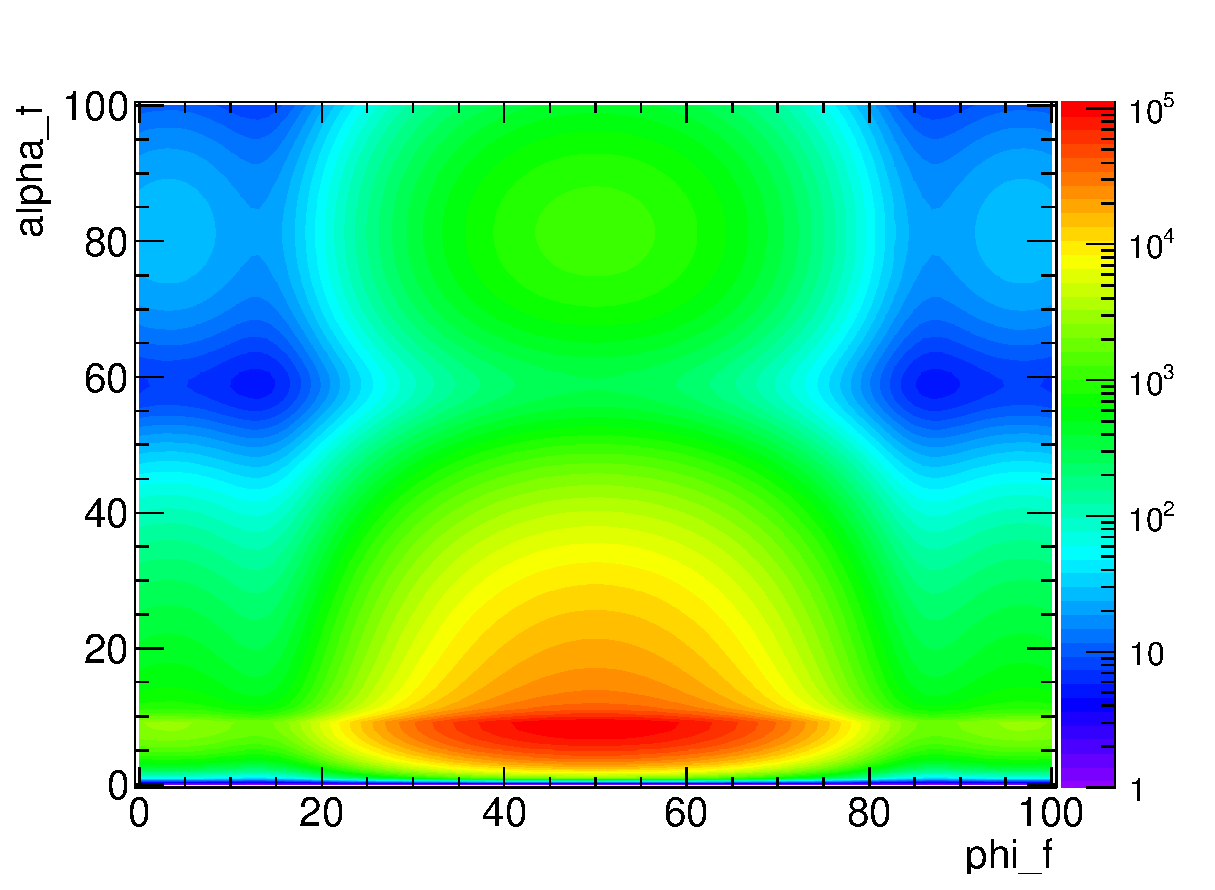
\includegraphics[clip=true, width=120mm]{Figures/gisasmap/Manual_ex1.eps}
  \end{center}
  \caption[Example 1: Simulated grazing-incidence small-angle X-ray scattering from a mixture of
cylindrical and prismatic nanoparticles without any interference, deposited on top
of a substrate]{Simulated grazing-incidence small-angle X-ray scattering from a mixture of
cylindrical and prismatic nanoparticles without any interference, deposited on top
of a substrate. The input beam is characterized by a wavelength
$\lambda$ of 1~\AA\ and incident angles $\alpha_i=0.2^{\circ}$, $\phi_i=0^{\circ}$. The
cylinders have a radius and a height both equal to 5~nm, the prisms
are characterized by a side length equal to 10~nm and they are 5~nm high. The
material of the particles has a refractive index of $1-6\times 10^{-4}+i2\times 10^{-8}$. For the substrate
it is equal to $1-6\times 10^{-6} +i2\times 10^{-8} $. The color scale
is associated with the output intensity in arbitrary units. }
\label{fig:output_ex1}
\end{figure}



%%%%%%%%%%%%%%%%%%%%%%%%%%%%%%%%%%%%%%%%%%%%%%%%%%%%%%%%%%%%%%%%%%%%%%%%%%%%%%%
%
%%%%%%%%%%%%%%%%%%%%%%%%%%%%%%%%%%%%%%%%%%%%%%%%%%%%%%%%%%%%%%%%%%%%%%%%%%%%%%%
\section{Example 2: working with sample parameters} \SecLabel{WorkingWithSampleParameters}

This section gives additional details about the manipulation of sample parameters
during run time; that is after the sample has already been constructed. 
For a single simulation this is normally not necessary. However it might be useful
during interactive work when the user tries to find optimal sample parameters by
running a series of simulations.
A similar task also arises when the theoretical model, composed of the
description of the sample and of the simulation, is used for fitting real data.
In this case, the fitting kernel requires a list of the existing sample parameters
and a mechanism for changing the values of these parameters in order to find 
their optima.

In \BornAgain\ this is done using the so-called sample parameter pool
mechanism. We are going to briefly explain this approach using the example
of \SecRef{Example1Python}.

In \BornAgain\ a sample is described by a hierarchical tree of objects.
For the multilayer created in the previous section this tree can be graphically
represented as shown in Fig.~\ref{fig:sample_tree}. Similar trees can
be printed in a \Python\
session by running \Code{multi\_layer.printSampleTree()}

\begin{figure}[p!]

\tikzstyle{every node}=[draw=black,thick,anchor=west]
\tikzstyle{selected}=[draw=red,fill=red!30]
\tikzstyle{optional}=[dashed,fill=gray!50]
\begin{tikzpicture}[%
  grow via three points={one child at (0.5,-0.7) and
  two children at (0.5,-0.7) and (0.5,-1.4)},
  edge from parent path={(\tikzparentnode.south) |- (\tikzchildnode.west)}]
  \node {MultiLayer}
    child { node {Layer \#0}
		child { node {ParticleLayout } 
			child { node {Particle Info 0} 
				child {node {Particle }  
					child { node {FormFactorCylinder} 
						child { node [optional] { radius:5.0} }					
						child { node [optional] { height:5.0} }					
					}				
				}
    			child [missing] {}		
    			child [missing] {}		
			    child [missing] {}		
				child {node [optional] { abundance:0.5} }			
				child {node [optional] { depth:0.0} }			
			}
    		child [missing] {}		
    		child [missing] {}		
			child [missing] {}		
    		child [missing] {}		
    		child [missing] {}		
			child [missing] {}		
			child { node {Particle Info 1} 
				child {node {Particle }  
					child { node {FormFactorPrism3} 
						child { node [optional] { length:10.0} }					
						child { node [optional] { height:5.0} }					
					}				
				}
    			child [missing] {}		
    			child [missing] {}		
			    child [missing] {}		
				child {node [optional] { abundance:0.5} }			
				child {node [optional] { depth:0.0} }						
			}					
		}
		child [missing] {}		
   		child [missing] {}		
	    child [missing] {}		
		child [missing] {}		
   		child [missing] {}		
	    child [missing] {}		
	    child [missing] {}		
		child [missing] {}		
   		child [missing] {}		
	    child [missing] {}		
		child [missing] {}		
   		child [missing] {}		
	    child [missing] {}		
	    child [missing] {}		
		child {node [optional] { thickness:0.0} }				
    }
	child [missing] {}		
   	child [missing] {}		
	child [missing] {}		
   	child [missing] {}		
	child [missing] {}		
	child [missing] {}		
   	child [missing] {}		
	child [missing] {}		
   	child [missing] {}		
	child [missing] {}		
	child [missing] {}		
   	child [missing] {}		
	child [missing] {}		
   	child [missing] {}		
	child [missing] {}		
	child [missing] {}		
	child { node {Layer interface \#0} 
    	child {node { roughness} 
    		child {node [optional] { corrlength:0.0} }				    	
    		child {node [optional] { hurst:0.0} }				    	
    		child {node [optional] { sigma:0.0} }				    	
    	}					
	}
   	child [missing] {}		
	child [missing] {}		
	child [missing] {}		
    child { node {Layer \#1}
    	child {node [optional] { thickness:0.0} }				
    }
	child [missing] {}		
    child { node [optional] {CrossCorrLength:0.0} };
    
\end{tikzpicture}
\caption{Tree representation of the sample structure.}
\label{fig:sample_tree}
\end{figure}


The top \Code{MultiLayer} object is composed of three children, namely
\Code{Layer \#0, Layer Interface \#0} and \Code{Layer \#1}. The
children objects might themselves also be decomposed into tree-like structures. For example,
\Code{Layer \#0} contains a \Code{ParticleLayout} object, which holds information
related to the two types of particles populating the layer. All numerical values used
during the sample construction (thickness of layers, size of particles, roughness parameters) are part of the same tree structure. 
They are marked in the figure with shaded gray boxes.

These values are registered in the sample parameter pool using the name
composed of the corresponding nodes' names. And they can be accessed/changed
during run time. For example, the \Code{height} of the cylinders
populating the first layer can be changed from the
current value of $5~\rm{nm}$ to $1~\rm{nm}$ by running the command

\begin{lstlisting}[language=shell, style=commandline]
multi_layer.setParameterValue('/MultiLayer/Layer0/ParticleLayout/ParticleInfo0/Particle/FormFactorCylinder/height', 1.0)
\end{lstlisting}


A list of the names and values of all registered sample's parameters
can be displayed using the command 

\begin{lstlisting}[language=shell, style=commandline]
> multi_layer.printParameters()
The sample contains following parameters ('name':value)
'/MultiLayer/Layer0/ParticleLayout/ParticleInfo0/Particle/FormFactorCylinder/height':5
'/MultiLayer/Layer0/ParticleLayout/ParticleInfo0/Particle/FormFactorCylinder/radius':5
'/MultiLayer/Layer0/ParticleLayout/ParticleInfo0/abundance':0.5
'/MultiLayer/Layer0/ParticleLayout/ParticleInfo0/depth':0
'/MultiLayer/Layer0/ParticleLayout/ParticleInfo1/Particle/FormFactorPrism3/length':5
'/MultiLayer/Layer0/ParticleLayout/ParticleInfo1/Particle/FormFactorPrism3/height':5
'/MultiLayer/Layer0/ParticleLayout/ParticleInfo1/abundance':0.5
'/MultiLayer/Layer0/ParticleLayout/ParticleInfo1/depth':0
'/MultiLayer/Layer0/thickness':0
'/MultiLayer/Layer1/thickness':0
'/MultiLayer/LayerInterface/roughness/corrlength':0
'/MultiLayer/LayerInterface/roughness/hurst':0
'/MultiLayer/LayerInterface/roughness/sigma':0
'/MultiLayer/crossCorrLength':0
\end{lstlisting}

Wildcards \Code{'*'} can be used to reduce typing or to work on a group
of parameters. In the example below, the first command will change the
height of all cylinders in the same way, as in the previous example. The second line will change simultaneously the height of {\it both} cylinders and prisms.
\begin{lstlisting}[language=shell, style=commandline]
multi_layer.setParameterValue('*FormFactorCylinder/height', 1.0)
multi_layer.setParameterValue('*height', 1.0)
\end{lstlisting}

The complete example described in this section can be found at 
\begin{lstlisting}[language=shell, style=commandline]
./Examples/python/fitting/ex001_SampleParametersIntro/SampleParametersIntro.py
\end{lstlisting}









\chapter{Scattering cross--section} 

\section{Position of the problem} 
%theoretical description - implementation in \BornAgain
%Influence / contribution of particles (form factor) and sample geometry, interferences between particles, layer roughness,...
%Modelling in grazing incidence : DWBA, BA, level of approximation
%In GISAS experiments, information on the sizes, shapes of the scatterers as well as information on their relative distributions can be obtained.

This section describes how assemblies of particles and layers of materials contribute to the scattering cross--section \textit{i.e.} the way their spatial distributions, the distribution of shapes and their correlations or layers' roughness can influence the output intensity. 

The samples generated with \BornAgain\ are made of different layers of materials characterized by their thicknesses, refractive indices, and possible surface roughnesses. Except for the thickness, the other dimensions of the layers are infinite.\\ Particles can be embedded in or deposited on the top of any layers. Those particles are characterized by their shapes, refractive indices, their spatial distribution and concentration in the sample. The influence of the particles' shapes is described by the form factors. When the particles are densely packed, the distance relative to each other becomes of the same order as the particles' sizes. The radiation scattered from these various particles are going to interfere together. \\ We are first going to give a short overview of the theory involved, mostly in order to define the terminology. For a more complete theoretical description, the user is referred to, for example, reference~\cite{ReLa09} and appendix \ref{appendixtheory} of this manual. Then we are going to describe how the interference features, the form factors and the characteristics of the material layers have been implemented in \BornAgain\ and  give some examples.

%%%%%%%%%%%%%%%%%%%%%%%%%%%%%%%%%%%%%%%%
\section{Collection of particles} \SecLabel{sect:interf}
Let us consider the general geometry of a scattering experiment. An incident neutron with a wave vector $\mathbf{k}_i$ is scattered in a new direction $\mathbf{k}_f$ after interacting with a particle. This scattering occurs in a cone of solid angle $d\Omega$ around the direction of the scattered wave vector $\mathbf{k}_f$.
Considering a set of $N$ particles labeled with index $i$, located at $\mathbf{R}_i$ and having shapes $S_i(\mathbf{r})$ ($S_i=0$ outside the particle and 1 inside), occupying a total volume $V$, the differential cross--section per particle is given by:
\begin{equation*}
  \frac{d\sigma}{d\Omega}(\vect{q}) = \frac{1}{N}\left\lbrace \sum_i \left\lvert F_i(\vect{q}) \right\rvert ^2 + \sum_{i\neq j} F_i(\vect{q}) F_{j}^*(\vect{q}) \exp \left[i\vect{q}\cdot (\vect{R}_i-\vect{R}_j)\right] \right\rbrace \; .
\end{equation*}
where  $\mathbf{q}=\mathbf{k}_i - \mathbf{k}_f$ is the wave vector transfer and $F_i$ is the form factor of particle $i$ (see \SecRef{sect:ff} for a description).


Since in most experimental conditions only the statistical properties of the particles are known, one can consider the probabilistic value of this cross--section \textit{i.e.} its expectation value. Assuming that the particles' shapes are determined by their class $\alpha$, with the abundance ratio $p_\alpha \equiv N_\alpha / N$, and defining the particle density as $\rho_V \equiv N/V$, the expectation value becomes:
\begin{align*}
  \left\langle \frac{d\sigma}{d\Omega}(\vect{q}) \right\rangle  & = \sum_\alpha p_\alpha \left\lvert F_\alpha(\vect{q})\right\rvert ^2 + \frac{\rho_V}{V}\sum_{\alpha,\beta} p_\alpha p_\beta F_\alpha (\vect{q})F_\beta^*(\vect{q})  \\
  & \times \iint_V d^3\vect{R}_\alpha d^3\vect{R}_\beta \ppcf{\alpha}{\beta}{R} \exp \left[ i\vect{q}\cdot (\vect{R}_\alpha - \vect{R}_\beta ) \right] \; ,
\end{align*}

where $\ppcf{\alpha}{\beta}{R}$ is called the \emph{partial pair correlation function}. It represents the normalized probability of finding particles of type $\alpha$ and $\beta$ in positions $\vect{R}_\alpha$ and $\vect{R}_\beta$ respectively. 

%%%%%%%%%%%%%%%%%%%%%%%%%%%%%%%%%%%%%%%%
\subsection{Size-distribution models}

To proceed further, when the morphology and topology are not exactly known, some hypotheses need to be made since the correlation between the kinds of scatterers and their relative positions included in the pair correlation functions are difficult to estimate. Several options are available:

\paragraph{Decoupling approximation (DA)} neglects all correlations. It supposes that the particles are positioned in a way that is completely independent on their kinds (shapes, sizes). An example is given in figure~\ref{fig:da}. Thus the kind of scattering objects and their positions are not correlated and the partial pair correlation function is independent of the particle class $\alpha$. We can therefore replace $ \ppcfb{\alpha}{\beta}{R}$ by  $g(\vect{R}_{\alpha\beta})$.

This leads to the following expression of the scattering cross--section:
\begin{equation*}
\left\langle \frac{d\sigma}{d\Omega}(\vect{q}) \right\rangle  = I_d(\vect{q}) + \left\lvert \left\langle F_\alpha(\vect{q}) \right\rangle_\alpha \right\rvert ^2 \times S(\vect{q}) \; ,
\end{equation*}
where $I_d$ is the diffuse part of the scattering. It is the signature of the fluctuations of shapes, sizes or orientations of the particles; its maximum is located in $q_{\parallel}=0$. In the second term of the expression of the scattering cross-section, $S(\vect{q})$ is the interference function and is given by
\begin{equation*} 
  S(\vect{q}) = 1+ \rho_V \int_V d^3\vect{R} \; g(\vect{R}) \exp \left[ i\vect{q}\cdot \vect{R} \right] \; .
\end{equation*}


\begin{figure}[h]
\begin{center}
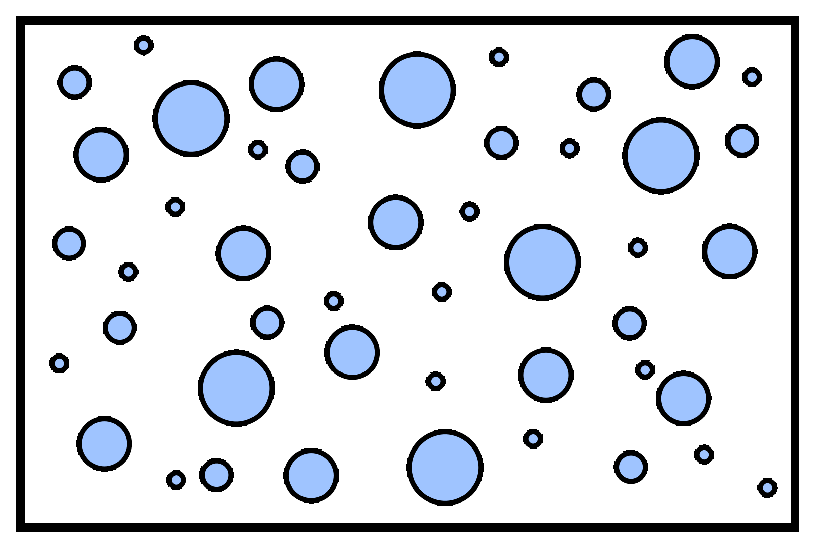
\includegraphics[width=0.5\textwidth]{Figures/drawingDA}
\end{center}
\caption{Sketch of a collection of particles deposited on a substrate whose scattering  could be described by the decoupled approximation.}
\label{fig:da}
\end{figure}


In concentrated systems, DA breaks down because of correlations. One solution is to reintroduce some correlations between particles sizes and distributions using, for example, the size spacing correlation approximation described below. 

\paragraph{Local monodisperse approximation (LMA)} partially accounts for some coupling between the positions and the kinds of the particles \cite{Pede94}. 
 It requires a subdivision of the layers of particles into monodisperse domains. The contributions of these subdomains are then  incoherently summed up and weighted by the size-shape probabilities.\\ In this approximation, a particle is supposed to be surrounded by particles of the same size and shape, within the coherence length of the input beam (see fig.~\ref{fig:lma}). The scattering cross--section is expressed as
\begin{equation*}
  \left\langle \frac{d\sigma}{d\Omega}(\vect{q}) \right\rangle \simeq \left\langle \left\lvert F_\alpha(\vect{q})\right\rvert ^2 S_\alpha(\vect{q}) \right\rangle_\alpha \; .
\end{equation*}

Contrary to the Decoupling Approximation, the Local Monodisperse Approximation can account for particle class/size/shape--dependent pair correlation functions by having distinct interference functions $S_\alpha(\vect{q})$.

One has to remember that in most cases, this approximation corresponds to an unphysical description of the investigated systems. \\ 

DA and LMA separate the contributions of the form factors and of the interference function. For disordered systems DA and LMA give the same result as the scattering vector gets larger \textit{i.e.} the scattered intensity is dominated by the contribution of the form factor.

\begin{figure}[h]
\begin{center}
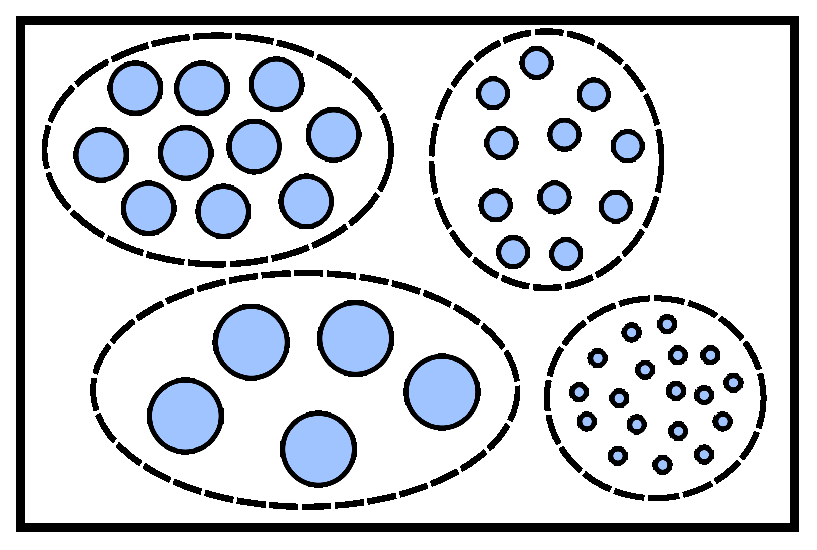
\includegraphics[width=0.5\textwidth]{Figures/drawingLMA}
\end{center}
\caption{Sketch of a collection of particles deposited on a substrate whose scattering could be described by the local monodisperse correlation approximation. The dashed areas mark the coherent domains. In this case, the total scattering intensity is the incoherent sum from all these domains.}
\label{fig:lma}
\end{figure}

\paragraph{Size spacing correlation approximation (SSCA)} introduces correlations between polydisperse particles, more precisely between the shape/size of the particles and their mutual spacing. A classical example would consist of particles whose closest--neighbour spacing depends linearly on the sum of their respective sizes \cite{LaLe07}.

For a sample where only the statistical properties of particle positions and shape/size are known, the scattered intensity per scattering particle is expressed as the average over an ensemble of the Fourier transform of the Patterson function, which is the autocorrelation of the scattering length density $\curlp (\vectr ) \equiv \sum_{ij} S_i(-\vectr )\otimes S_j(\vectr )\otimes \delta (\vectr + \vectr_i - \vectr_j )$:
\begin{equation*}
  I(\vectq ) = \frac{1}{N}\ensavg{}{\curlf (\curlp (\vectr ))} \; ,
\end{equation*}
where $\curlf$ denotes the Fourier transform and $\curlp$ the Patterson function

\begin{figure}[h]
\begin{center}
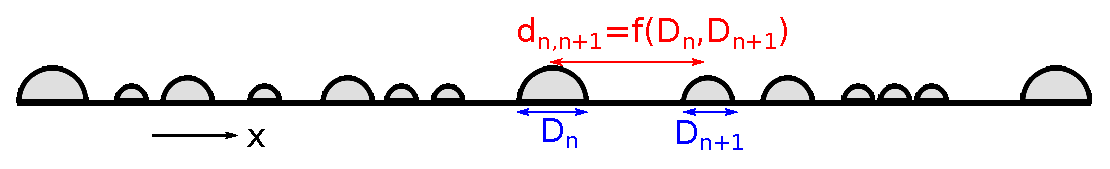
\includegraphics[width=0.9\textwidth]{Figures/drawingSSCA}
\end{center}
\caption{Sketch of a 1D distributed collection of particles, whose scattering could be described by the size-spacing correlation approximation: the distance between two particles depends on their sizes.}
\label{fig:ssca}
\end{figure}

\MakeRemark{Terminology}{
\\
For collections of particles, the scattered intensity contains contributions from neighboring particles. This additional pattern can be called the structure factor, the interference function or even in crystallography, the lattice factor. In this manual, we use the term "interference function" or interferences.
}

%%%%%%%%%%%%%%%%%%%%%%%%%%%%%%%%%%%%%%%%
\subsection{Layout of particles}\label{sec:partlayout}

\subsubsection{The uncorrelated or disordered lattice}
For very diluted distributions of particles, the particles are too far apart from each other to lead to any interference between the waves scattered by each of them. In this case the interference function is equal to 1. The scattered intensity is then entirely determined by the form factors of the particles distributed in the sample.

\subsubsection{The regular  lattice}\mbox{}\\
The particles are positioned at regular intervals generating a layout characterised by its base vectors $\mathbf{a}$ and $\mathbf{b}$ (in direct space) and the angle between these two vectors.
This lattice can be two or one-dimensional depending on the characteristics of the particles. For example when they are infinitely long, the implementation can be simplified and reduced to a "pseudo" 1D system.

\paragraph{The ideal paracrystal} \mbox{}\\
A paracrystal, whose notion  was developed by Hosemann\cite{Hos51}, allows fluctuations of the lengths and orientations of lattice vectors. Paracrystals can be defined as distorted crystals in which the crystalline order has not disappeared and for which the behavior of the interference functions  at small angles is coherent.
It is a transition between the regular lattice and the disordered state.\\


For example, in one dimension, a paracrystal is generated using the following method. First we place a particle at the origin. The second particle is put at a distance $x$ with a density probability $p(x)$ that is peaked at a mean value $D$: $\int_{-\infty} ^{\infty}p(x)dx=1$ and $\int_{-\infty}^{\infty}xp(x)dx=D$. The third one is added at a distance $y$ from the second site using the same rule with a density probability $p_2(y)= \int_{-\infty}^{\infty}p(x)p(y-x)dx=p\otimes p(y)$.\\ With such a method, the pair correlation function $g(x)$ is built step by step. Its expression and the one of its Fourier transform, which is the interference function are 
\begin{equation*}
g(x)=\delta(x)+ p(x)+ p(x)\otimes p(x)+\ldots + p(-x)+\ldots \: \mathrm{and}\:\, S(q)=\Re\left(\dfrac{1+P(q)}{1-P(q)}\right),
\end{equation*}
 where $P(q)$ is the Fourier transform of the density probability $p(x)$.\\


In two dimensions, the paracrystal is constructed on a pseudo-regular lattice with base vectors $\mathbf{a}$ and $\mathbf{b}$ using the following conditions for the densities of probabilities:\\ $\int p_{\mathbf{a}}(\mathbf{r})d^2\mathbf{r}=\int p_{\mathbf{b}}(\mathbf{r})d^2\mathbf{r}=1$, $\int \mathbf{r} p_{\mathbf{a}}(\mathbf{r})d^2\mathbf{r}=\mathbf{a}$, $\int \mathbf{r} p_{\mathbf{b}}(\mathbf{r})d^2\mathbf{r}=\mathbf{b}$.\\
In the ideal case the deformations along the two axes are decoupled and each unit cell should retain a parallelogram shape. The interference function is given by\\ $S(q_{\parallel})=\prod_{k=a,b}\Re\left(\dfrac{1+P_k(q_{\parallel})}{1-P_k(q_{\parallel})} \right)$ with $P_k$ the Fourier transform of $p_k$, $k=a, b$.

\paragraph{Probability distributions} \label{baftd} \mbox{}\\
The scattering by an ordered lattice gives rise to a series of Bragg peaks situated at the nodes of the reciprocal lattice. Any divergence from the ideal crystalline case modifies the output spectrum by, for example, widening or attenuating the Bragg peaks. The influence of these "defects" can be accounted for 
 in direct space using correlation functions or by truncating the lattice or, in reciprocal space with structure factors or interference functions by convoluting the scattered pics with a function which could reproduce the experimental shapes.

%%%%%%%%%%%%%%%%%%%%%%%%%%%%%%%%%%%%%%%%
\subsection{Implementation in \BornAgain}

This section describes the implementation of the interference functions in \BornAgain. For an implementation of all the components of a simulation, the use is referred, for example, to \SecRef{Example1Python}.\\


\ImportantPoint{Remark:}{In \BornAgain\ the particles are positioned in the same vertical layer.}

\subsubsection{Size-distribution models}
The decoupled approximation, local monodisperse approximation and size spacing correlation approximation can be used in \BornAgain.
The selection is made using\\ \Code{SimulationParameters()} when defining the characteristics of the simulation.  For example,
\begin{lstlisting}[language=python, style=eclipseboxed,numbers=none,nolol]
    simulation = Simulation()
   ....
    sim_params = SimulationParameters()
# interference approx chosen between: DA (default), LMA and SSCA
    sim_params.me_if_approx = SimulationParameters.LMA
    simulation.setSimulationParameters(sim_params)
\end{lstlisting}

%The users can refer to Script~\ref{lst:2dlatticeinterf} for a more detailed implementation. By default, the decoupled approximation (DA) is used.

%%%%%%%%%%%%%%%%%%%%%%%%%%%%%%%%%%%%%%%%
\subsubsection{Probability distribution functions}\label{baftd}

The probability distribution functions have been implemented in the reciprocal space in \BornAgain. Their expressions are given in Table~\ref{table:pdf}.

\begin{table}[H]
\centering
\begin{tabular}{ccc}
\hline 
Function & One dimension & Two dimensions\\
\hline 
Cauchy & $(1+q^2\omega^2)^{-3/2}$ & $(1 + q_x^2 cl_x^2 + q_y^2 cl_y^2)^{-3/2}$ \\
Gauss & $\dfrac{1}{2}\exp(-\dfrac{q^2\omega^2}{4})$ & $\frac{1}{2}\exp\left(-\dfrac{q_x^2 cl_x^2+ q_y^2cl_y^2}{4}\right)$ \\
Voigt & $\dfrac{\eta}{2} \exp\left(-\dfrac{q^2\omega^2}{4}\right) + \dfrac{1 - \eta}{(1 + q^2\omega^2)^{3/2}}$ & $\dfrac{\eta}{2} \exp\left(-\dfrac{q_x^2 cl_x^2+ q_y^2cl_y^2}{4}\right)+ \dfrac{1 - \eta}{(1 + q_x^2 cl_x^2+ q_y^2cl_y^2)^{3/2}}$ \\
\hline
\end{tabular}
\caption{List of probability distribution functions in reciprocal space. $\omega$, $cl$ stand for coherence lengths (the index refers to the axis) and  $\eta$ is a weighting coefficient.}
\label{table:pdf}
\end{table}

The Cauchy distribution corresponds to $\exp(-r)$ in real space and the Voigt one  is a linear combination of the Gaussian and Cauchy probability distribution functions.\\

\noindent \underline{One dimension}
\begin{itemize}
\item \Code{FTDistribution1DCauchy($\omega$)},
\item \Code{FTDistribution1DGauss($\omega$)},
\item \Code{FTDistribution1DVoigt($\omega, \eta$)}.
\end{itemize}
where $\omega$ is the coherence length and $\eta$ is a weighting factor.\\

\noindent \underline{Two dimensions}
\begin{itemize}
\item \Code{FTDistribution2DCauchy($cl_x$, $cl_y$)},
\item \Code{FTDistribution2DGauss($cl_x$, $cl_y$)},
\item \Code{FTDistribution2DVoigt($cl_x$, $cl_y$)}
\end{itemize}
where $cl_{x,y}$ are the coherence lengths in the $x$ or $y$ direction, respectively.

These functions can be used with all interference functions except the case without any interference and the one dimensional paracrystal, for which only the Gaussian case has already been implemented.
%%%%%%%%%%%%%%%%%%%%%%%%%%%%%%%%%%%%%%%%
\subsubsection{Interferences}

The interference function is specified when building the sample. It is linked with the particles (shape, material). Examples of implementation are given at the end of each description.

\paragraph{Syntax:}
 \Code{particle\_layout.addInterferenceFunction(interference\_function)},\\ where \Code{particle\_layout} holds the information about the different shapes and their proportions for a given layer of particles, and \Code{interference\_function}  is one of the following expressions:
\begin{itemize}
\item \Code{InterferenceFunctionNone()}
\item \Code{InterferenceFunction1DLattice(lattice\_parameters)}
\item \Code{InterferenceFunction1DParaCrystal(peak\_distance, width,corr\_length)}
\item \Code{InterferenceFunction2DLattice(lattice\_parameters)}
\item \Code{InterferenceFunction2DParaCrystal(length\_1, length\_2, $\alpha$\_lattice, $\xi$, \\ damping\_length)}
\end{itemize}

\ImportantPoint{Remark:}{\Code{InterferenceFunction1DLattice} can only be used for particles which are infinitely long in one direction of the sample's surface like for example a rectangular grating.}

\newpage
%%%%%%%%%%%%%%%%%%%%%%%%%%%%%%%%%%%%%%%%%%
\subsubsection{\ding{253} \Code{InterferenceFunctionNone()}} 
The particles are placed randomly in the dilute limit and are considered as individual, non-interacting scatterers. The scattered intensity is function of the form factors only. 

\paragraph{Example} The sample is made of a substrate on which are deposited half-spheres. Script~\ref{lst:nointerf} details the commands necessary to generate such a sample. Figure~\ref{fig:nointerf} shows an example of output intensity: Script~\ref{lst:nointerf}  + detector's + input beam's characterizations. The full script UMInterferencesNone.py can be found in /Examples/python/UserManual. 


\begin{figure}[h]
\begin{center}
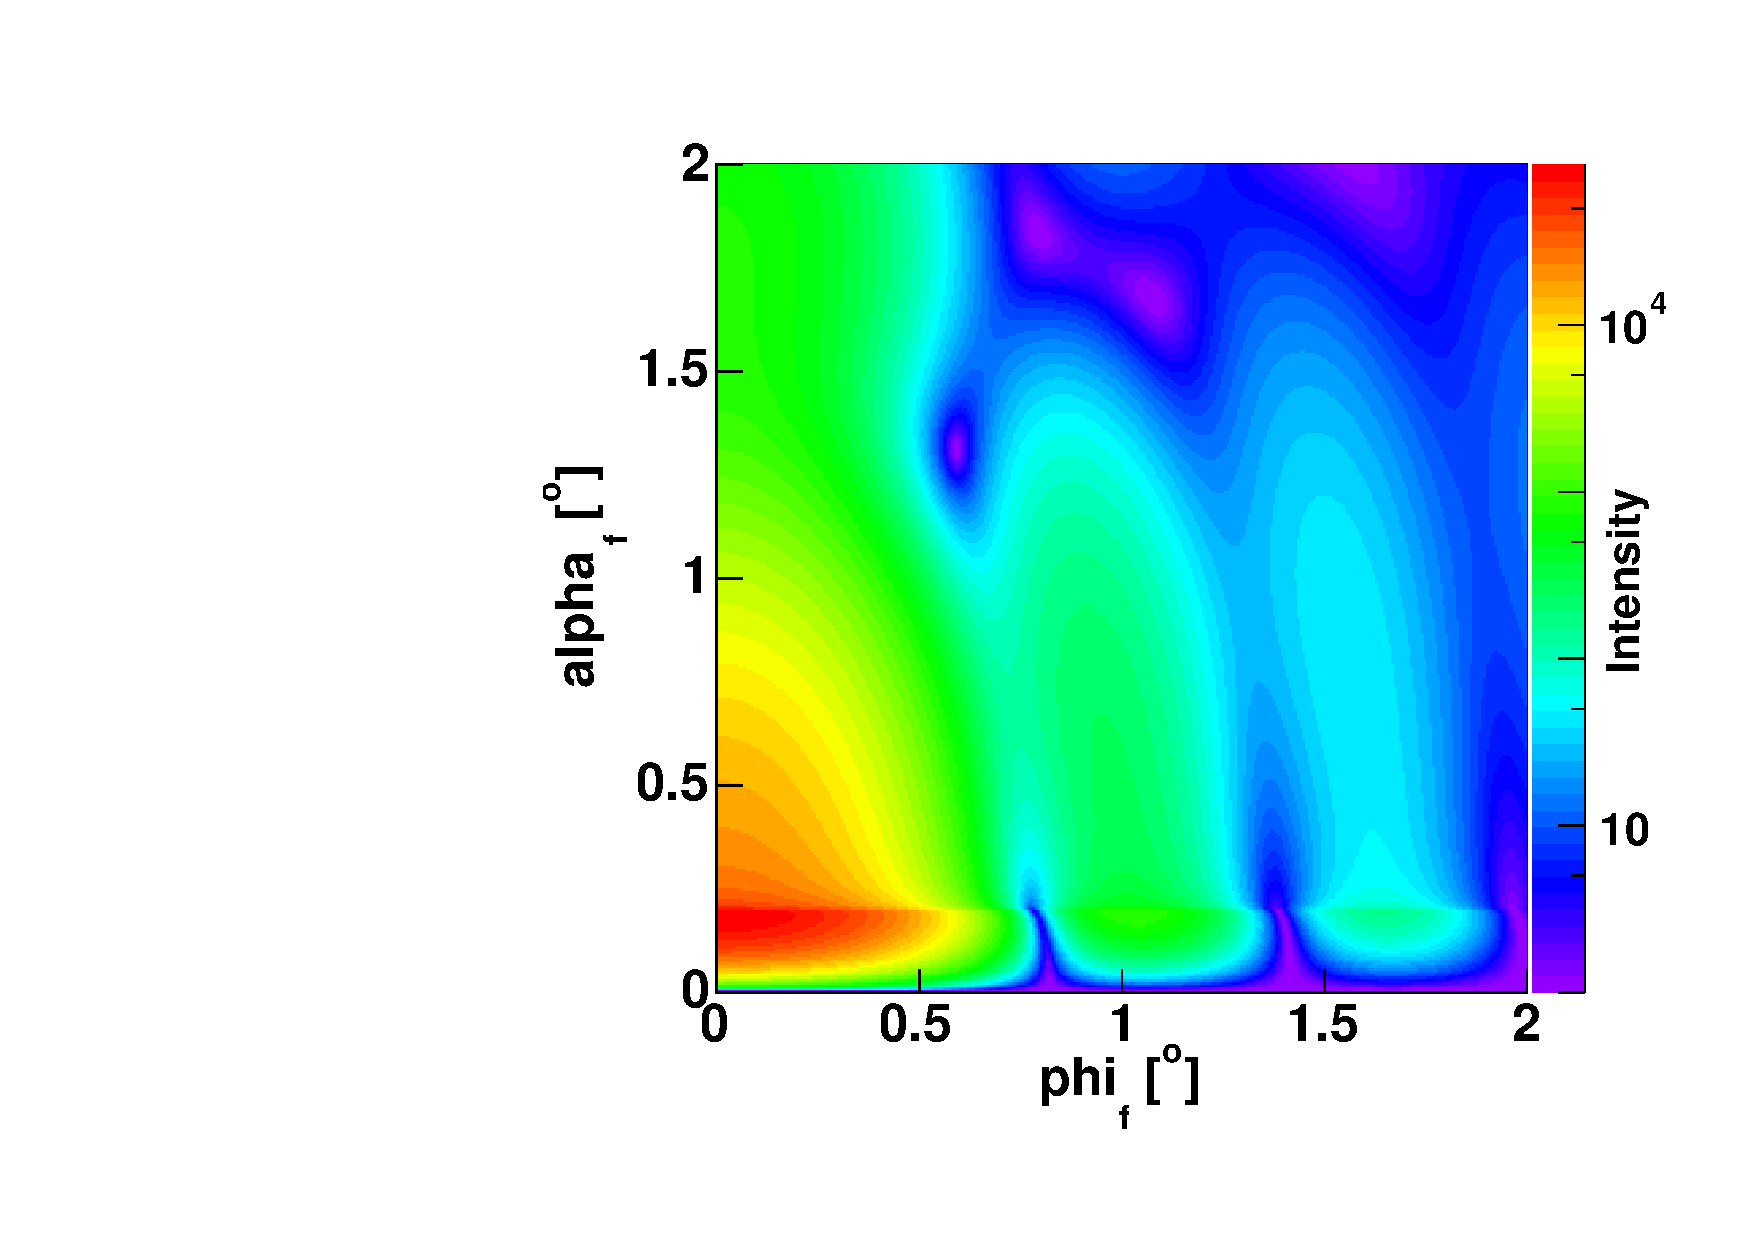
\includegraphics[width=0.5\textwidth]{Figures/HSphere_NoInterf}
\end{center}
\caption{Output intensity scattered from a sample made of half-spheres with no interference between them.}
\label{fig:nointerf}
\end{figure}

\FloatBarrier
\newpage

\begin{lstlisting}[language=python, style=eclipseboxed,numbers=none,nolol,caption={\Code{Python} script to simulate a sample made of half-spheres deposited on a substrate layer without any interference. The part specific to the interferences is marked in red italic font.},label={lst:nointerf}]
def get_sample():
    """
    Build and return the sample representing particles with no interference
    """
    # defining materials
    m_ambience = HomogeneousMaterial("Air", 0.0, 0.0)
    m_substrate = HomogeneousMaterial("Substrate", 6e-6, 2e-8)
    m_particle = HomogeneousMaterial("Particle", 6e-4, 2e-8)
    # collection of particles
    sphere_ff = FormFactorTruncatedSphere(5*nanometer, 5*nanometer)
    sphere = Particle(m_particle, sphere_ff)
    particle_layout = ParticleLayout()
    particle_layout.addParticle(sphere, 0.0, 1.0)
    |interference = InterferenceFunctionNone()| 
    |particle_layout.addInterferenceFunction(interference)|
    # assembling the sample
    air_layer = Layer(m_ambience)
    air_layer.setLayout(particle_layout)
    substrate_layer = Layer(m_substrate, 0)

    multi_layer = MultiLayer()
    multi_layer.addLayer(air_layer)
    multi_layer.addLayer(substrate_layer)
    return multi_layer
\end{lstlisting}

\newpage %{\cleardoublepage}
%%%%%%%%%%%%%%%%%%%%%%%%%%%%%%%%%%%%%%%%%%
\subsubsection{\ding{253}  \Code{InterferenceFunction1DLattice(lattice\_parameters)}} 
where  \Code{lattice\_parameters}=(lattice\_length, $\xi$) with lattice\_length is the lattice constant and $\xi$ the angle in radian between the lattice unit vector and the $\mathbf{x}$-axis of the "GISAS experiment" referential as shown in fig.~\ref{fig:1dgrating}.

\begin{figure}[h]
\begin{center}
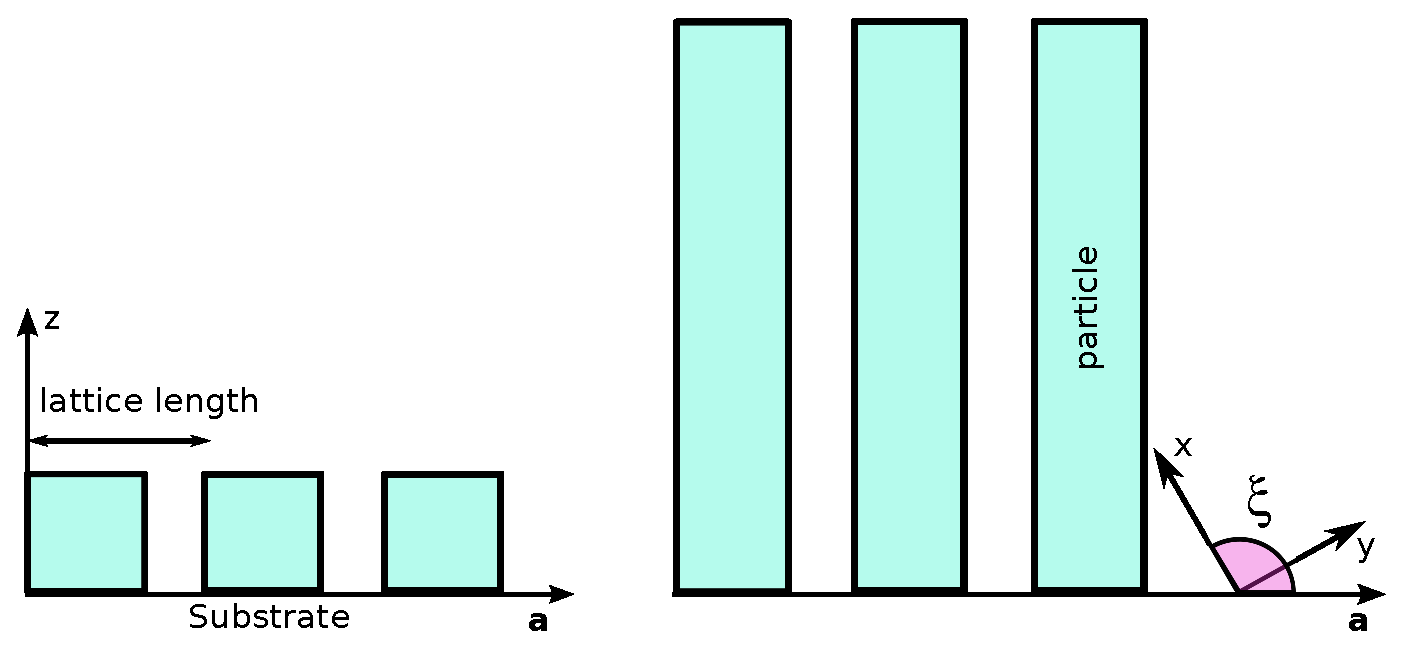
\includegraphics[width=0.75\textwidth]{Figures/1DGrating}
\end{center}
\caption{Schematic representation of a 1D lattice (side and top views). Such a lattice is characterized by a lattice length and the angle $\xi$.}
\label{fig:1dgrating}
\end{figure}

\ImportantPoint{Remark:}{By default the long axis of the particles in this 1D lattice is along the beam axis: $\xi=90^{\circ}$.}

\vspace{12pt}
A probability distribution function \Code{pdf} has to be chosen from the list in section~\ref{baftd} in order to apply some modifications to the scattering peaks. This function is implemented using \Code{setProbabilityDistribution(pdf)}. 

\paragraph{Example:} Script~\ref{lst:1dlattinterf} details how to build in  \BornAgain a sample using\\ \Code{InterferenceFunction1DLattice} as the interference function. As mentioned previously, this interference function can only be used with infinitely wide or long particles.\\ Here the sample is made of infinitely long boxes deposited on a substrate (these particles are characterized by their widths and heights). They are also rotated by $90^{\circ}$  in the sample surface in order to have their long axis perpendicular to the input beam, which is along the $x$-axis.\\
 The lattice parameters (the lattice lengths and angle between the lattice main axis and the $x$-axis) are specified using \Code{Lattice1DIFParameters()}. They are then used as input parameters of the interference function.

\newpage
\begin{lstlisting}[language=python, style=eclipseboxed,numbers=none,nolol,caption={\Code{Python} script to generate a sample made of infinitely long boxes deposited on a substrate layer with the 1DLatticeInterference function. The part specific to the interferences is marked in red italic font.},label={lst:1dlattinterf}]
def get_sample():
    """
    Build and return the sample with 1DLatticeInterference function
    """
    # defining materials
    m_air = HomogeneousMaterial("Air", 0.0, 0.0)
    m_substrate = HomogeneousMaterial("Substrate", 6e-6, 2e-8)
    m_particle = HomogeneousMaterial("Particle", 6e-4, 2e-8)

    # collection of particles
    ff = FormFactorInfLongBox(10.*nanometer, 15.0*nanometer)
    box = Particle(m_particle, ff)
    particle_layout = ParticleLayout()
    transform = Transform3D.createRotateZ(90.0*degree)
    particle_layout.addParticle(box, transform)

    # lattice parameters
    |lattice_params = Lattice1DIFParameters()|
    |lattice_params.m_length = 30.0*nanometer|
    |lattice_params.m_xi = 0.0*degree|

    # interference function
    |interference = InterferenceFunction1DLattice(lattice_params)|
    |pdf = FTDistribution1DCauchy(200./2./M_PI*nanometer)|
    |interference.setProbabilityDistribution(pdf)|
    |particle_decoration.addInterferenceFunction(interference)|

    # air layer with particles and substrate form multi layer
    air_layer = Layer(m_air)
    air_layer.setDecoration(particle_decoration)
    substrate_layer = Layer(m_substrate, 0)

    multi_layer = MultiLayer()
    multi_layer.addLayer(air_layer)
    multi_layer.addLayer(substrate_layer)
    return multi_layer
\end{lstlisting} 

\newpage
%%%%%%%%%%%%%%%%%%%%%%%%%%%%%%%%%%%%%%%%%%
\subsubsection{\ding{253} \Code{InterferenceFunction1DParaCrystal(peak\_distance, width, corr\_length)}}  
\begin{itemize}
\item[where] \Code{peak\_distance} is the average distance to the first neighbor peak, 
\item[]\Code{width} is the width parameter of the probability distribution,
\item[] \Code{corr\_length} is the correlation length (equal to 0 by default).
\end{itemize}

For this particular interference function, the implemented probability distribution function is Gaussian:

\begin{equation*}
p(x)=\frac{1}{\omega \sqrt{2\pi}} \exp\left(-\dfrac{(x-D)^2}{\omega^2}\right),\qquad P(q_{\parallel})=\exp\left(-\frac{q_{\parallel}^2 \omega^2}{2}\right)\exp(iq_{\parallel}D)
\end{equation*}
where $\omega\equiv$\Code{width}, $D\equiv$ \Code{peak\_distance}, and $q_{\parallel}=\sqrt{\Re^2(q_x) + \Re^2(q_y)}$ (see fig.~\ref{fig:1dpara}).

\begin{figure}[h]
\begin{center}
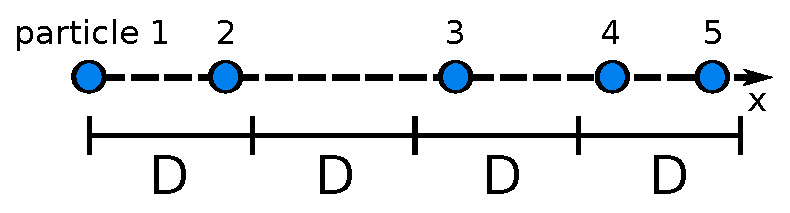
\includegraphics[width=0.5\textwidth]{Figures/1Dparacrystal}
\end{center}
\caption{Schematic representation of a 1D paracrystal in real space (side view). $D$ is the average spacing between the particles.}
\label{fig:1dpara}
\end{figure}

Using the procedure described in Section~\ref{sec:partlayout}, the interference function of a one-dimensional paracrystal is given by

\begin{align*}
S(q_{\parallel}) &=\Re \left(\frac{1+\Phi(q_{\parallel}) }{1 - \Phi(q_{\parallel})} \right), \\
\mathrm{where}\quad \Phi(q_{\parallel}) &= \left\{
\begin{array}{c l}     
    P(q_{\parallel}) & \mathrm{if\ \Code{corr\_length}}=0\\
    P(q_{\parallel})\exp\left(-\frac{D}{\mathrm{\Code{corr\_length}}}\right) & \mathrm{otherwise}
\end{array}\right.&
\end{align*}
Figure~\ref{fig:1dparas_q} shows the evolution of S(q) for different values of $\omega /D$. 
%$\kappa$  is the size-distance coupling constant (equal to 0 by default) for Size Spacing Correlation Approximation

\begin{figure}[h]
\begin{center}
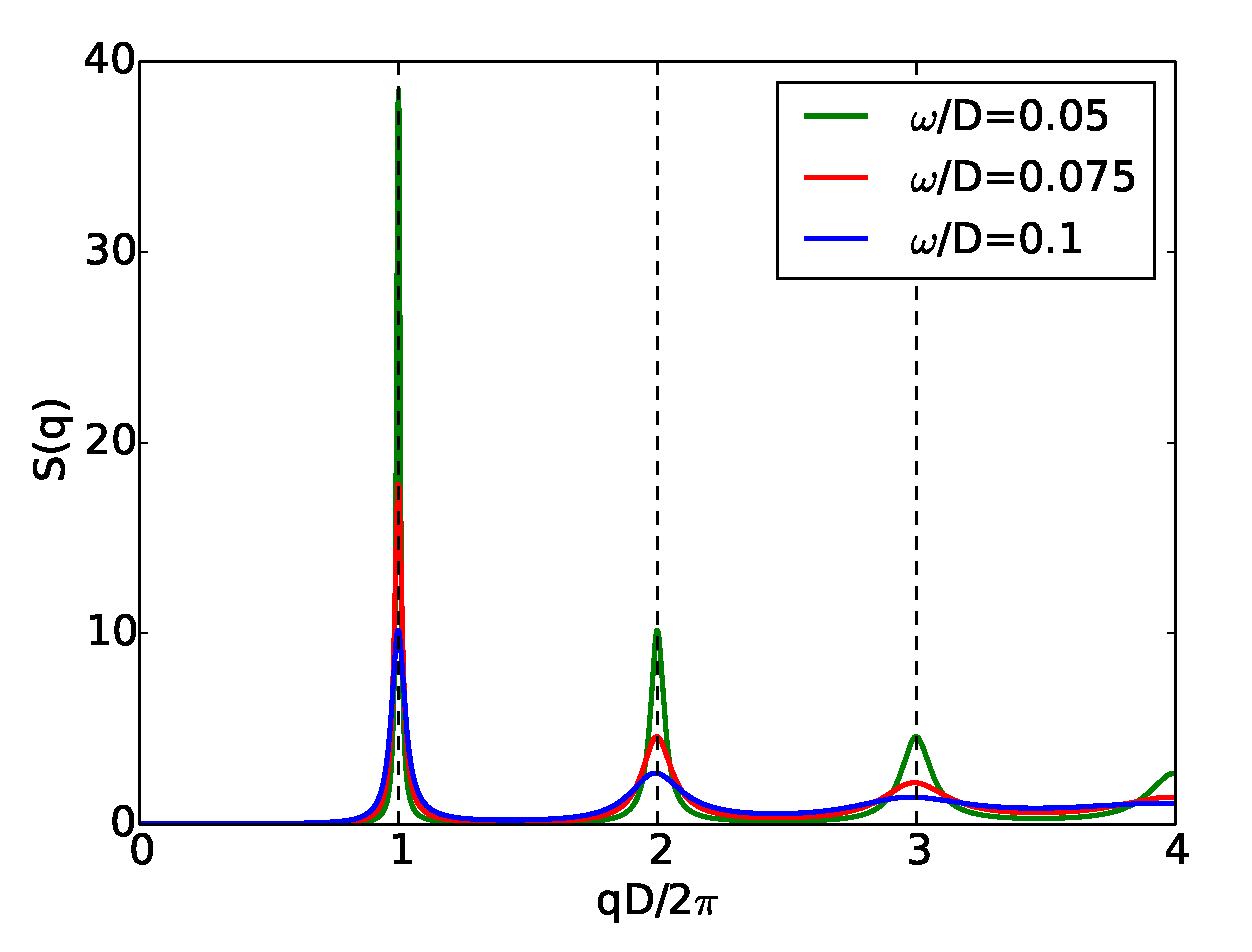
\includegraphics[width=0.65\textwidth]{Figures/S_q_1Dparacrystal}
\end{center}
\caption{Interference function of a 1D Gaussian paracrystal plotted for different values of $\omega /D$. The peaks broaden with a decreasing amplitude as $\omega/D$ increases. This shows the transition between an ordered and a disordered states. }
\label{fig:1dparas_q}
\end{figure}


\MakeRemark{Remark}{
In \BornAgain\, the one-dimensional disorder linked with this interference function is radial.
}

\paragraph{Example}
To illustrate the 1D paracrystal interference function, we use the same sample as in the case without interference: half-spheres deposited on a substrate.

\begin{lstlisting}[language=python, style=eclipseboxed,numbers=none,nolol,caption={\Code{Python} script to define the 1D paracrystal interference function between half-spheres, where \Code{trsphere} is of type \Code{Particle}.},label={lst:1dpara}]
    particle_layout = ParticleLayout()
    particle_layout.addParticle(trsphere, 0.0, 1.0)
    interference = InterferenceFunction1DParaCrystal(25.0*nanometer, 7*nanometer, 1e3*nanometer)
    particle_layout.addInterferenceFunction(interference)
\end{lstlisting}



\begin{figure}[h]
\begin{center}
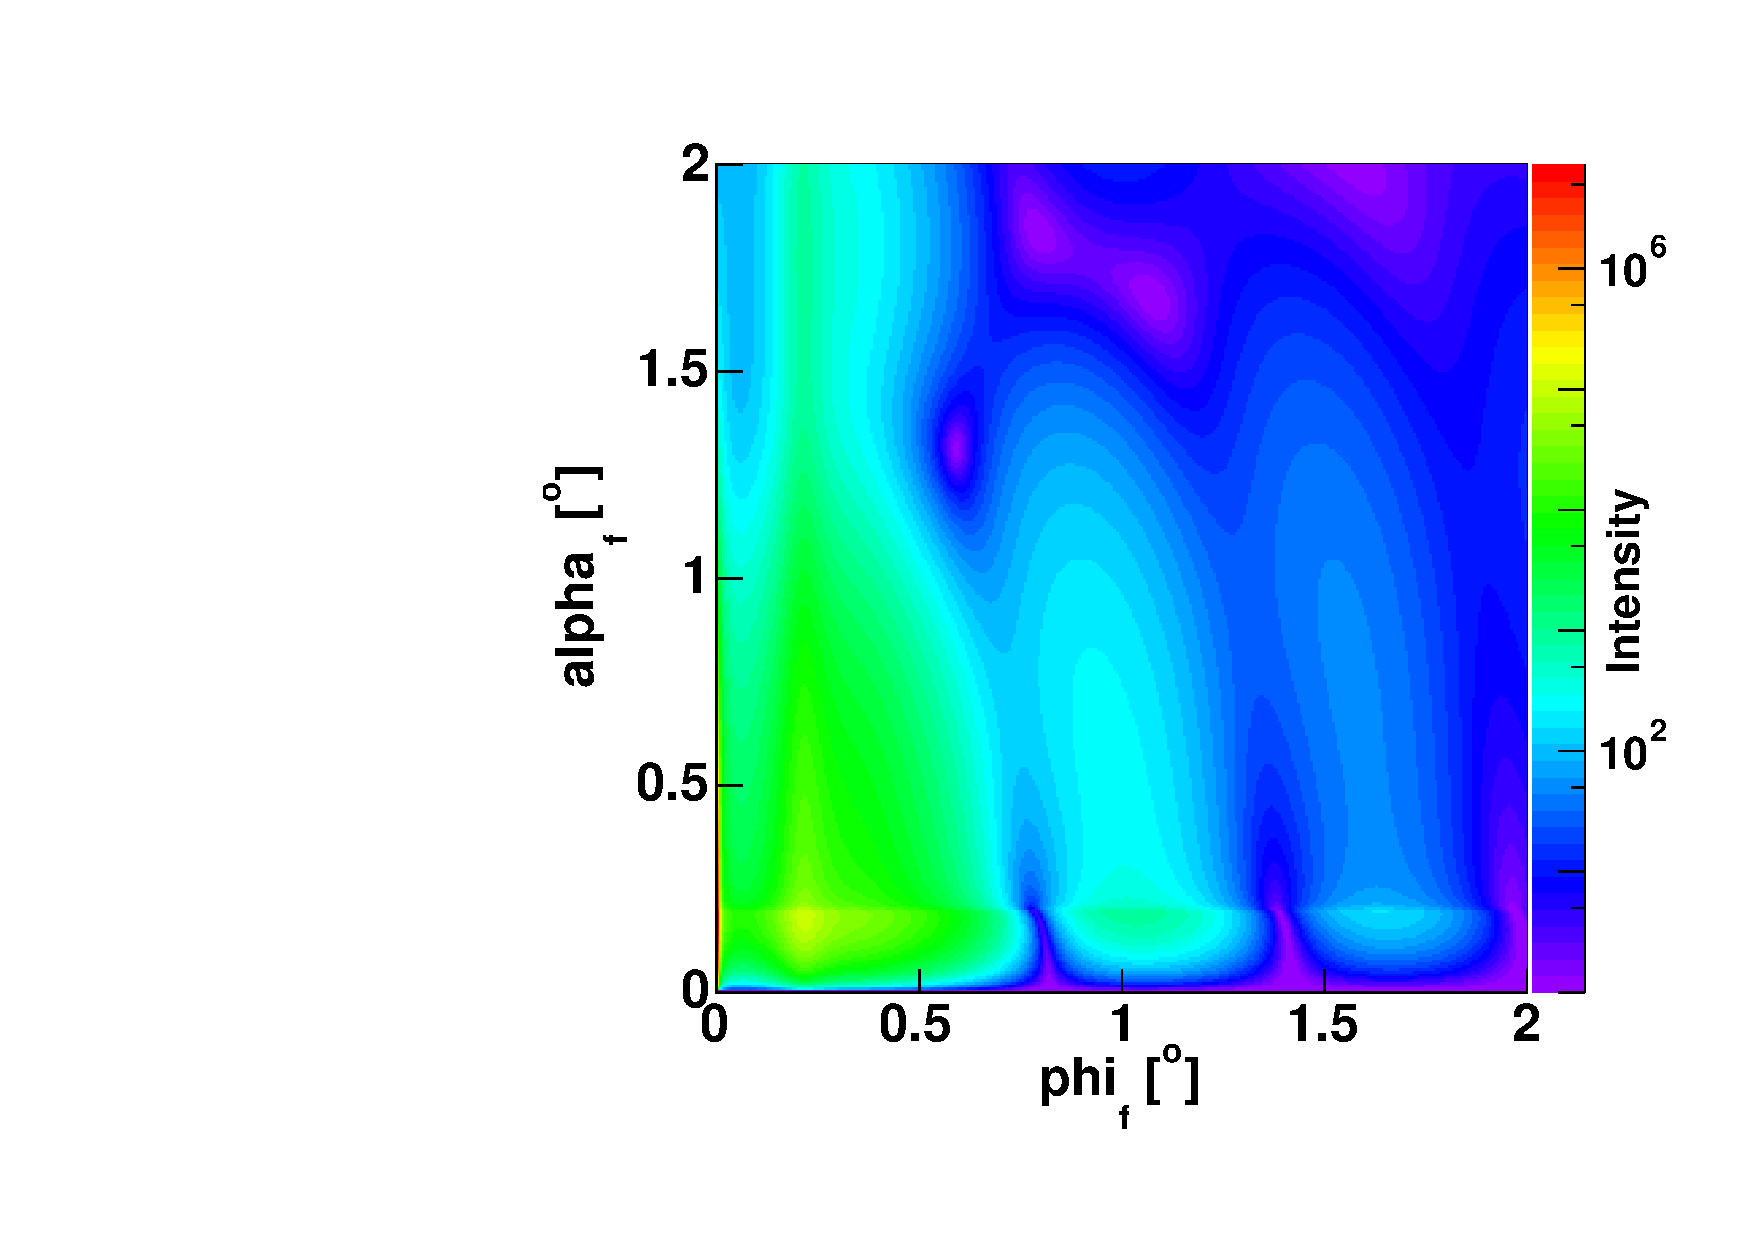
\includegraphics[width=0.5\textwidth]{Figures/HSphere_1DDL}
\end{center}
\caption{Output intensity scattered from a sample made of half-spheres with 1Dparacrystal interference between them. This figure has been generated using Script~\ref{lst:1dpara} for the interference function. The full script UMInterferences1DParaCrystal.py can be found in /Examples/python/UserManual.}
\label{fig:1ddl}
\end{figure}

\FloatBarrier

\newpage%{\cleardoublepage}
%%%%%%%%%%%%%%%%%%%%%%%%%%%%%%%%%%%%%%
\subsubsection{\ding{253}  \Code{InterferenceFunction2DLattice(lattice\_parameters)}} 
where \Code{lattice\_parameters} corresponds to ($L_1$, $L_2$, $\alpha$, $\xi$)  (see illustration in figure~\ref{fig:2dlattice}) with 
\begin{itemize}
\item[]$L_1$, $L_2$ the lengths of the lattice cell, 
\item[]$\alpha$ the angle between the lattice basis vectors $\mathbf{a}, \mathbf{b}$ in direct space,
\item[] $\xi$ is the angle defining the lattice orientation (set to $0$ by default); it is taken as the angle between the $\mathbf{a}$ vector of the lattice basis and the $\mathbf{x}$ axis of the "GISAS experiment" referential (as shown in figure~\ref{fig:multil3d}).
\end{itemize}

\begin{figure}[h]
\begin{center}
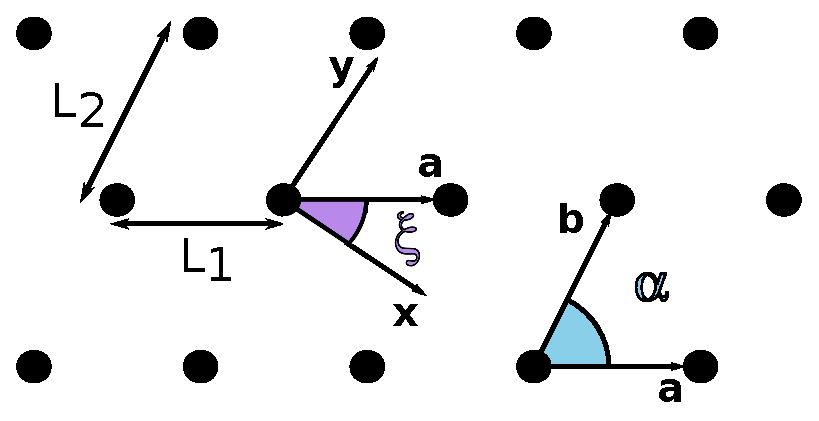
\includegraphics[width=0.5\textwidth]{Figures/2Dlattice.eps}
\end{center}
\caption{Schematic representation of a 2D lattice (top view). Such a lattice is characterized by lattice lengths $L_1$, $L_2$ and angles $\alpha$ and $\xi$.}
\label{fig:2dlattice}
\end{figure}

Like for the one-dimensional case, a probability distribution function \Code{pdf} has to be defined. One can choose between those listed in Section~\ref{baftd} and implements it using \Code{setProbabilityDistribution(pdf)}.

\paragraph{Example} The sample used to run the simulation is made of half-spheres deposited on a substrate. The interference function is "2Dlattice" and the particles are located at the nodes of a square lattice with $L_1=L_2=20$~nm, $\mathbf{a}\equiv \mathbf{b}$ and the probability distribution function is Gaussian. We also use the Local Monodisperse Approximation. 

\begin{lstlisting}[language=python, style=eclipseboxed,numbers=none,nolol,caption={\Code{Python} script to define a 2DLattice interference function between hemi-spherical particles as well as the Local Monodisperse Approximation in \Code{getSimulation()}.  The part specific to the interferences is marked in red italic font.},label={lst:2dlatticeinterf}]
    # lattice parameters
    |lattice_params = Lattice2DIFParameters()|
    |lattice_params.m_length_1 = 20.0*nanometer|
    |lattice_params.m_length_2 = 20.0*nanometer|
    |lattice_params.m_angle = 90.0*degree|
    |lattice_params.m_xi = 0.0*degree|

    #collection of particles
    sphere_ff = FormFactorTruncatedSphere(5*nanometer, 5*nanometer)
    sphere = Particle(m_particle, sphere_ff)
    |interference = InterferenceFunction2DLattice(lattice_params)|
    |pdf = FTDistribution2DGauss(200.0*nanometer/2.0/M_PI, 75.0*nanometer/2.0/M_PI)|
    |interference.setProbabilityDistribution(pdf)|
    particle_layout = ParticleLayout()
    particle_layout.addParticle(sphere, 0.0, 1.0)
    |particle_layout.addInterferenceFunction(interference)|
\end{lstlisting}
 
\begin{lstlisting}[language=python, style=eclipseboxed,numbers=none,nolol]
def get_simulation():
    """
    Create and return GISAXS simulation with beam and detector
    """
    simulation = Simulation()
    simulation.setDetectorParameters(100, 0.0*degree, 2.0*degree, 100, 0.0*degree, 2.0*degree)
    simulation.setBeamParameters(1.0*angstrom, 0.2*degree, 0.0*degree)
    |sim_params= SimulationParameters()|
    |sim_params.me_if_approx = SimulationParameters.LMA|
    |simulation.setSimulationParameters(sim_params)|
    return simulation
\end{lstlisting}


\begin{figure}[h]
\begin{center}
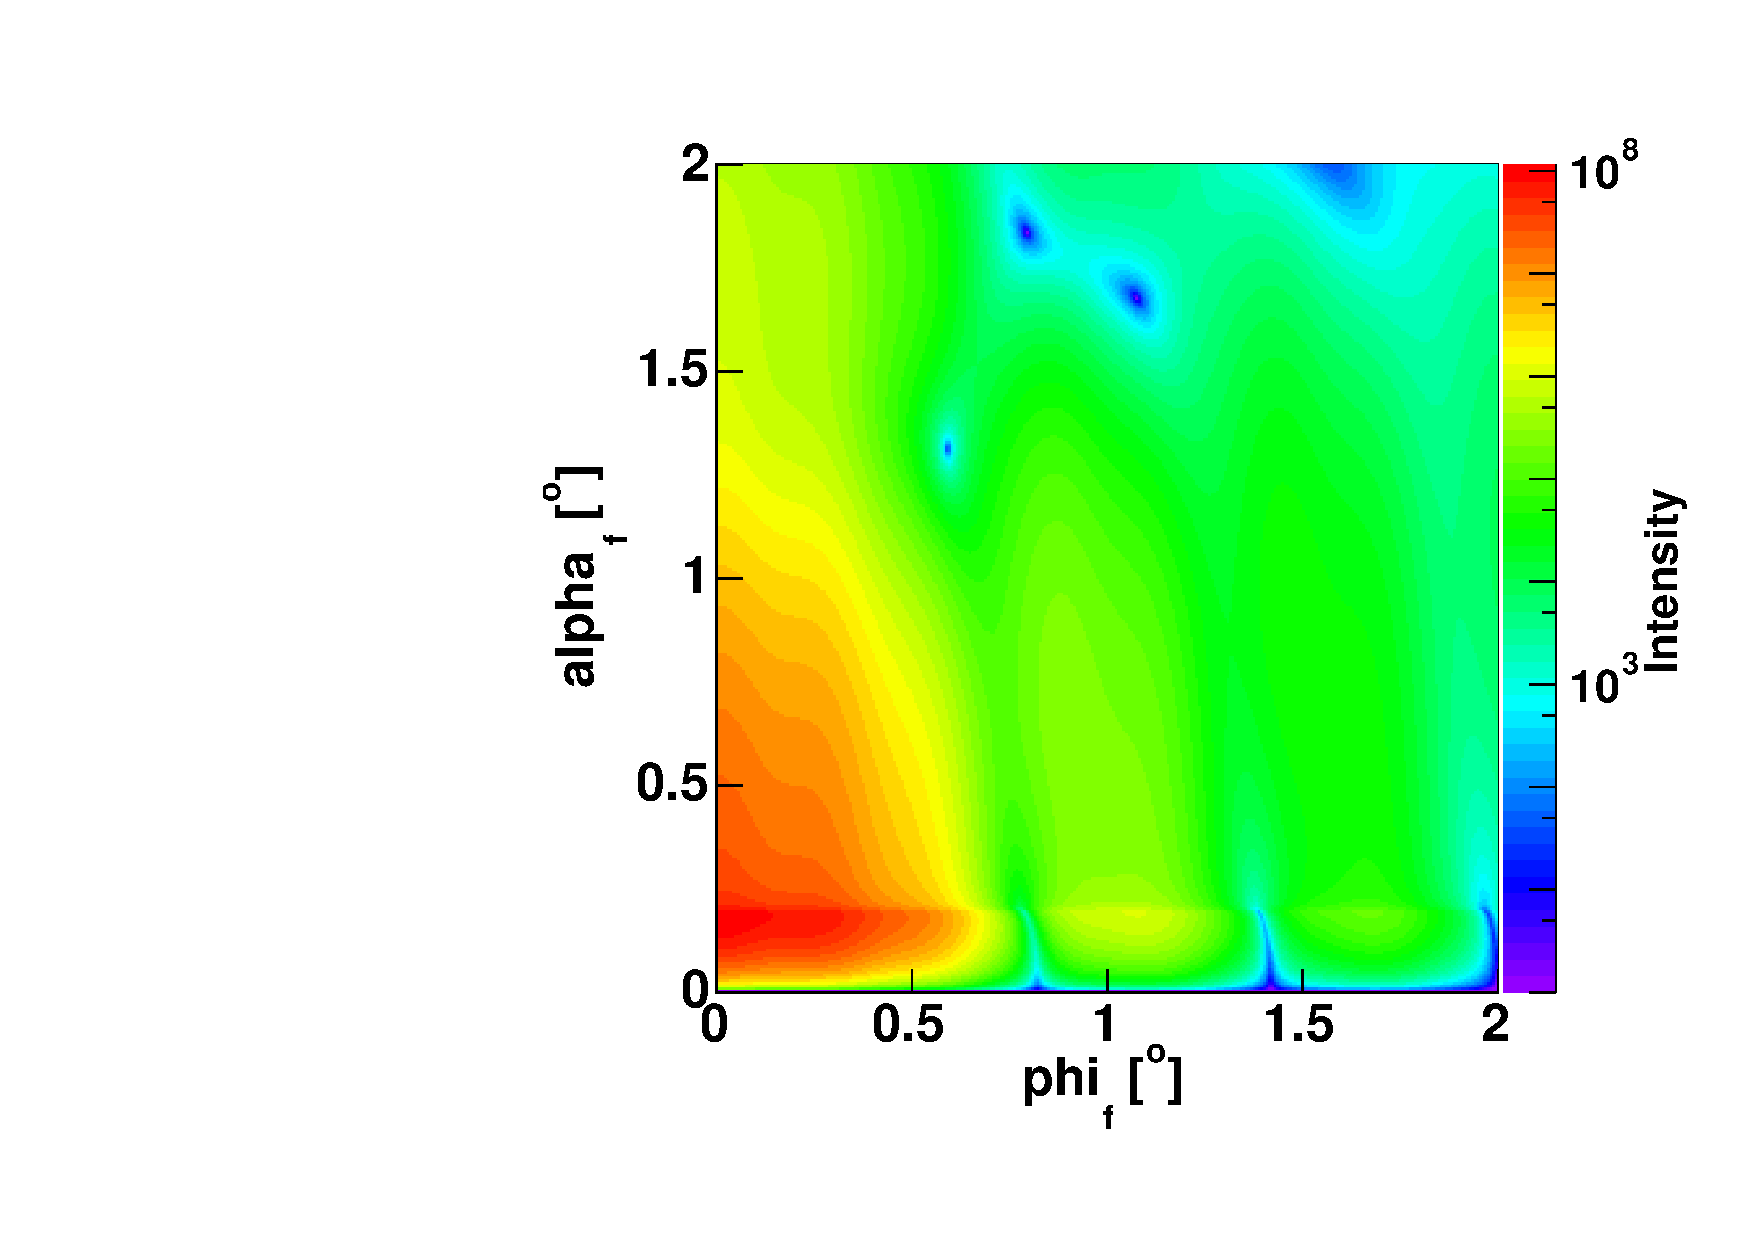
\includegraphics[width=0.5\textwidth]{Figures/HSphere_2Dlattice}
\end{center}
\caption{Output intensity scattered from a sample made of half-spheres with 2DLattice interference function. \Python\ script available in {/Examples/python/UserManual/UMInterferences2DLattice.py}.}
\label{fig:2dlatticeintensity}
\end{figure}

\FloatBarrier

\newpage%{\cleardoublepage}
%%%%%%%%%%%%%%%%%%%%%%%%%%%%%%%%%%%%%%%
\subsubsection{\ding{253} \Code{InterferenceFunction2DParaCrystal(L\_1, L\_2, lattice\_angle, $\xi$, damping\_length)}} 
\begin{itemize}
\item[where] $L_1$, $L_2$ are the lengths of the lattice cell,
\item[] lattice\_angle the angle between the lattice basis vectors $\mathbf{a}, \mathbf{b}$ in direct space,
\item[] $\xi$ is the angle defining the lattice orientation (set to $0$ by default).
\item[] \Code{damping\_length} is a "damping" length. It is used to introduce finite size effects by applying a multiplicative coefficient equal to  $\exp$(\Code{peak\_distance/damping\_length}) to the Fourier transform of the probability densities. \Code{damping\_length} is equal to 0 by default and, in this case, no correction is applied.
\end{itemize}
Two predefined interference functions can also be used:
\begin{itemize}
\item  \Code{createSquare(peak\_distance, damping\_length, domain\_size\_1, domain\_size\_2)}\\
where the angle between the base vectors of the lattice is set to $\pi/2$,
it creates a squared lattice,
\item \Code{createHexagonal(peak\_distance, damping\_length, domain\_size\_1, domain\_size\_2)}\\
where the angle between the base vectors of the lattice is set to $2\pi/3$ ,
\end{itemize}
where
\Code{domain\_size1, 2} are the dimensions of coherent domains of the paracrystal along the main axes,\\ \Code{peak\_distance} is the same in both directions and $\mathbf{a}\equiv \mathbf{x}$.\\

Probability distribution functions have to be defined. As the two-dimensional paracrystal is defined from two independent 1D paracrystals, we need two of these functions, using\\ \Code{setProbabilityDistributions(pdf\_1, pdf\_2)}, with \Code{pdf\_{1,2}} are related to each main axis of the paracrystal (see figure~\ref{fig:2dparaschematic}).


\begin{figure}[h]
\begin{center}
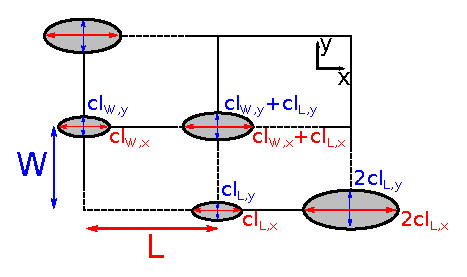
\includegraphics[width=0.75\textwidth]{Figures/drawing2Dparacrystal.eps}
\end{center}
\caption{Shematics of the ideal 2D paracrystal. The grey-shaded areas mark the regions where the probability to find a node is larger that the width at half-maximum of the distribution. $L$ and  $W$ are the mean inter-node distances along the two crystallographic axes. cl$_{(L,W),(x,y)}$ are the widths of the distribution of distance. The disorder is propagated as we add more nodes. Such a structure would be generated using \Code{InterferenceFunction2DParacrystal(L,W,90.*degrees,0,damp\_length)}, with \Code{pdf$_1$ = FTDistribution2DGauss(cl$_{L,x}$,cl$_{L,y}$)} and  \Code{pdf$_2$ = FTDistribution2DGauss(cl$_{W,x}$,cl$_{W,y}$)}.}
\label{fig:2dparaschematic}
\end{figure}


\paragraph{Example} The particles deposited on a substrate are half-spheres. The scattered beams interference via the 2DParacrystal distribution function. The paracrystal is based on a 2D hexagonal lattice with a Gaussian probability distribution function in reciprocal space.  Script~\ref{lst:2dlatticeinterf} shows the implementation of the interference function and fig.~\ref{fig:2ddl} an example of output intensity using hemi-spherical particles The full script, UMInterferences2DParacrystal.py is available in /Examples/python/UserManual.

\begin{lstlisting}[language=python, style=eclipseboxed,numbers=none,nolol,caption={\Code{Python} script to define a "2DParacrystal" interference function between particles forming an hexagonal monolayer. },label={lst:2dlatticeinterf}]
    interference = InterferenceFunction2DParaCrystal.createHexagonal(30.0*nanometer,0.0, 40.0*micrometer, 40.0*micrometer)|
    pdf = FTDistribution2DCauchy(1.0*nanometer, 1.0*nanometer)
    interference.setProbabilityDistributions(pdf, pdf)
    particle_decoration.addInterferenceFunction(interference)
\end{lstlisting}

\begin{figure}[h]
\begin{center}
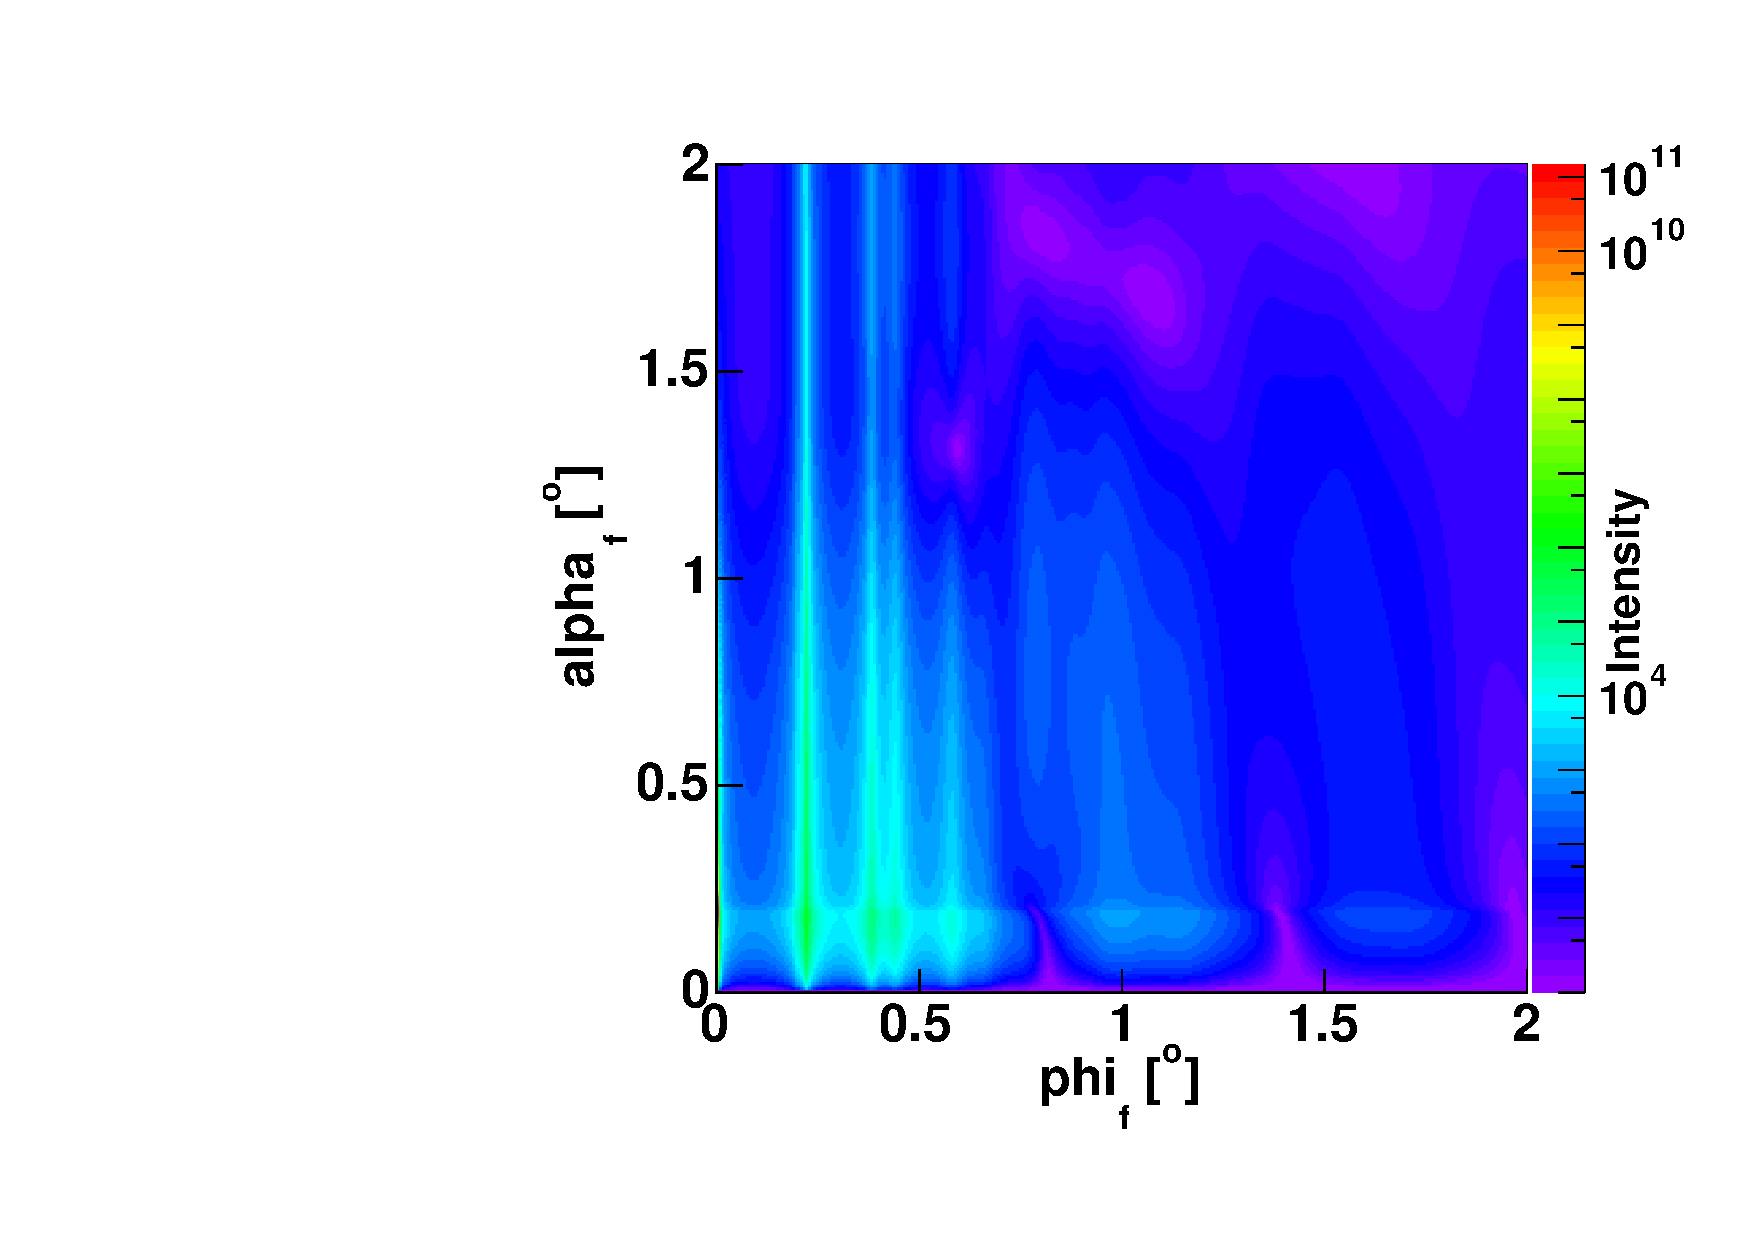
\includegraphics[width=0.5\textwidth]{Figures/HSphere_2DDL}
\end{center}
\caption{Output intensity scattered from a sample made of half-spheres with 2DParacrystal interference function.}
\label{fig:2ddl}
\end{figure}

\FloatBarrier

%%%%%%%%%%%%%%%%%%%%%%%%%%%%%%%%%%%%%%%%
\subsection{Summary}

\begin{landscape}
\begin{table}
\begin{tabular}{lll}
\hline
Function  & Parameters & Comments\\
\hline
\Code{InterferenceFunctionNone}  & None & disordered distribution \\
\hline
\Code{InterferenceFunction1DLattice} & \Code{lattice\_length} & use only with infinitely long/wide particles \\
  & $\xi=\widehat{(\mathbf{x},\mathbf{a})}$ & pdf=(Cauchy, Gauss or Voigt)  to be defined\\
\hline
 \Code{InterferenceFunction1DParaCrystal}  & peak\_distance of pdf & only Gaussian pdf implemented (no option)\\
   & width of pdf &\\
& corr\_length (optional) & \\
\hline
 \Code{InterferenceFunction2DLattice}  & L\_1, L\_2: lattice lengths & pdf=(Cauchy, Gauss or Voigt) to be defined\\
                        & lattice\_angle=$\widehat{(\mathbf{a},\mathbf{b})}$ & \\
                                                            & $\xi =\widehat{(\mathbf{x},\mathbf{a})}$ & \\                                                  
\hline
\Code{InterferenceFunction2DParaCrystal}  & L\_1, L\_2: lattice lengths & 2D pdf=(Cauchy, Gauss or Voigt) to be defined \\
                          & lattice\_angle=$\widehat{(\mathbf{a},\mathbf{b})}$ & (1 pdf per axis) \\
& $\xi=\widehat{(\mathbf{x},\mathbf{a})}$ & \\
& damping\_length (optional)  &  same for both axes\\
\hline
\hline
\end{tabular}
\caption{List of interference functions implemented in \BornAgain. pdf : probability distribution function, $\mathbf{a}, \mathbf{b}$ are the lattice base vector, and $\mathbf{x}$ is the axis vector perpendicular to the detector plane.}
\end{table}
\end{landscape}

%%%%%%%%%%%%%%%%%%%%%%%%%%%%%%%
\section{Particles - Form factors} \SecLabel{sect:ff}

\subsection{Born approximation}

In \BornAgain\ the form factor is defined using Born approximation as
\begin{equation}
F(\mathbf{q})=\int_V \exp (i\mathbf{q}.\mathbf{r}) d^3 \mathbf{r},
\label{ffformulaBA}
\end{equation}
where $V$ is the volume of the particle,
$\mathbf{q}=\mathbf{k}_i - \mathbf{k}_f$ is the scattering vector with
$\mathbf{k}_f$ and $\mathbf{k}_i$ the scattered and incident wave
vector, respectively.\\

The particle's shape is parametrized in a cartesian frame, with its
$z$-axis pointing upwards and its origin at the center of the bottom
of the particle: $\mathbf{r}=(x,y,z)$. 

All form factors have been implemented with complex scattering vectors
in order to take any material absorption into account.

Table~\ref{tab:formfactors} lists the shapes whose form
factors have been implemented in \BornAgain\ and a detailed description is given in Appendix \ref{appendixff}.

\newpage

\begin{table}[H] 
\caption{Table of form factors implemented in \BornAgain.} \label{tab:formfactors}
  \begin{tabulary} {\textwidth}{Lc Lc L c L} 
\hline 
Box,\phantom{-} \SecRef{Box} & & Prism3,  \SecRef{Prism3} & & Tetrahedron, \SecRef{Tetrahedron} & & Prism6,  \SecRef{Prism6}\\
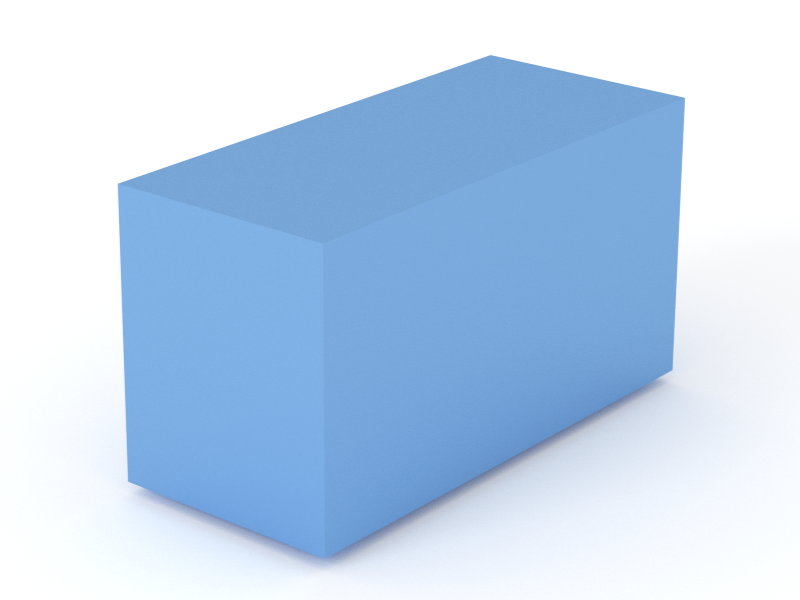
\includegraphics[width=1in]{Figures/Box3d} & & 
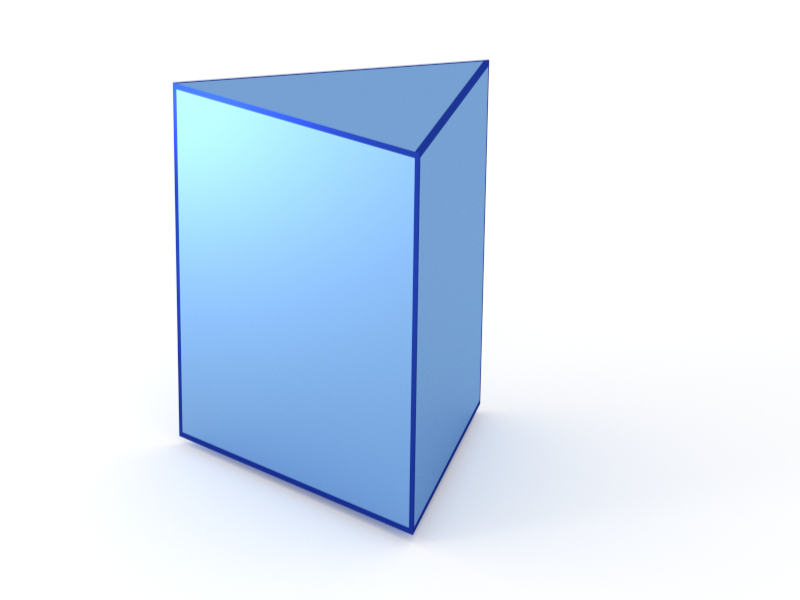
\includegraphics[width=1in]{Figures/Prism33d} & & 
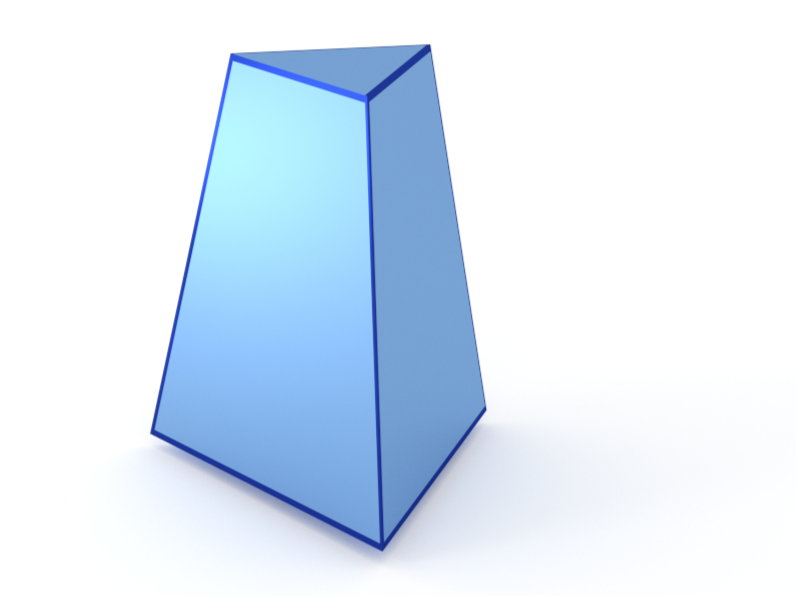
\includegraphics[width=1in]{Figures/Tetrahedron3d} & & 
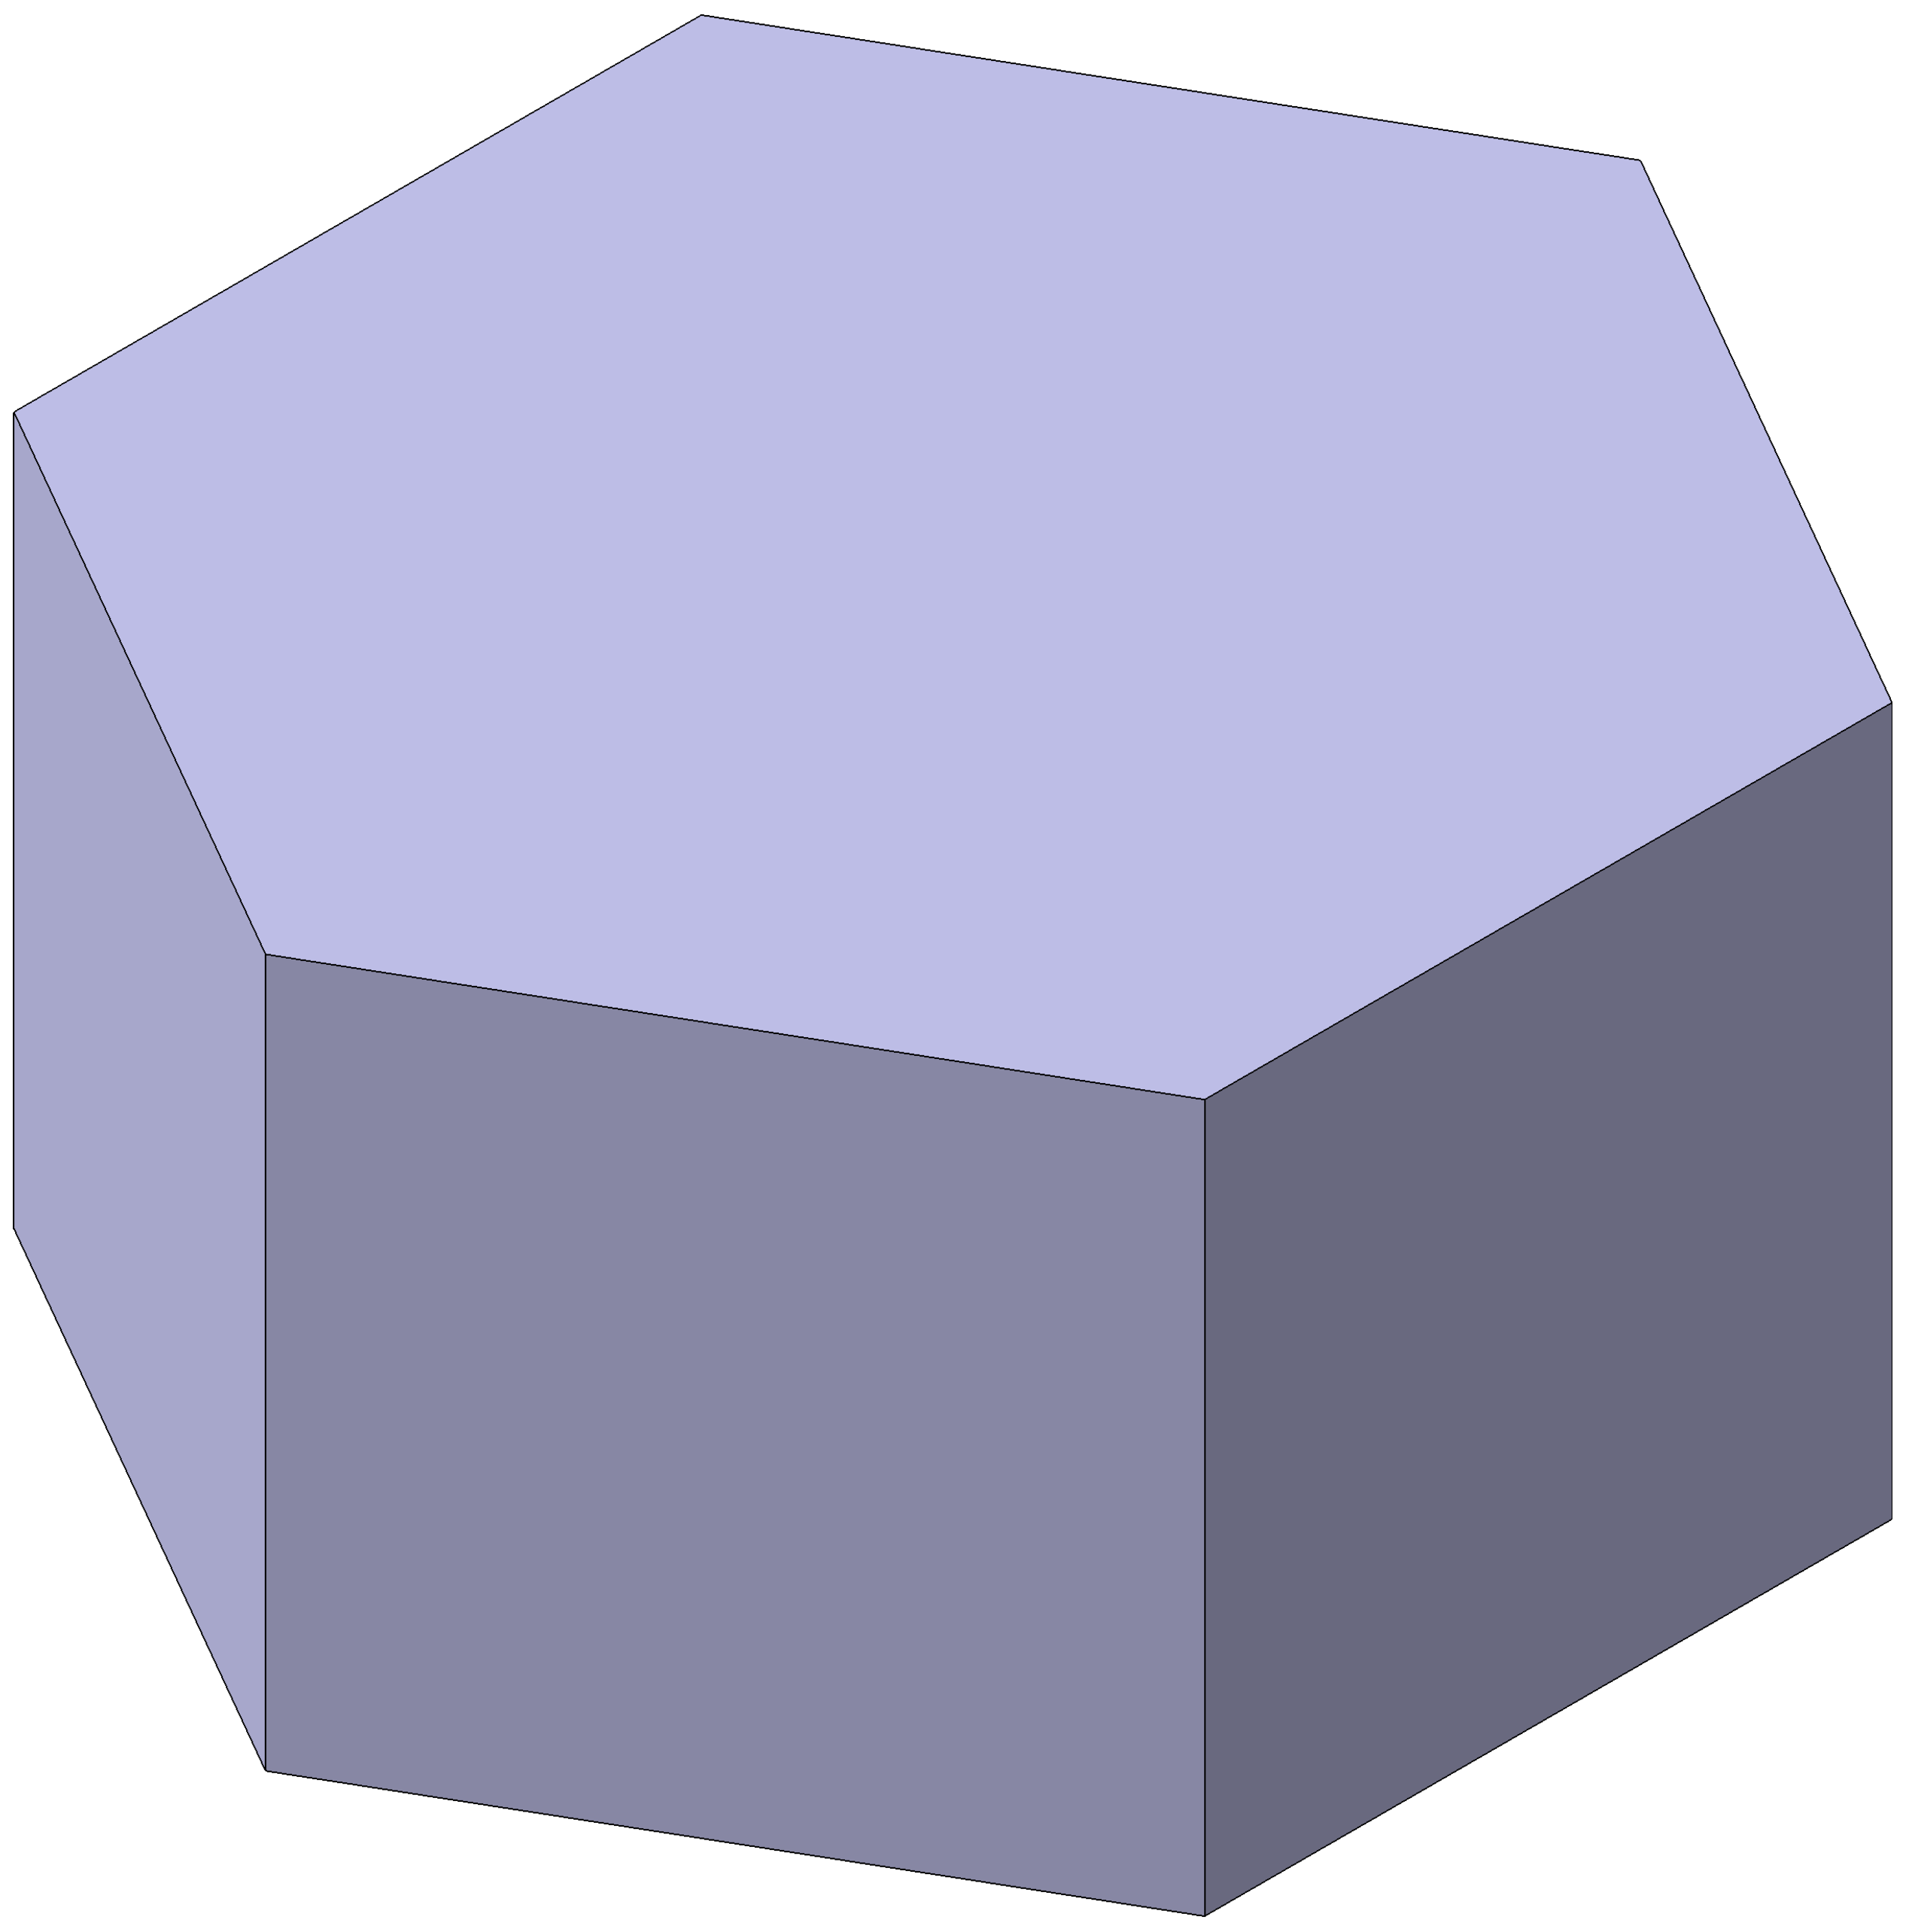
\includegraphics[width=1in]{Figures/Prism63d} 
\\
\hline 
Cone6,  \SecRef{Cone6} & &  Pyramid, \SecRef{Pyramid} & & Anisotropic pyramid,  \SecRef{AnisoPyramid} & &  {Cuboctahedron}, \SecRef{Cuboctahedron}\\
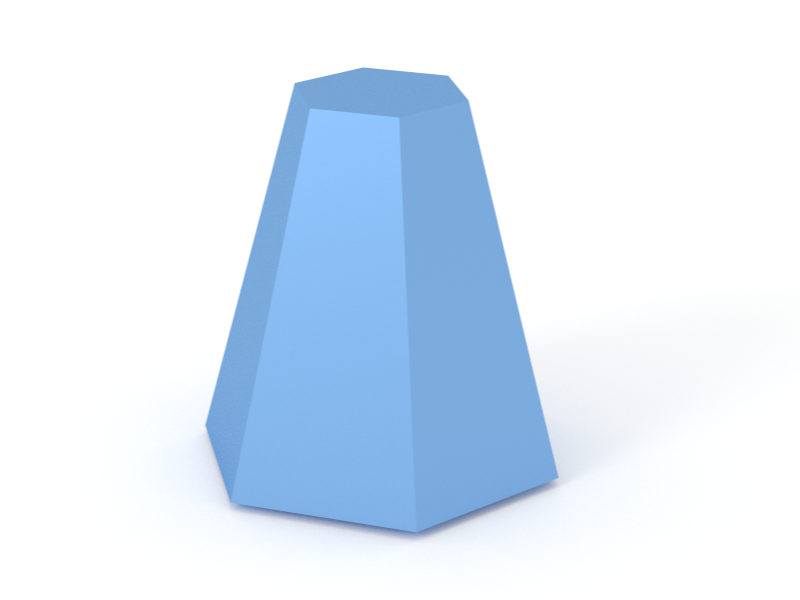
\includegraphics[width=1in]{Figures/Cone63d}  & & 
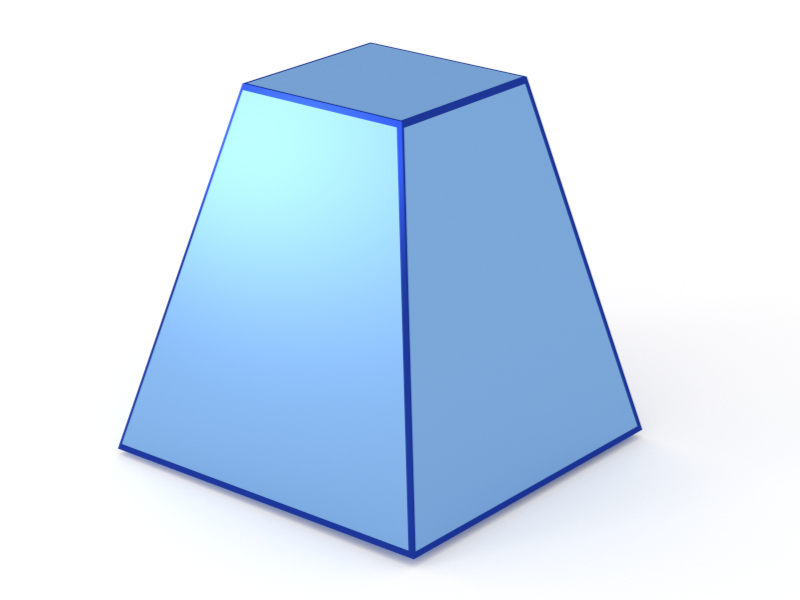
\includegraphics[width=1in]{Figures/Pyramid3d} & &
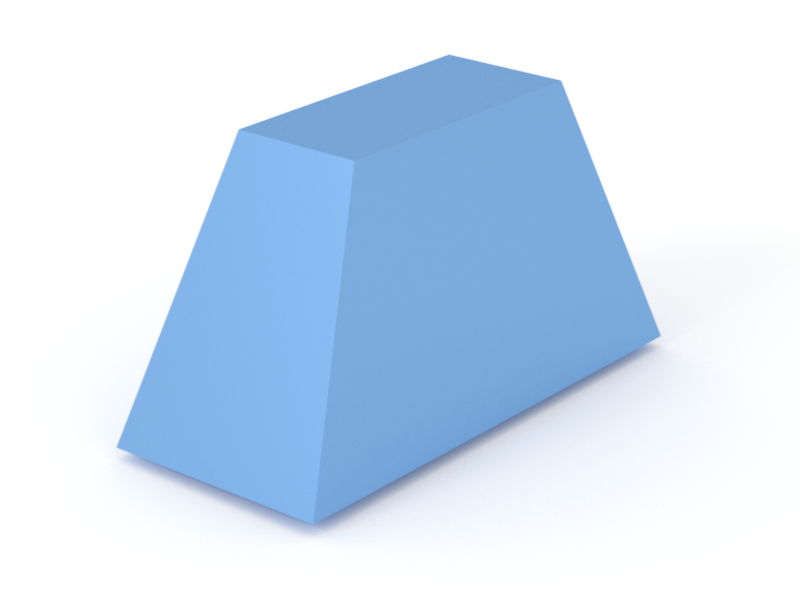
\includegraphics[width=1in]{Figures/AnistropicPyramid3d} & & 
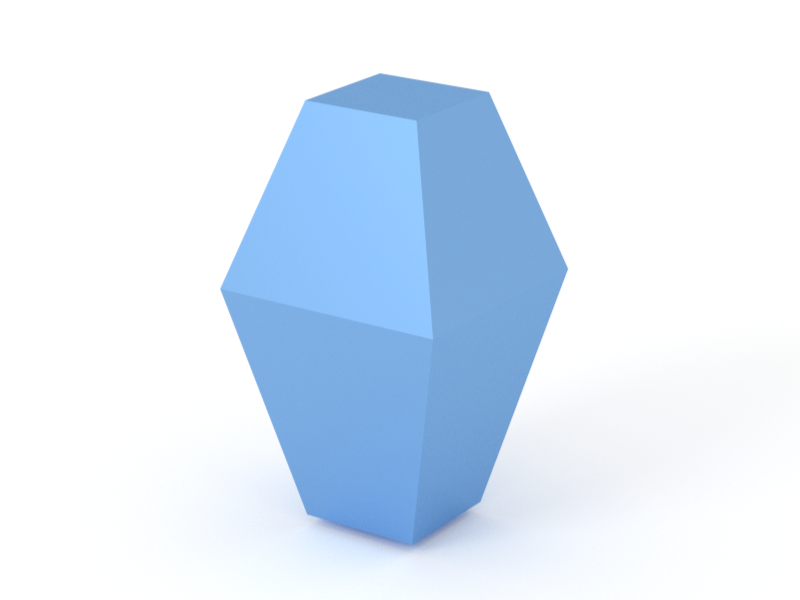
\includegraphics[width=1in]{Figures/Cuboctahedron3d}
\\
\hline
Cylinder, \SecRef{Cylinder}  & & Ellipsoidal cylinder, \SecRef{EllipsoidalCylinder} & &  Cone,\phantom{--} \SecRef{Cone} & & Full Sphere, \SecRef{FullSphere} \\
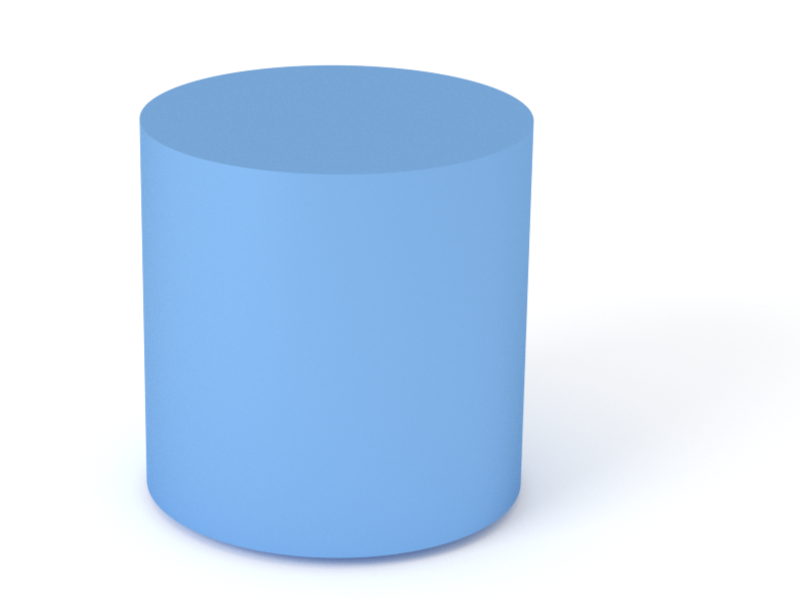
\includegraphics[width=1in]{Figures/Cylinder3d} & & 
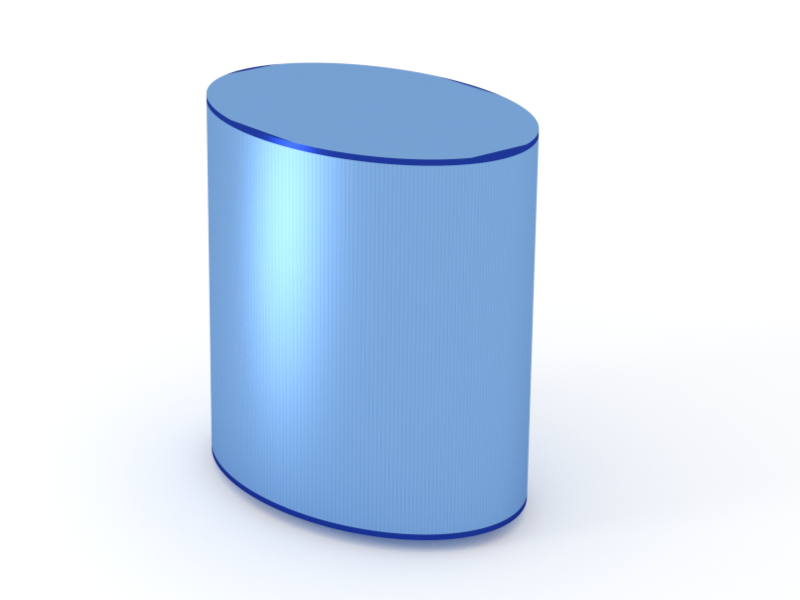
\includegraphics[width=1in]{Figures/EllipsoidalCylinder3d} & & 
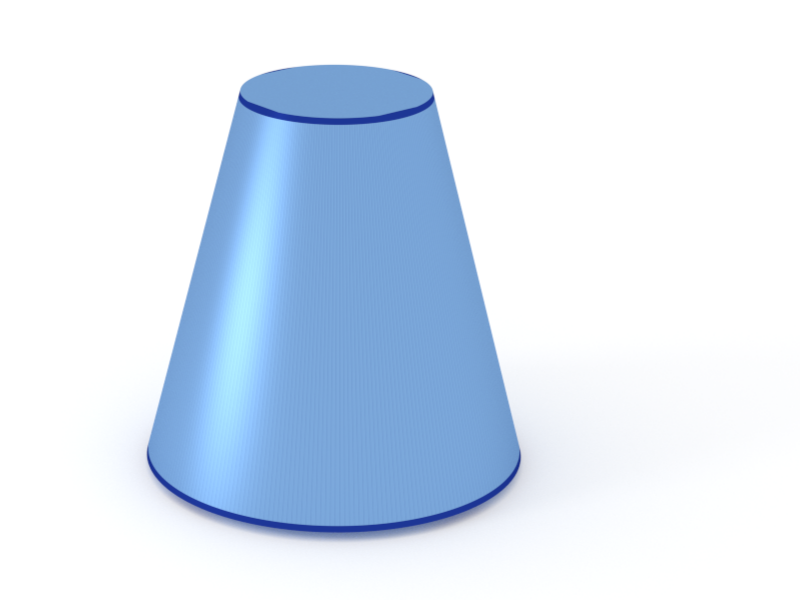
\includegraphics[width=1in]{Figures/Cone3d} & & 
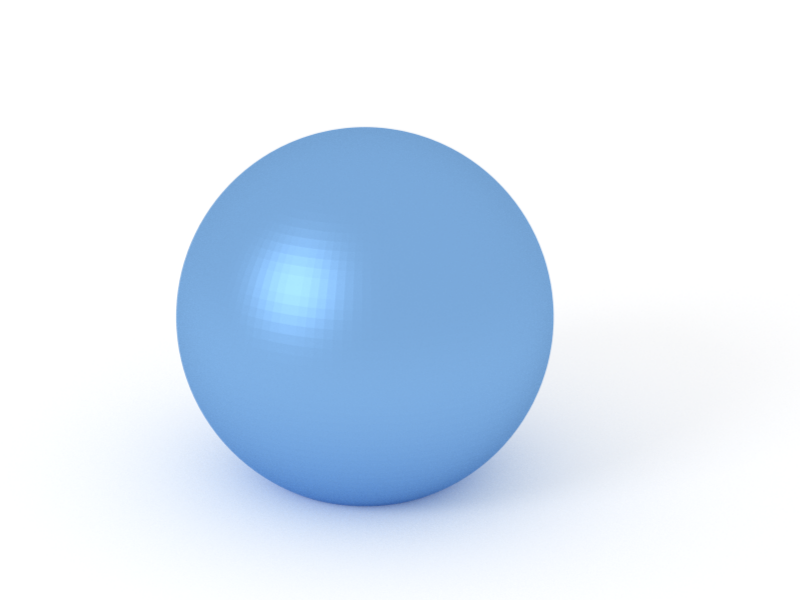
\includegraphics[width=1in]{Figures/FullSphere3d} \\
\hline
Truncated Sphere, \SecRef{Sphere}  & & Full Spheroid, \SecRef{FullSpheroid} & & Truncated Spheroid,  \SecRef{Spheroid} & & Hemi Ellipsoid, \SecRef{HemiEllipsoid}\\
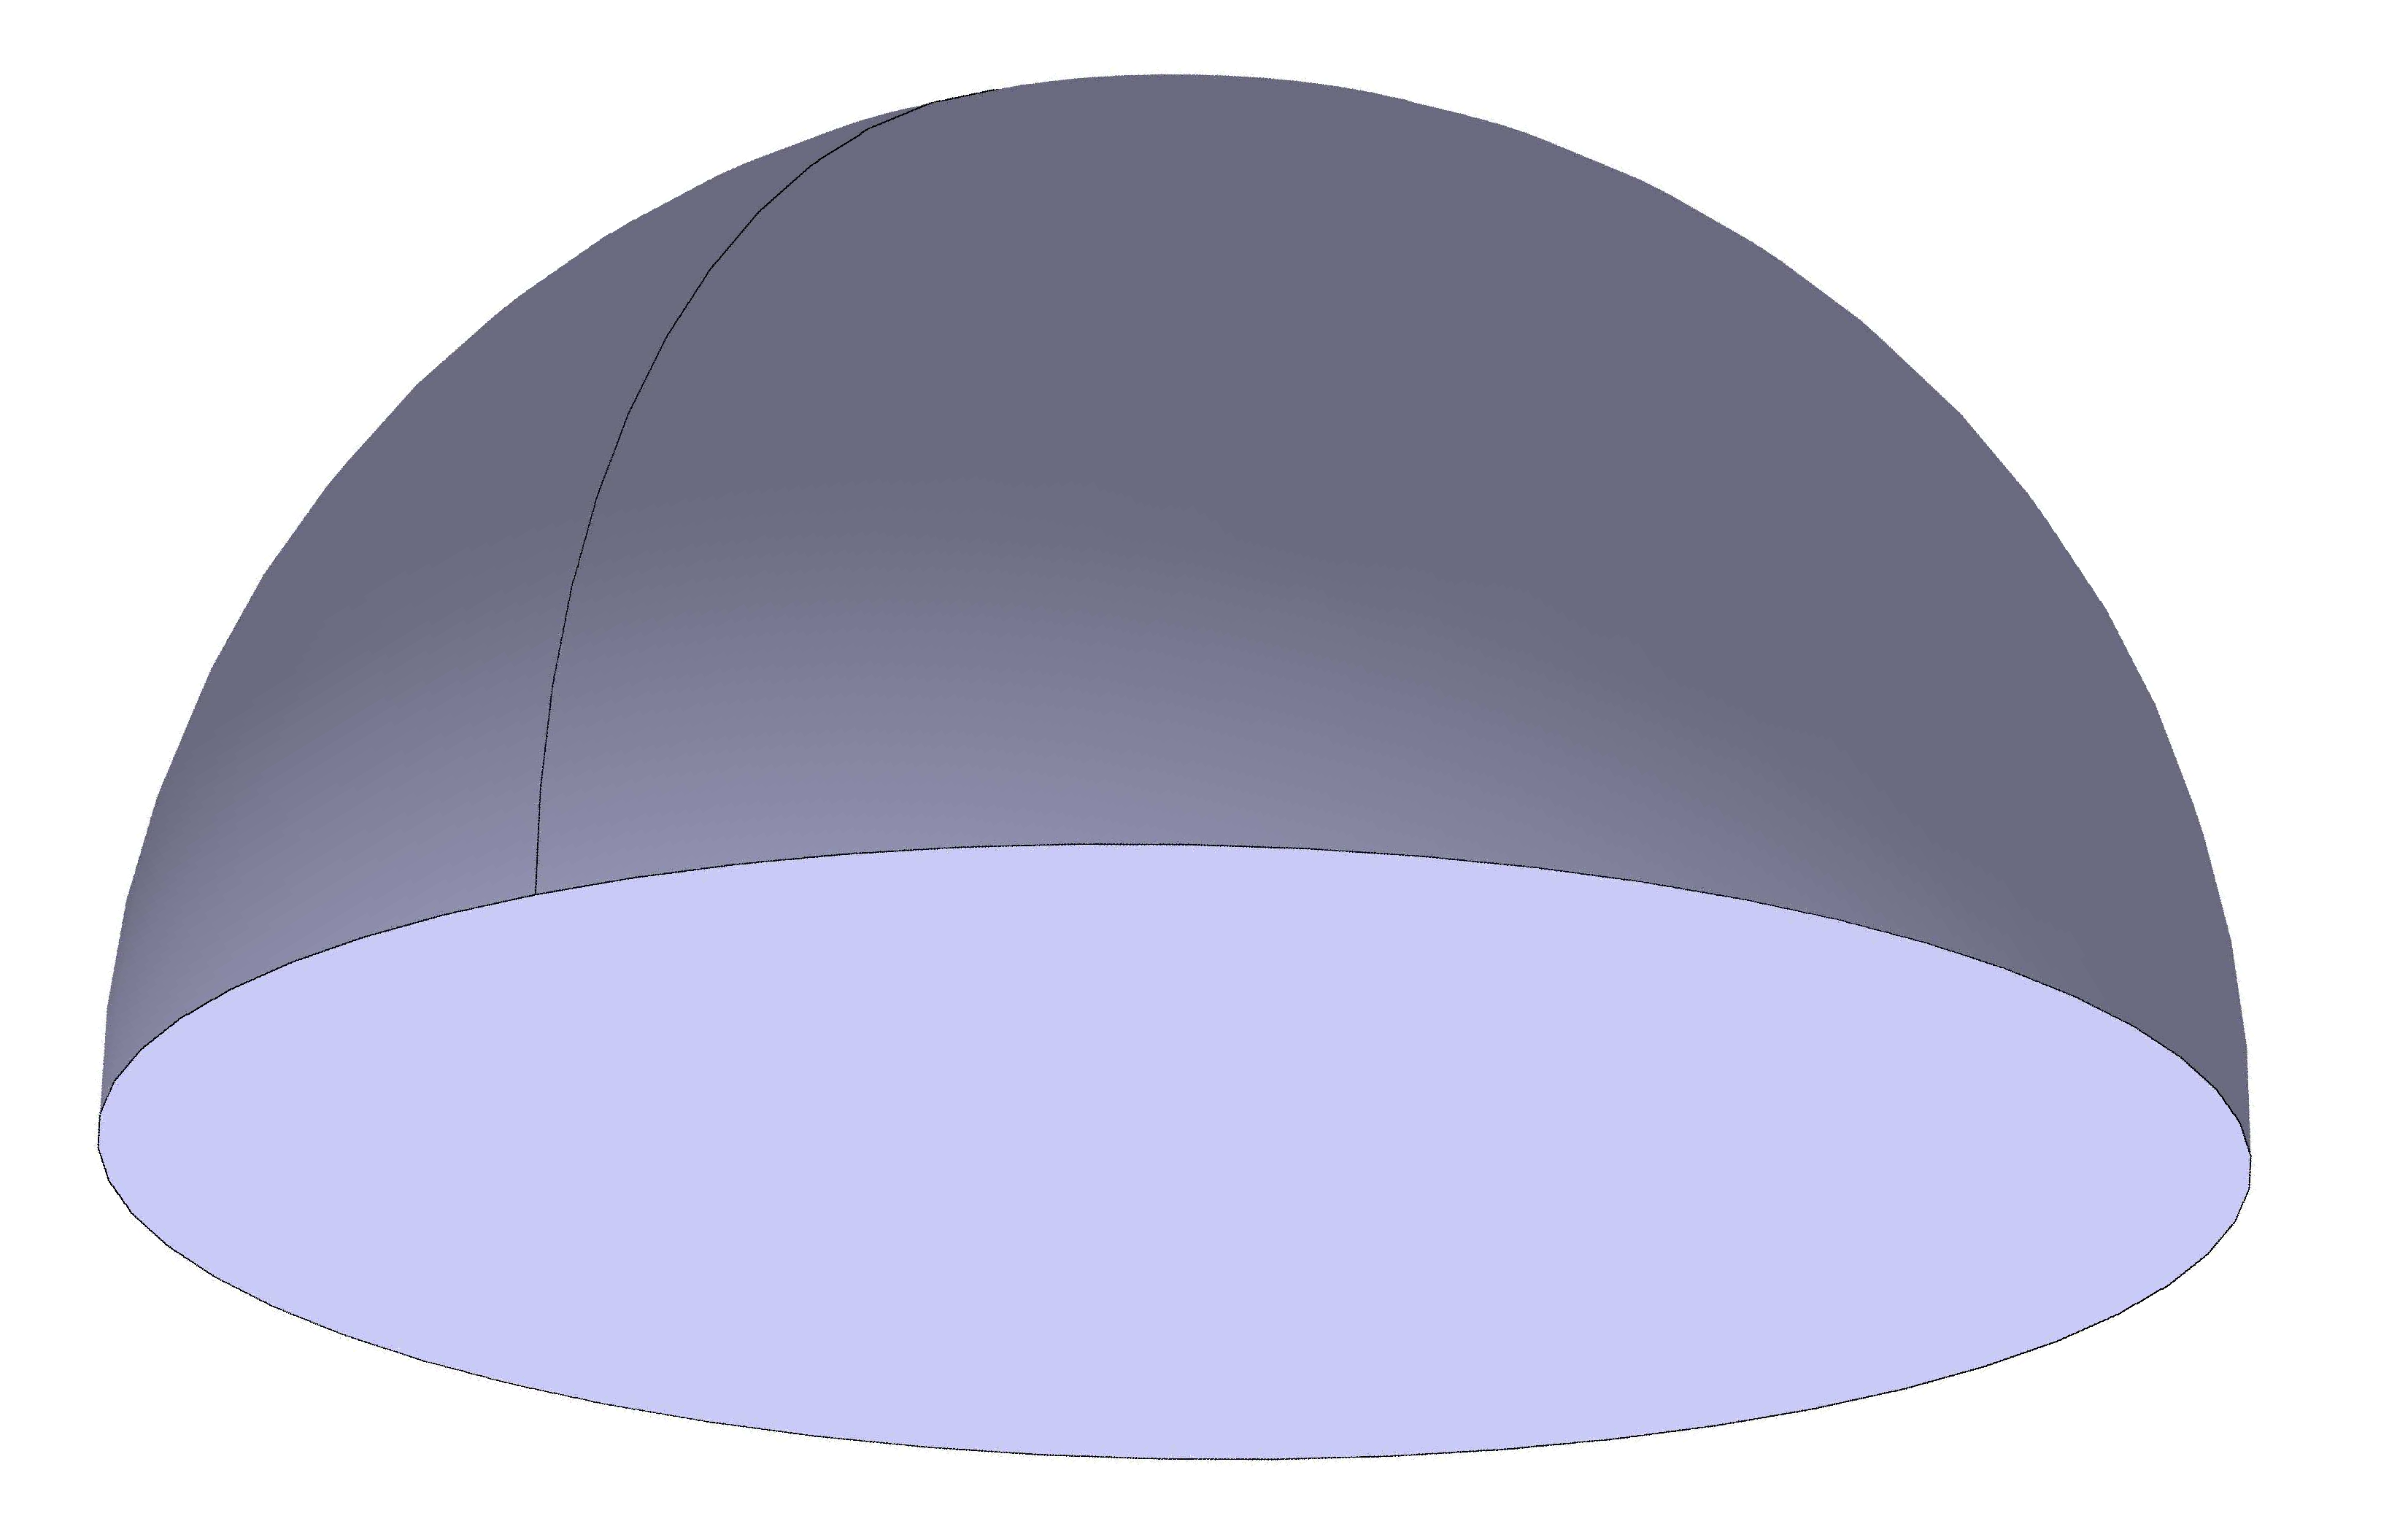
\includegraphics[width=1in]{Figures/Sphere3d}  & & 
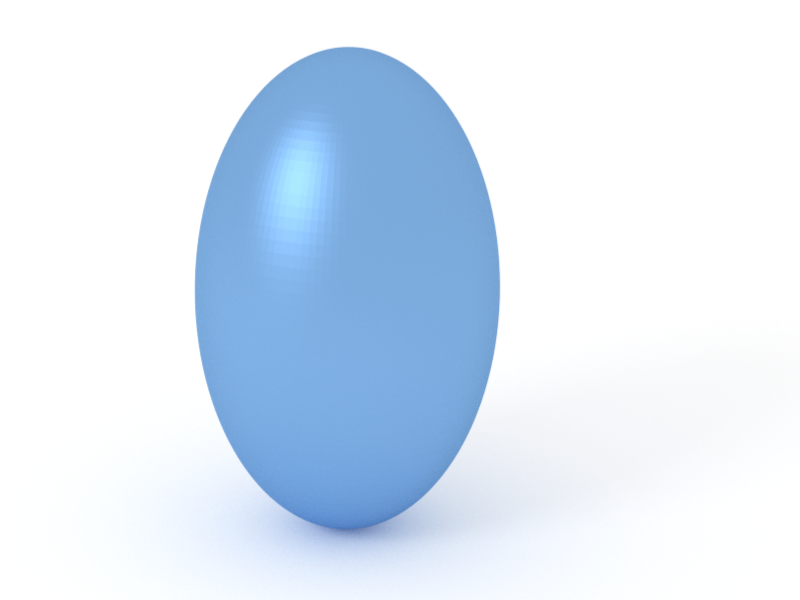
\includegraphics[width=1in]{Figures/FullSpheroid3d} & & 
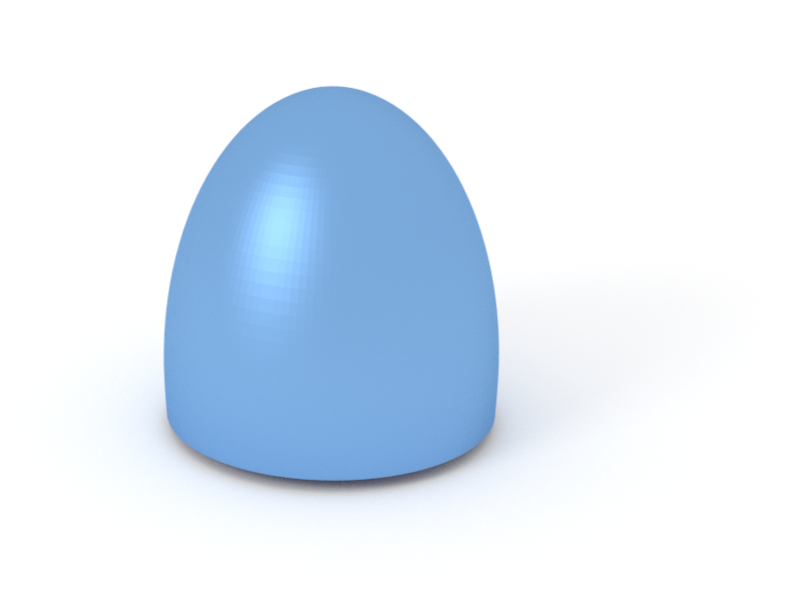
\includegraphics[width=1in]{Figures/Spheroid3d} & & 
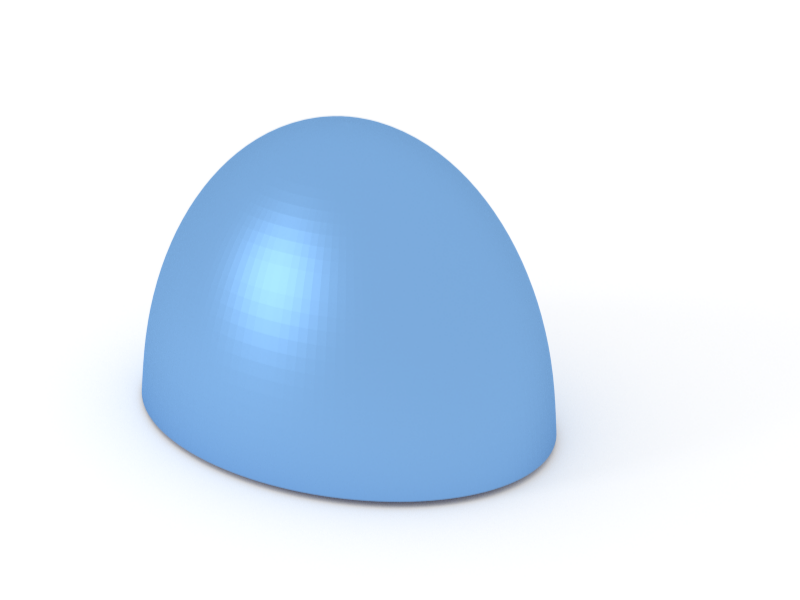
\includegraphics[width=1in]{Figures/HemiEllipsoid3d}\\
\hline
Ripple1, \SecRef{Ripple1} &  & Ripple2, \SecRef{Ripple2}& &   & &  \\
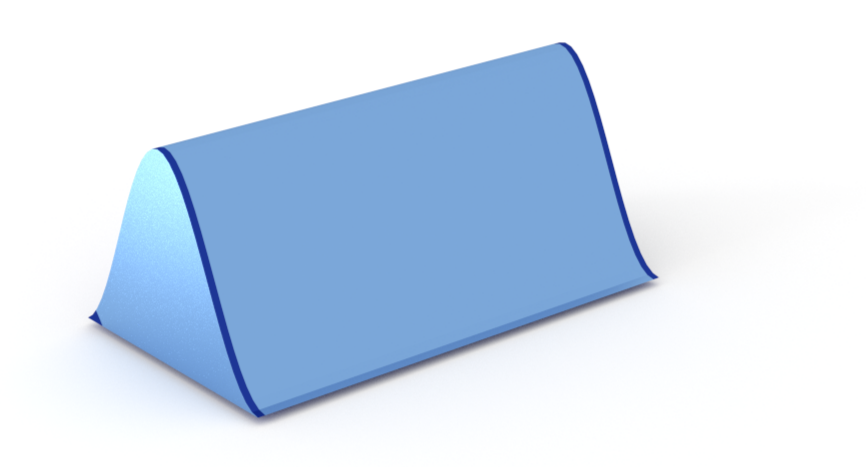
\includegraphics[width=1in]{Figures/Ripple13d} & & 
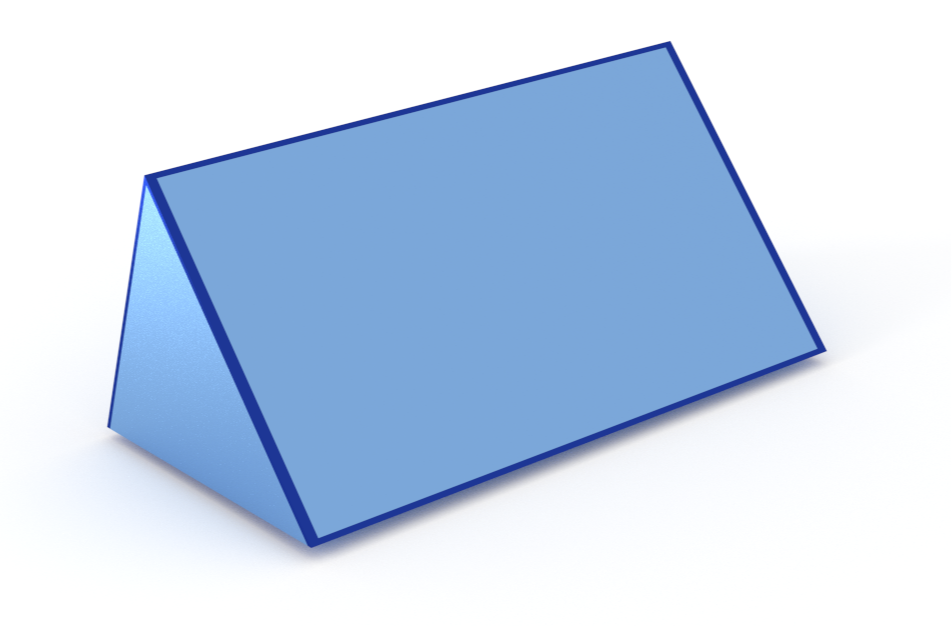
\includegraphics[width=1in]{Figures/Ripple23d} & &  & & \\
\hline 
\end{tabulary}
\end{table}

\newpage

%%%%%%%%%%%%%%%%%%%%%%%%%%%%%%%%%%%%%%%%%%%%%%%%%%%%%%%%%%%%%%%%%%%%%%%
\subsection{Distorted Wave Born Approximation} \SecLabel{sect:dwba}

Born approximation fails when multiple reflections and refractions have to be taken into account at interfaces because of the presence of underlying layers of materials and the closeness of  the incident angle $\alpha_i$ to the critical angle of total external reflection $\alpha_c$. The first order correction to the scattering theory is the Distorted Wave Born Approximation (DWBA), whereas the Born approximation is the zeroth order. \\
The collective effects between the particles are not considered in this section. They have been described in~\SecRef{sect:interf}.  We also do not take any polarization effects into account. They will be described in...\\

 In the DWBA, the form factor of a particle in a multilayer system is given by

\begin{align}
F_{\rm{DWBA}} (\vect{k}_i,\vect{k}_f, r_z) & = T_i T_f F_{\rm{BA}} (\vect{k}_i-\vect{k}_f) e^{i (k_{i,z}-k_{f,z}) r_z} + R_i T_f F_{\rm{BA}}(\vect{\widetilde{k}}_i-\vect{k}_f) e^{i(-k_{i,z}-k_{f,z})r_z}
 \nonumber \\
  &+ T_i R_f F_{\rm{BA}}(\vect{k}_i-\vect{\widetilde{k}}_f)e^{i(k_{i,z}+k_{f,z})r_z} + R_iR_fF_{\rm{BA}} (\vect{\widetilde{k}}_i-\vect{\widetilde{k}}_f)e^{i(-k_{i,z}+k_{f,z})r_z} \; , \label{eq:dwbageneral}
\end{align}
where $F_{\rm{BA}}$ is the expression of the form factor in the Born approximation, $r_z$ is the $z$-coordinate of the particle's position (measured from the bottom of the particle), $\vect{k}_i=(k_{i,x}, k_{i,y}, k_{i,z})$ $\vect{k}_f=(k_{f,x}, k_{f,y}, k_{f,z})$ are the incident and scattered wave vectors in air, respectively \cite{Raus95}. With a tilde (\~{}), these wavevectors components are evaluated in the multilayer system (the refractive indices of the different constituting materials have to be taken into account). 
$T_i$, $T_f$, $R_i$, $R_f$ are the transmission and reflection coefficients for the incident wave (index $i$) or the scattered one (index $f$). These coefficients can be calculated using the Parratt formalism \cite{Parr54} or the matrix method \cite{BoWo99}. $\vect{k}_i-\vect{k}_f$ is equal to the scattering vector $\vect{q}$ and the $z$-axis is pointing upwards.\\

\ImportantPoint{Remark:}{The particles cannot sit in between layers. At most they can be sitting on any inner interfaces.}

\vspace{18pt}

In the followings, the DWBA will be illustrated for two different layouts of particles: 
\begin{itemize}
\item particles deposited on a substrate,
\item particles buried in a layer on a substrate.
\end{itemize}

\ImportantPoint{Remark:}{In \BornAgain\ there is no limitation to the number of layers composing the sample.}

%%%%%%%%%%%%%%%%%%%%%%%%%%%%%%%%%%%%%%
\subsubsection{Particles deposited on a substrate}
%Substrate modified Born approximation
In this configuration, the particles are sitting on top of a substrate layer, in the air as shown in fig.~\ref{fig:SchemDWBA}. In the DWBA the expression of a form factor becomes 
\begin{align}
F_{\rm{DWBA}}(q_{\parallel}, k_{i,z}, k_{f,z}) &= F_{\rm{BA}}(q_{\parallel}, k_{i,z}-k_{f,z})+ R_i F_{\rm{BA}}(q_{\parallel}, -k_{i,z}-k_{f,z}) \nonumber \\
&+ R_f F_{\rm{BA}}(q_{\parallel}, k_{i,z}+k_{f,z}) + R_i R_f F_{\rm{BA}}(q_{\parallel},-k_{i,z}+k_{f,z}), \label{eq:dwbaair}
\end{align}
where $q_{\parallel}$ is the component of the scattering beam in the plane of the interface ($\vect{q}=\vect{k}_i-\vect{k}_f$), $k_{i,z}$ and $k_{f,z}$ are the z-component of the incident and scattered beam, respectively. $R_i$, $R_f$ are the reflection coefficients in incidence and reflection. They are defined as\\ $R=\dfrac{k_z+\sqrt{n_s^2k_0^2-|k_{\parallel}|^2}}{k_z-\sqrt{n_s^2 k_0^2-|k_{\parallel}|^2}}$, where $n_s=1-\delta_s -i \beta_s$ is the refractive index of the substrate, $k_0$ is the wavelength in vacuum ($2\pi /\lambda$), $k_z$ and $k_{\parallel}$ are the $z$-component and the in-plane component of $\vect{k}_i$ or $\vect{k}_f$. \\

\ImportantPoint{Remark:}{If the particles are sitting on a multilayered system, the expression of the form factor in the DWBA is obtained by replacing the Fresnel coefficient by the corresponding coefficients of the underlying layers \cite{Parr54,BoWo99}.}

\vspace{18pt}

Figure~\ref{fig:SchemDWBA} illustrates the four scattering processes for a supported particle, taken into account in the DWBA. The first term of eq.~\ref{eq:dwbaair}  corresponds to the Born approximation. Each term of $F_{\rm{DWBA}}$ is weighted by a Fresnel coefficient. 

\begin{figure}[h]
\begin{center}
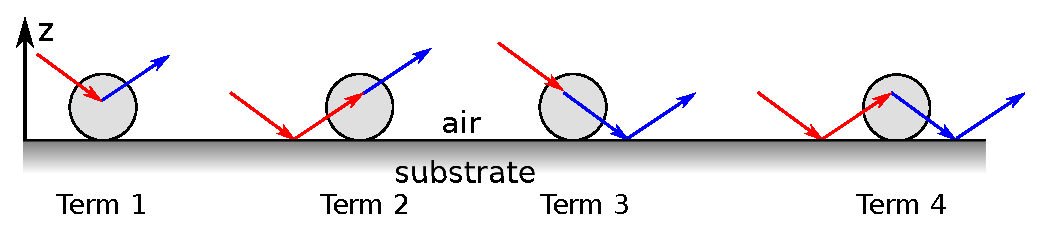
\includegraphics[width=\textwidth]{Figures/drawingDWBA}
\end{center}
\caption{Schematic views of the different terms appearing in the expression of the form factor under DWBA for particles sitting on a substrate layer.}
\label{fig:SchemDWBA}
\end{figure}


Script~\ref{lst:badwba} illustrates the difference between BA and DWBA in \BornAgain\ when generating the sample.  We consider the simple case of:
\begin{itemize}
\item one kind of particles' shape,
\item no interference between the particles,
\item in the DWBA, a sample made of a layer of substrate on which are deposited the particles,
\item in the BA, a sample composed of the particles in air.
\end{itemize} 

Figure~\ref{fig:spheroidbadwba} shows the intensity contourplot generated using this script with truncated spheroids as particles. Note that the full \Python\ script UMFormFactorBA\_DWBA.py is available in /Examples/Python/UserManual/.

\newpage


\begin{lstlisting}[language=python, style=eclipseboxed,numbers=none,nolol,caption={\Code{Python} script to generate a sample using Born or Distorted Wave Born Approximation. The difference between BA and DWBA in this simple case is the absence or presence of a substrate layer in the sample.},label={lst:badwba}]
def get_sample():
    """
    Build and return the sample to calculate form factor of 
    truncated spheroid in Born or Distorted Wave Born Approximation.
    """
    # defining materials
    m_ambience = HomogeneousMaterial("Air", 0.0, 0.0)
    m_substrate = HomogeneousMaterial("Substrate", 6e-6, 2e-8)
    m_particle = HomogeneousMaterial("Particle", 6e-4, 2e-8)

    # collection of particles
    ff= FormFactorTruncatedSpheroid(7.5*nanometer, 9.0*nanometer, 1.2)
    particleshape = Particle(m_particle, ff)
    particle_layout = ParticleLayout()
    particle_layout.addParticle(particleshape, 0.0, 1.0)

    # interferences
    interference = InterferenceFunctionNone()
    particle_layout.addInterferenceFunction(interference)

    # assembling the sample
    air_layer = Layer(m_ambience)
    air_layer.setLayout(particle_layout)
    substrate_layer = Layer(m_substrate, 0)

    multi_layer = MultiLayer()
    multi_layer.addLayer(air_layer)
    # Comment the following line out for Born Approximation
    multi_layer.addLayer(substrate_layer)
    return multi_layer
\end{lstlisting}


\begin{figure}[ht]
\hfill
\subfigure[Born Approximation]{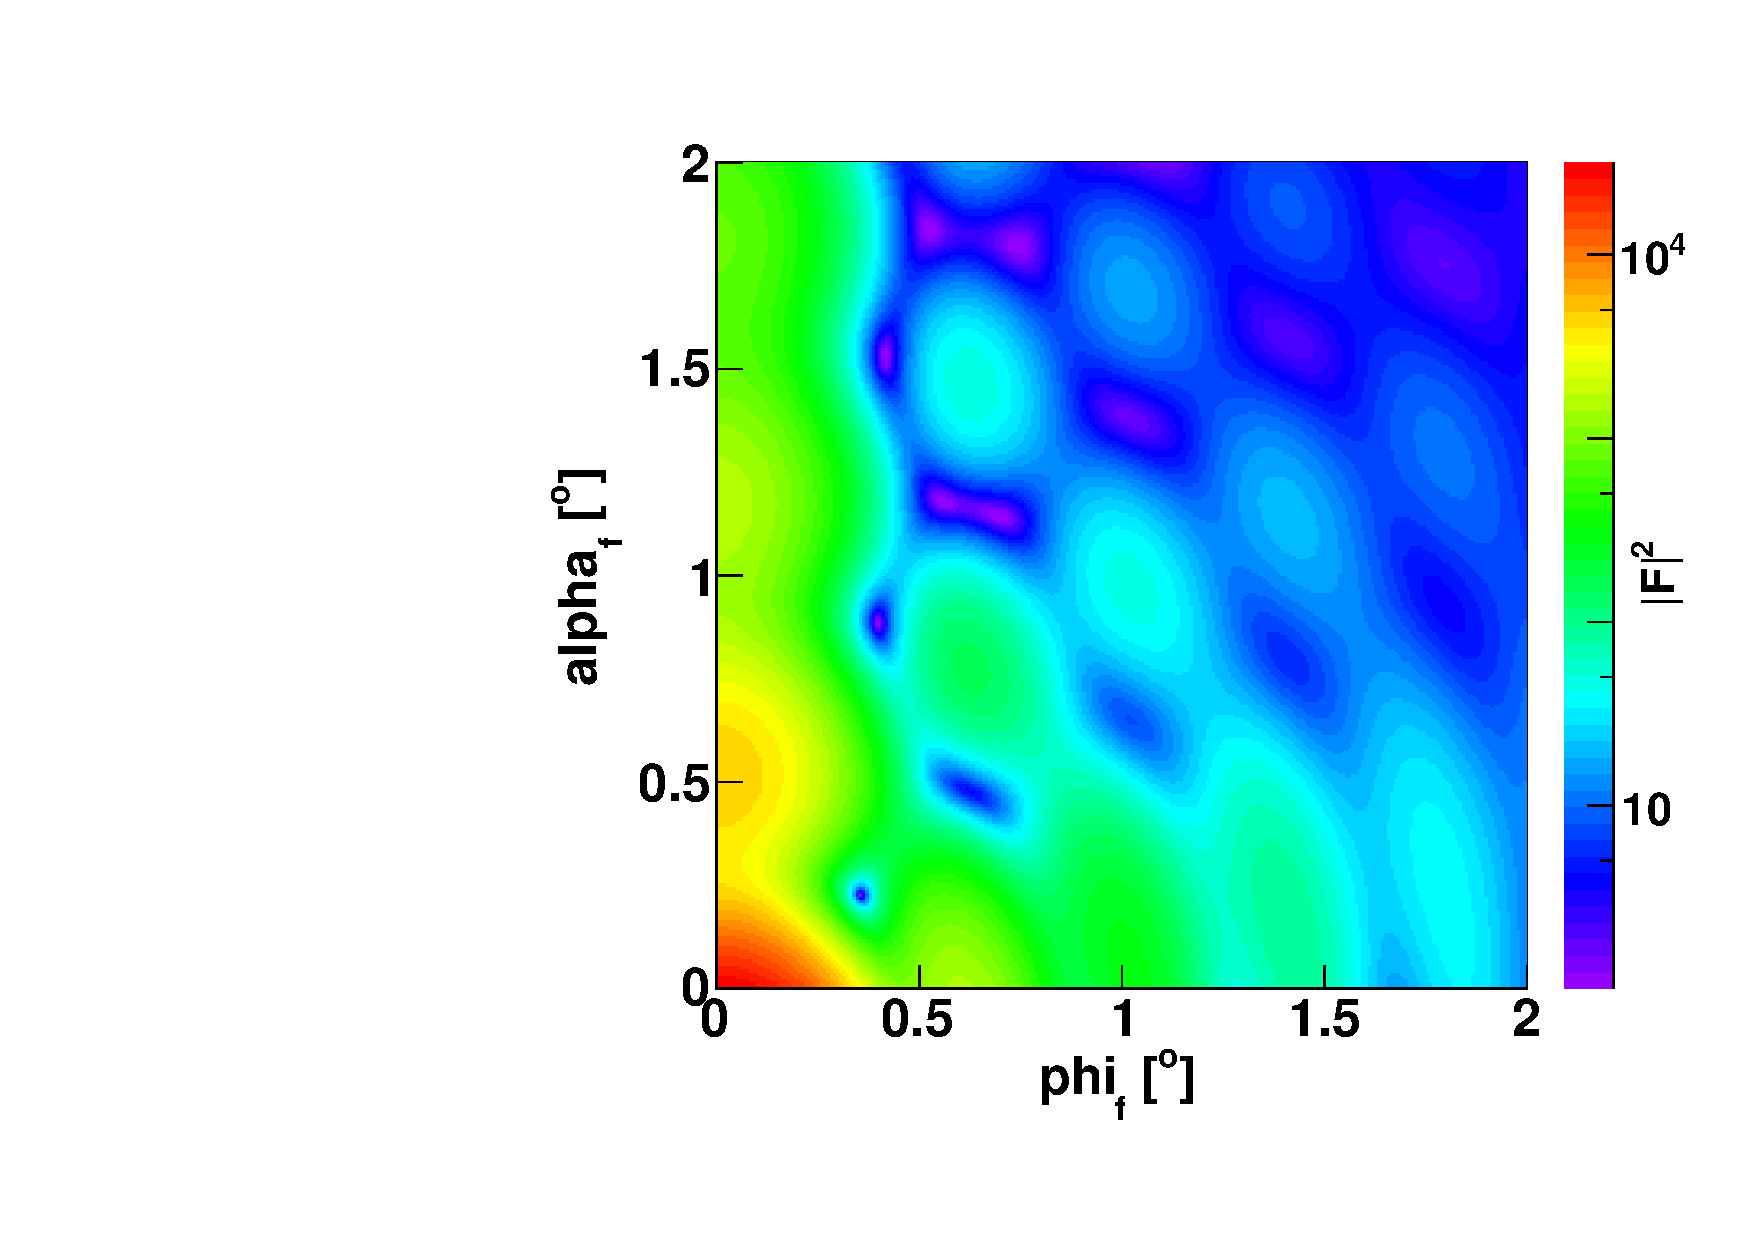
\includegraphics[width=6cm]{Figures/ffspheroidBA}}
\hfill
\subfigure[DWB Approximation]{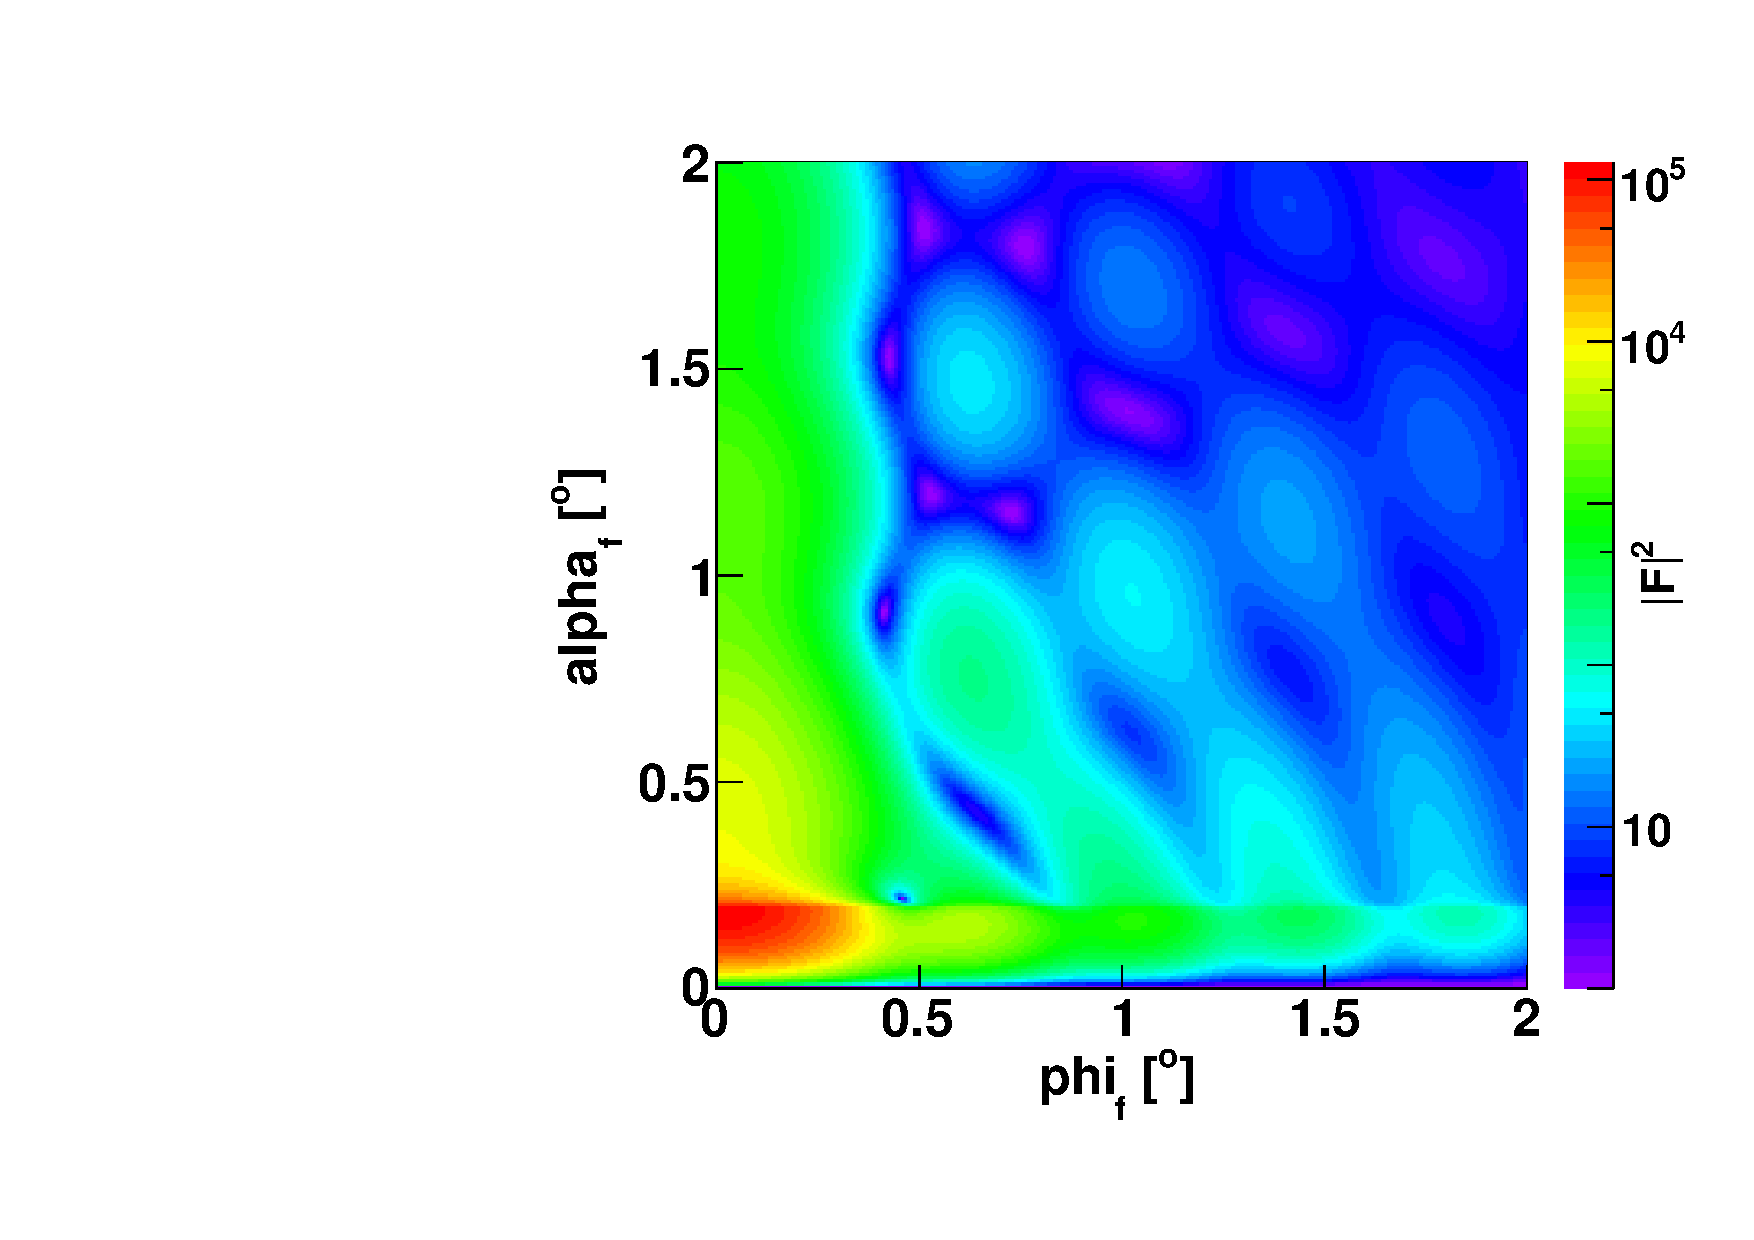
\includegraphics[width=6cm]{Figures/ffspheroidDWBA}}
\hfill
\caption{Intensity map of TruncatedSpheroid form factor in BA and DWBA computing using script~\ref{lst:badwba} for the sample.}
\label{fig:spheroidbadwba}
\end{figure}

\FloatBarrier 

\ImportantPoint{Remark:}{In \BornAgain, the DWBA is implemented automatically when assembling the sample with more than the air layer.}

\subsubsection{Buried particles} 

The system considered in this section consists of particles encapsulated in a layer, which is sitting on a substrate (see fig.~\ref{fig:SchemDWBAburied}). In this case the form factor in the DWBA is given by

\begin{align}
F_{\rm{DWBA}}(q_{\parallel}, k_{i,z}, k_{f,z}) &= T_i T_f F_{\rm{BA}}(q_{\parallel}, k_{i,z}-k_{f,z})e^{i(k_{i,z}-k_{f,z})d}+ R_i T_f F_{\rm{BA}}(q_{\parallel}, -k_{i,z}-k_{f,z})e^{i(-k_{i,z}-k_{f,z})d} \nonumber \\
&+ R_f T_i F_{\rm{BA}}(q_{\parallel}, k_{i,z}+k_{f,z}) e^{i(k_{i,z}+k_{f,z})d}+ R_f R_iF_{\rm{BA}}(q_{\parallel},-k_{i,z}+k_{f,z})e^{i(-k_{i,z}+k_{f,z})d}, \label{eq:dwbaburied}
\end{align}

\begin{equation*}
R_j =\frac{t^{j}_{0,1}r^{j}_{1,2}\exp(2ik_{j,z}t)}{1+r^{j}_{0,1}r^{j}_{1,2}\exp(2ik_{j,z}t)}, \quad T_j=\frac{t^{j}_{0,1}}{1+r^{j}_{0,1}r^{j}_{1,2}\exp(2ik_{j,z}t)}, j=i,f 
\end{equation*}
where $q_{\parallel}$ is the component of the scattering beam in the plane of the interface, $k_{i,z}$ and $k_{f,z}$ are the z-component of the incident and scattered beams, respectively.  $d$ is the depth at which the particles are sitting in the layer. Note that this value is given relative to the top of this layer and it is not the coordinate in the absolute referential (linked with the full sample) and it is measured up to the bottom of the particle. $t$ is the thickness of the intermediate layer containing the particles. $R_{i,f}$ and $T_{i,f}$  are the reflection  and transmission coefficients in incidence and reflection (they can be calculated using Parratt or matrix formalism). $r^j_{0,1}$, $r^j_{1,2}$ $t^j_{0,1}$ are the reflection and transmission coefficients between layers; the indices are related to different boundaries with 0: air, 1: intermediate layer and 2: substrate layer and the superscript $j$ is associated with the incident or scattered beams:
\begin{equation*}
r^j_{n,n+1}=\frac{k_{j,z,n}-k_{j,z,n+1}}{k_{j,z,n}-k_{j,z,n+1}}, \qquad t^j_{n,n+1}= \frac{2k_{j,z,n}}{k_{j,z,n}-k_{j,z,n+1}}, \quad n=0,1, \quad j=i,f,
\end{equation*}
where index $n$ is related to the layers, $z$ to the vertical component, and $j$ to the beams (incident and outgoing).

\begin{figure}[h]
\begin{center}
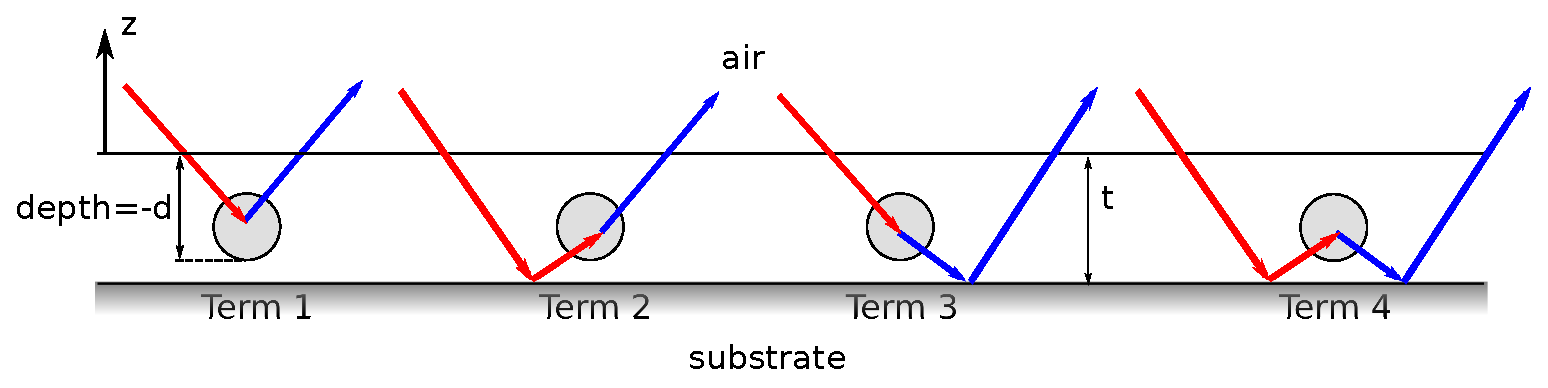
\includegraphics[width=\textwidth]{Figures/drawingDWBAburied}
\end{center}
\caption{Schematic views of the different terms appearing in the expression of the form factor under the DWBA for buried particles.}
\label{fig:SchemDWBAburied}
\end{figure}



Figure~\ref{fig:dwbaburied} shows a typical example of the output intensity scattered from a sample made of 3 layers: air, substrate, and in between, spherical particles embedded in the middle of a 30~nm-thick layer. This figure had been generated using listing~\ref{lst:dwbaburied} (The full script UMFormFactor\_Buried\_DWBA.py can be found in /Examples/Python/UserManual).

\begin{lstlisting}[language=python, style=eclipseboxed,numbers=none,nolol,caption={\Code{Python} script to generate a sample where spherical particles are embedded in the middle of a layer on a substrate.},label={lst:dwbaburied}]
def get_sample():
    """
    Build and return the sample with buried spheres in DWBA.
    """
    # defining materials
    m_ambience = HomogeneousMaterial("Air", 0.0, 0.0)
    m_interm_layer = HomogeneousMaterial("IntermLayer",3.45e-6, 5.24e-9)
    m_substrate = HomogeneousMaterial("Substrate", 7.43e-6, 1.72e-7)
    m_particle = HomogeneousMaterial("Particle", 0.0, 0.0)

    # collection of particles 
    ff = FormFactorFullSphere(10.2*nanometer)
    particleshape = Particle(m_particle, ff)
    particle_layout = ParticleLayout()
    particle_layout.addParticle(particleshape,20.1,1.0)

    # interferences 
    interference = InterferenceFunctionNone()
    particle_layout.addInterferenceFunction(interference)

    # assembling the sample 
    air_layer = Layer(m_ambience)
    intermediate_layer = Layer(m_interm_layer, 30.*nanometer)
    intermediate_layer.setLayout(particle_layout)
    substrate_layer = Layer(m_substrate, 0)
   
    multi_layer = MultiLayer()
    multi_layer.addLayer(air_layer)
    multi_layer.addLayer(intermediate_layer)
    multi_layer.addLayer(substrate_layer)
    return multi_layer
\end{lstlisting}


\begin{figure}[ht]
\centering
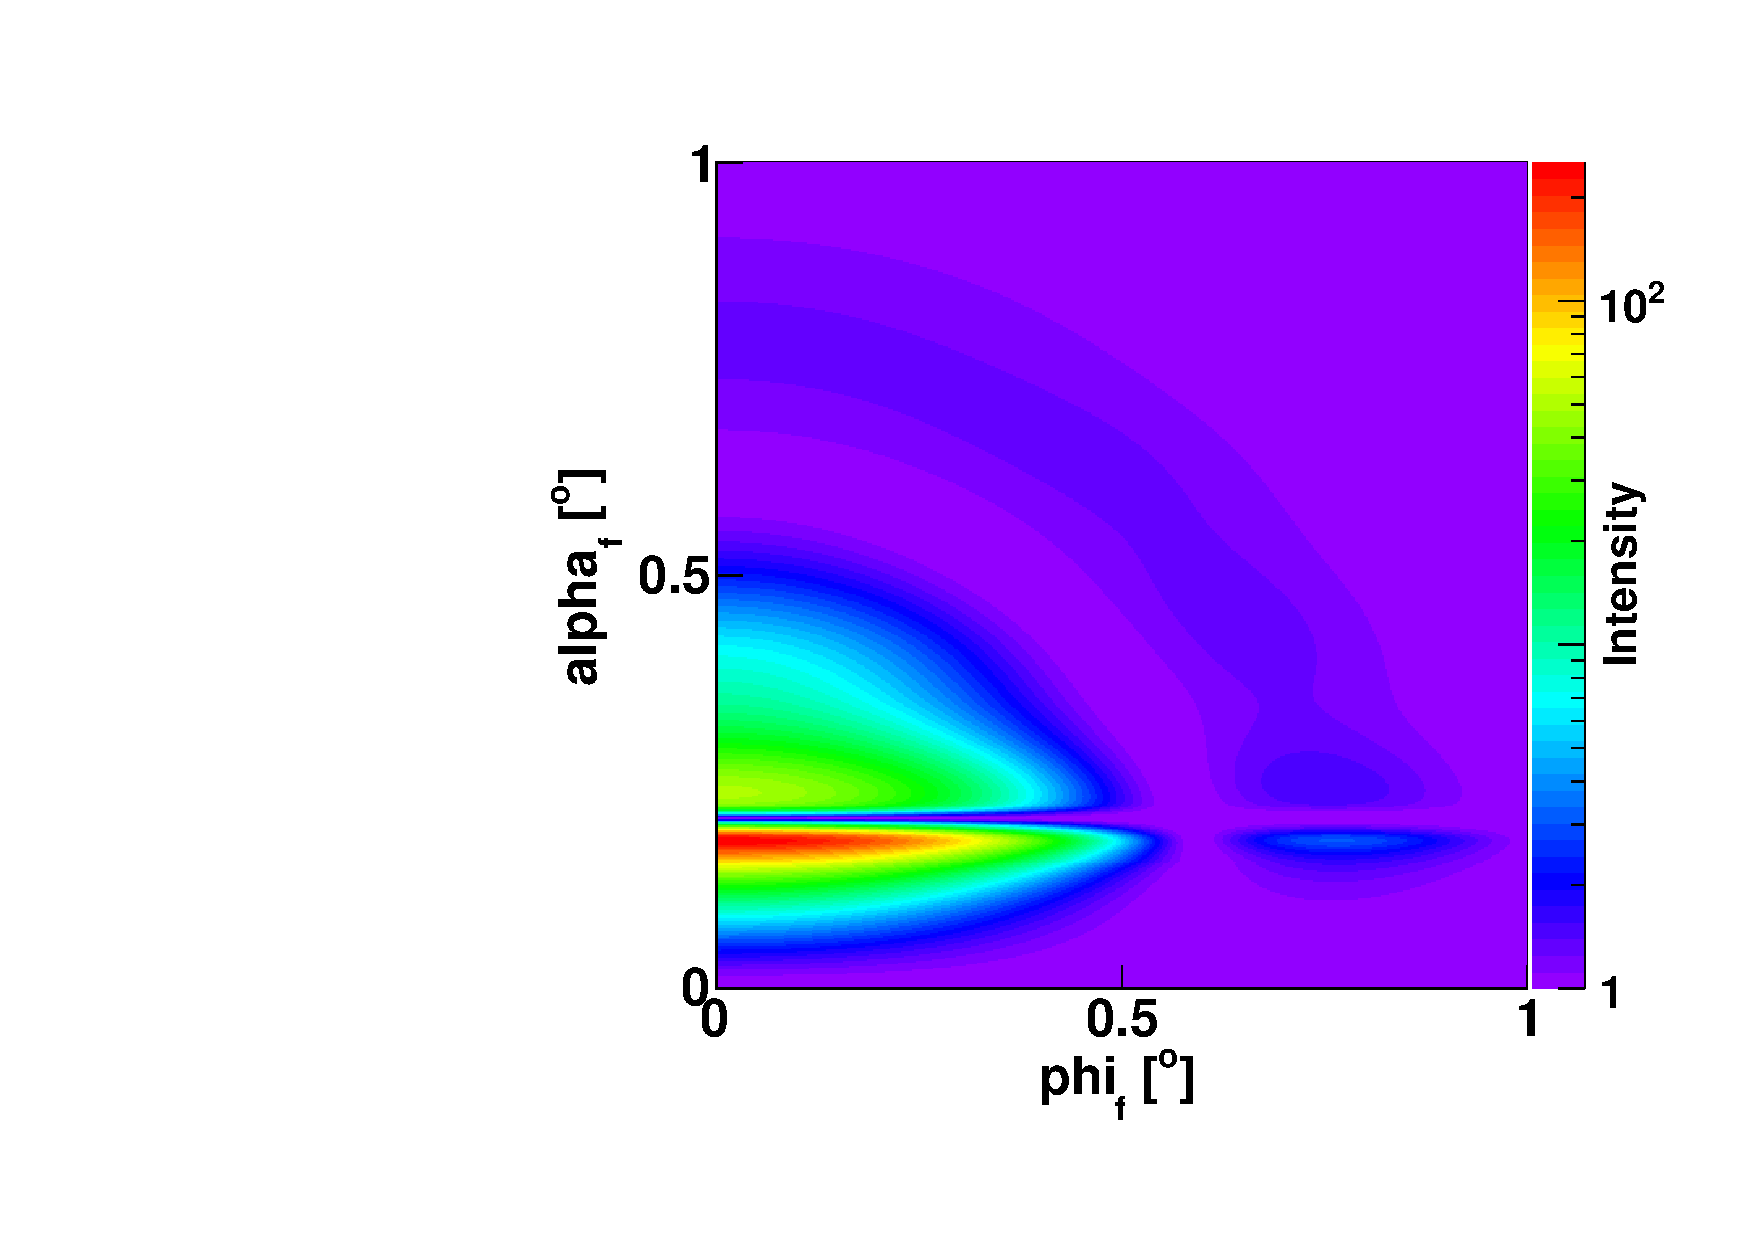
\includegraphics[width=0.6\textwidth]{Figures/figIntBuriedPart}
\caption{Map of intensity scattered from a sample made of spherical particles embedded in the middle of a 30~nm-thick layer on a substrate (see Script~\ref{lst:dwbaburied} for details about the sample).}
\label{fig:dwbaburied}
\end{figure}

\newpage

\ImportantPoint{Remark:}{For layers different from the air layer, the top interface is considered as the reference level to position the encapsulated particles. For example, spheres positioned at depth $d$ (positive) are located at a distance $d$ from the top of the layer up to the bottom of these particles. This convention is different for the top air layer, where particles sitting at the interface with an underlying layer (\textit{i.e.} the bottom of the air layer) are located at depth 0 (see fig.~\ref{fig:depthpartBA}).}


\begin{figure}[ht]
\centering
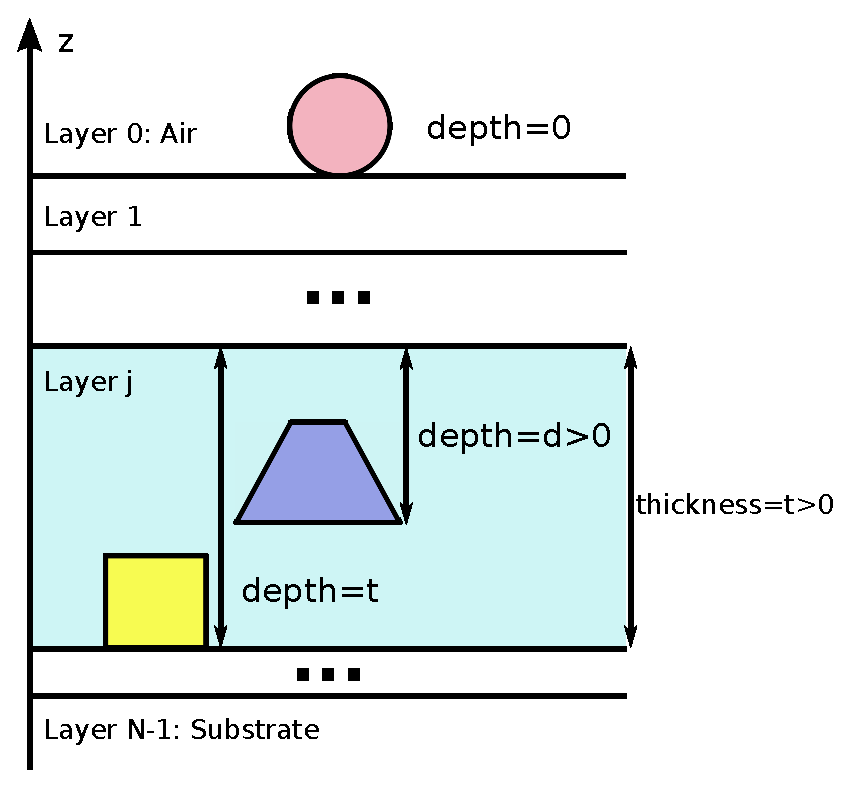
\includegraphics[width=0.5\textwidth]{Figures/drawingDepthParticle}
\caption{Illustration of the convention about \Code{depth} used in \BornAgain\ to encapsulate particles in layers.}
\label{fig:depthpartBA}
\end{figure}


\newpage
%%%%%%%%%%%%%%%%%%%%%%%%%%%%%%%%%%%%%%%%%
\section{More complicated particles' shapes} 
\BornAgain\ also offers the possibility to simulate more complicated shapes of particles by combining those listed in Table~\ref{tab:formfactors}. 

\subsection{Core-shell particles}
 To generate a core-shell particle, the combination is performed using the following command:\\
\Code{ParticleCoreShell(shell\_particle, core\_particle, relative\_core\_position)},\\
where \Code{shell\_particle} and \Code{core\_particle} are the outer and inner parts of the core-shell particle, respectively. They refer to one of the form factors defined previously and to an associated material. For example, for the outer part,\\ \Code{shell\_particle=Particle(material\_shell, outer\_form\_factor)},\\ where \Code{material\_shell} is the material of the shell and \Code{outer\_form\_factor} is the shape of the outer part (cf. listing~\ref{lst:cshellsample}). \\ \Code{relative\_core\_position} defines the position of the inner shape with respect to the outer one; it is defined with respect to the centre of the base of the particular form factor. An example in fig.~\ref{fig:coreshell} shows a core shell particle made of a box for the outer part and of a shifted pyramidal shape for the inner one.\\

Figure~\ref{fig:FFCoreShellBA} displays the output intensity scattered in the Born Approximation using the code listed in~\ref{lst:cshellsample} to generate the core-shell particle. The full script can be found at /Examples/python/UserManual/UMFormFactor\_CoreShell.py. 

\begin{figure}[ht]
\hfill
\subfigure[Side view]{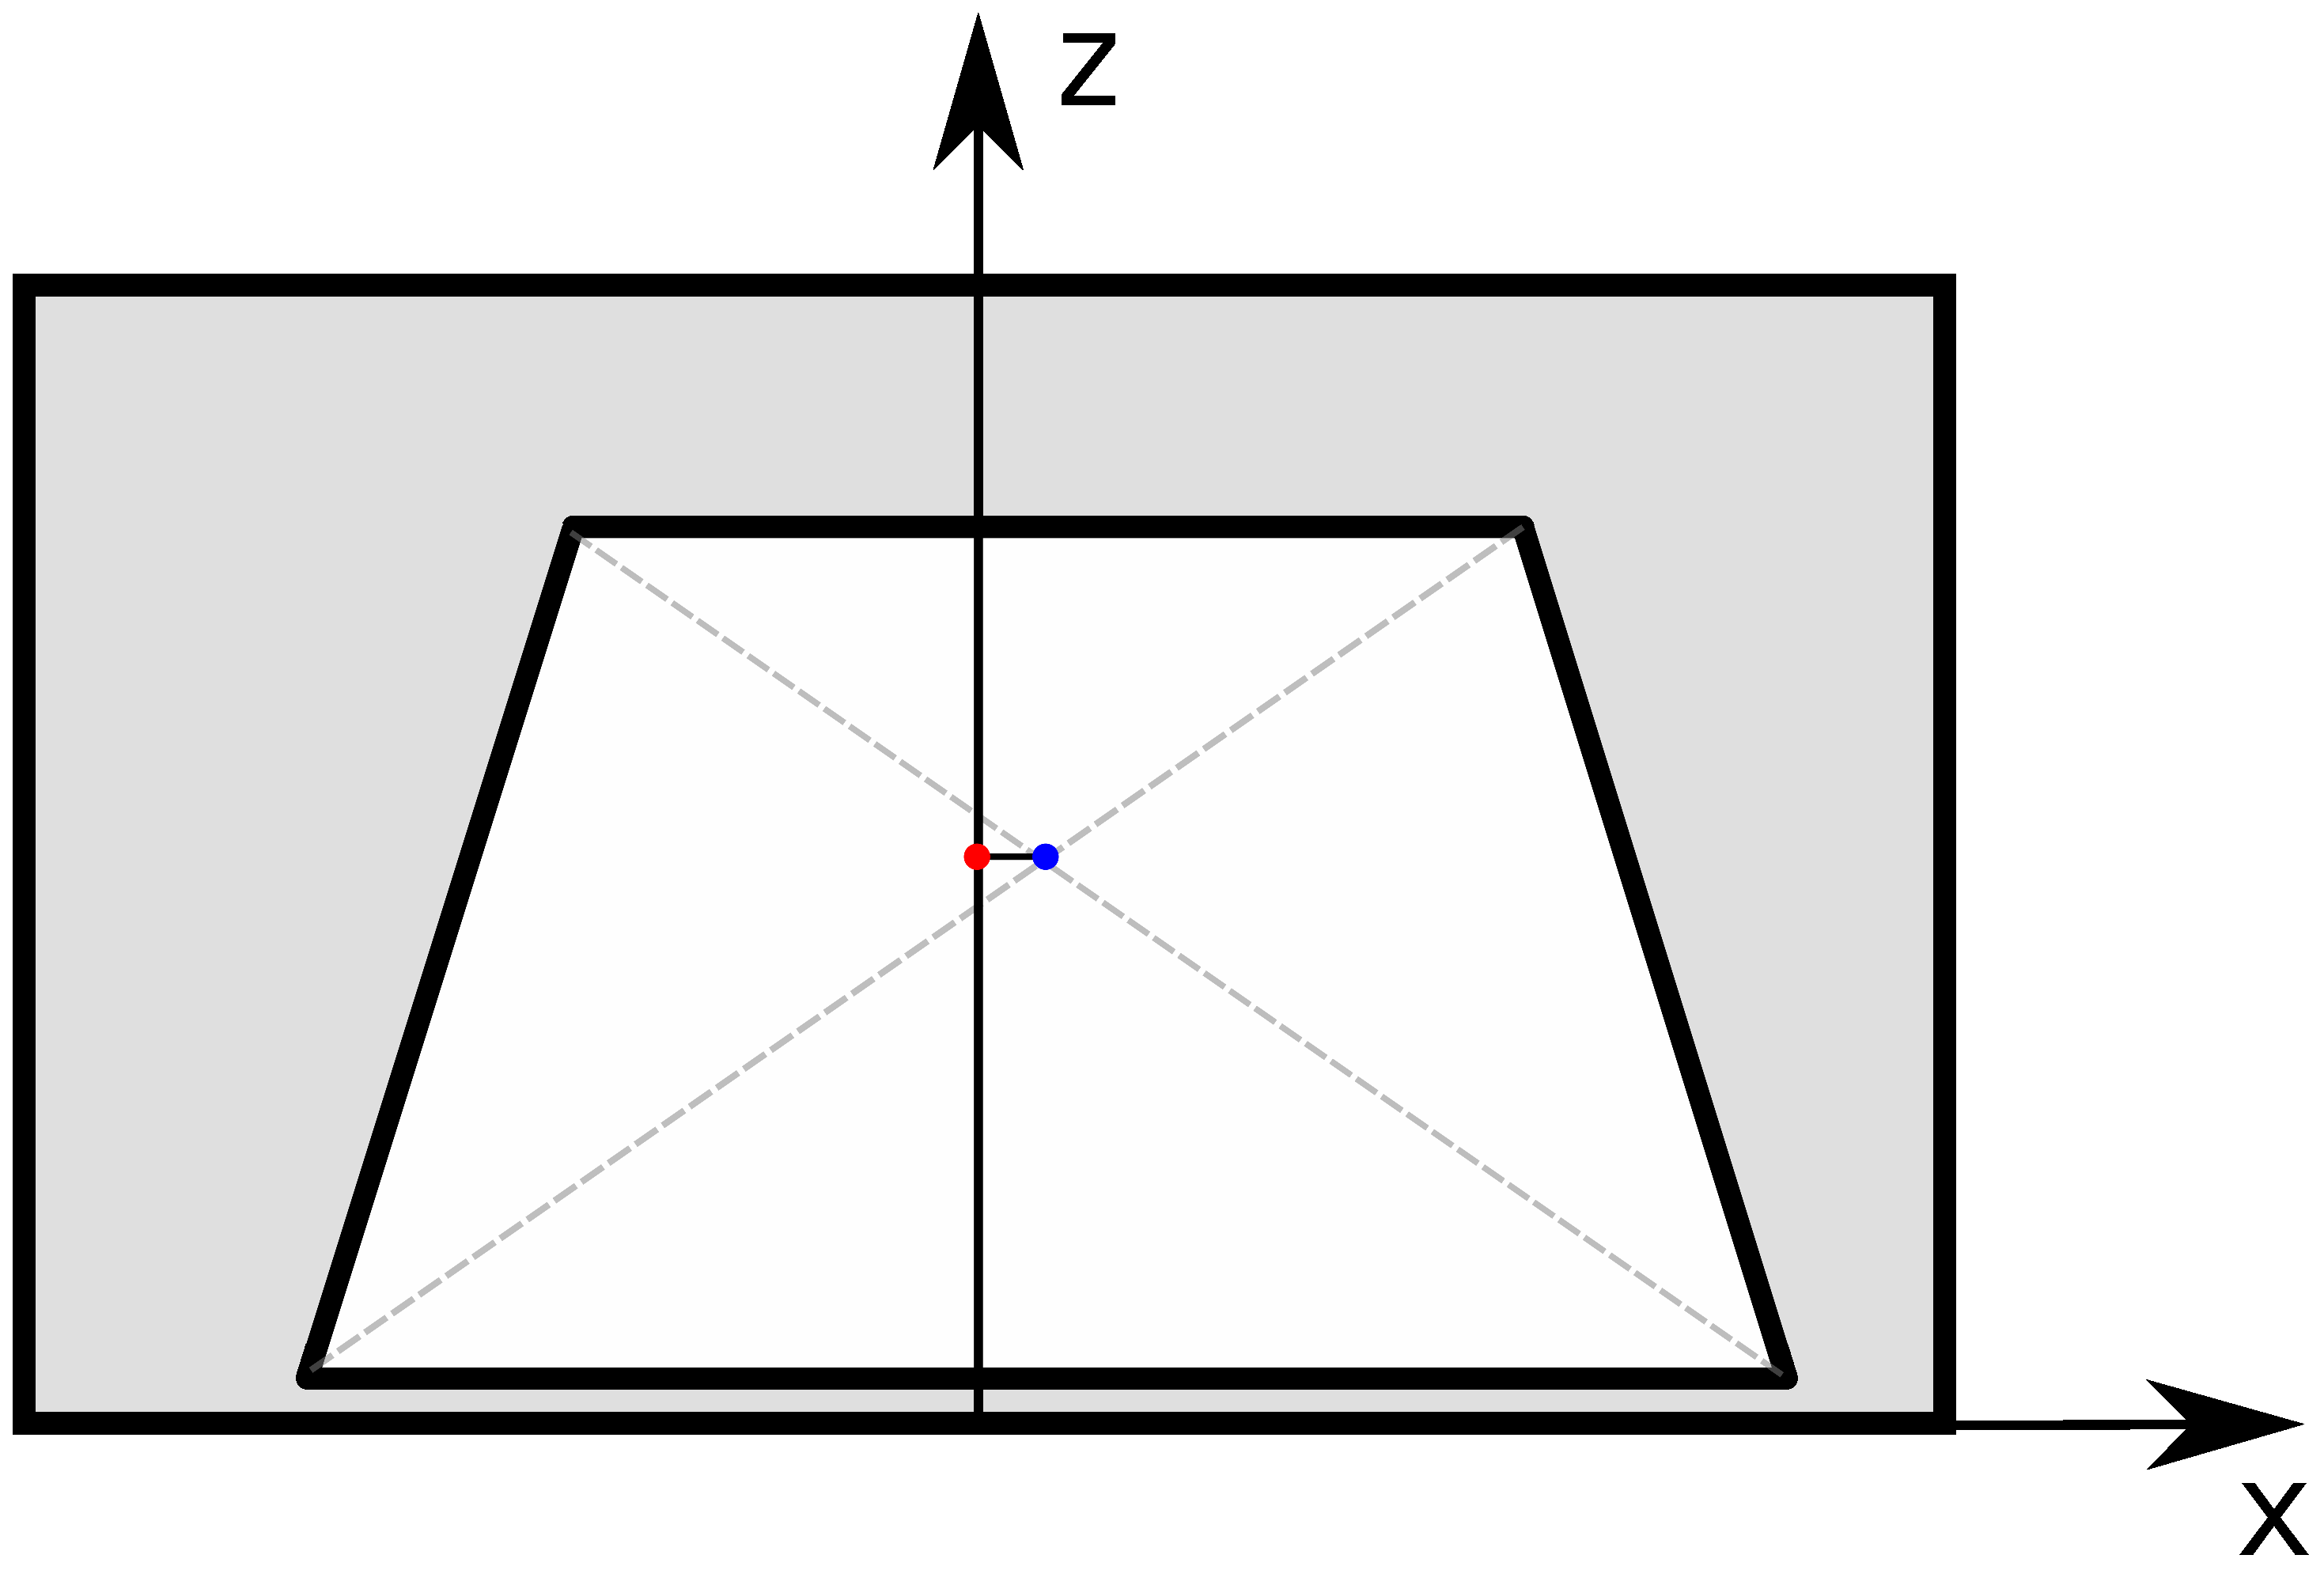
\includegraphics[width=5cm]{Figures/CoreShellParallPyrxz}}
\hfill
\subfigure[Top view]{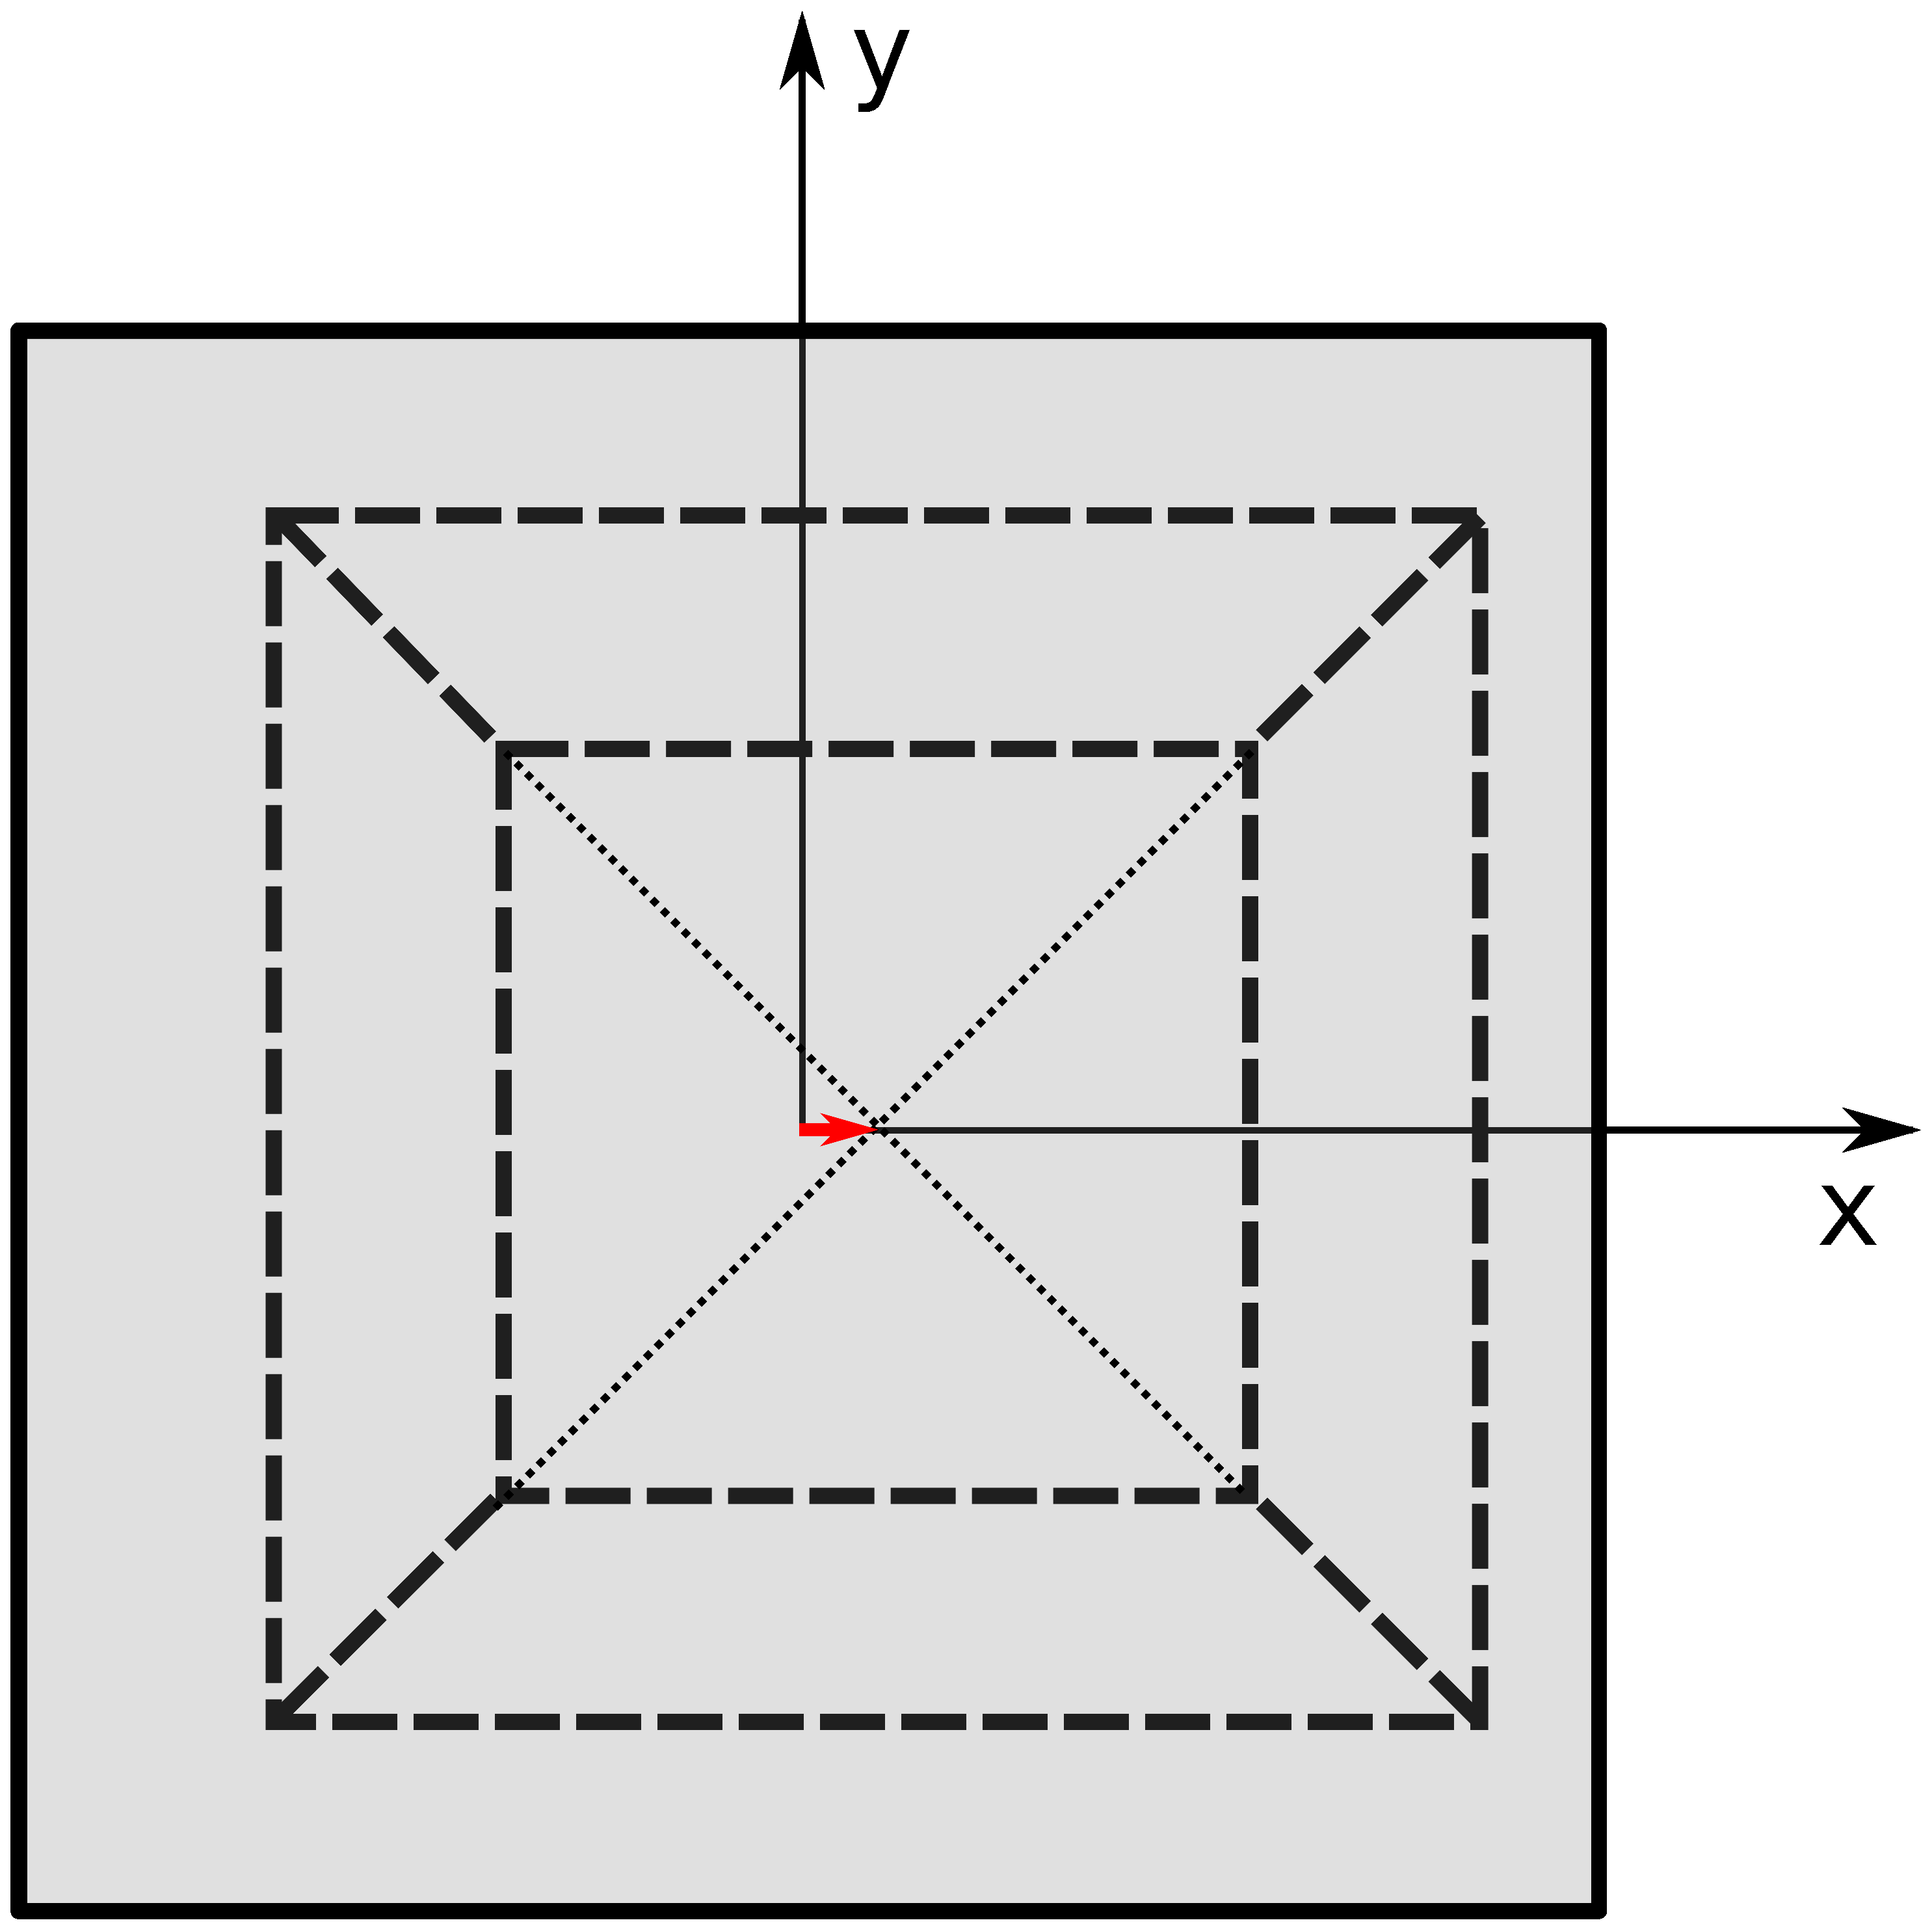
\includegraphics[width=5cm]{Figures/CoreShellParallPyrxy}}
\hfill
\caption{Example of a core-shell particle composed of a box with a pyramidal  inset. The relative core shell position is marked by the positions of the centres of the bases. }
\label{fig:coreshell}
\end{figure}

\newpage


\begin{lstlisting}[language=python,
  style=eclipseboxed,numbers=none,nolol,caption={\Code{Python} script
    to create a core-shell particle made of a box with a pyramidal shifted inset.},label={lst:cshellsample}]
    outer_ff = FormFactorBox(16.0*nanometer, 16.0*nanometer, 8.0*nanometer) 
    inner_ff = FormFactorPyramid(12.0*nanometer, 7.0*nanometer, 60.0*degree)
    shell_particle = Particle(m_shell, outer_ff)
    core_particle = Particle(m_core, inner_ff)
    core_position = kvector_t(1.5, 0.0, 0.0)

    particle = ParticleCoreShell(shell_particle, core_particle, core_position)
\end{lstlisting}

\begin{figure}[h]
\begin{center}
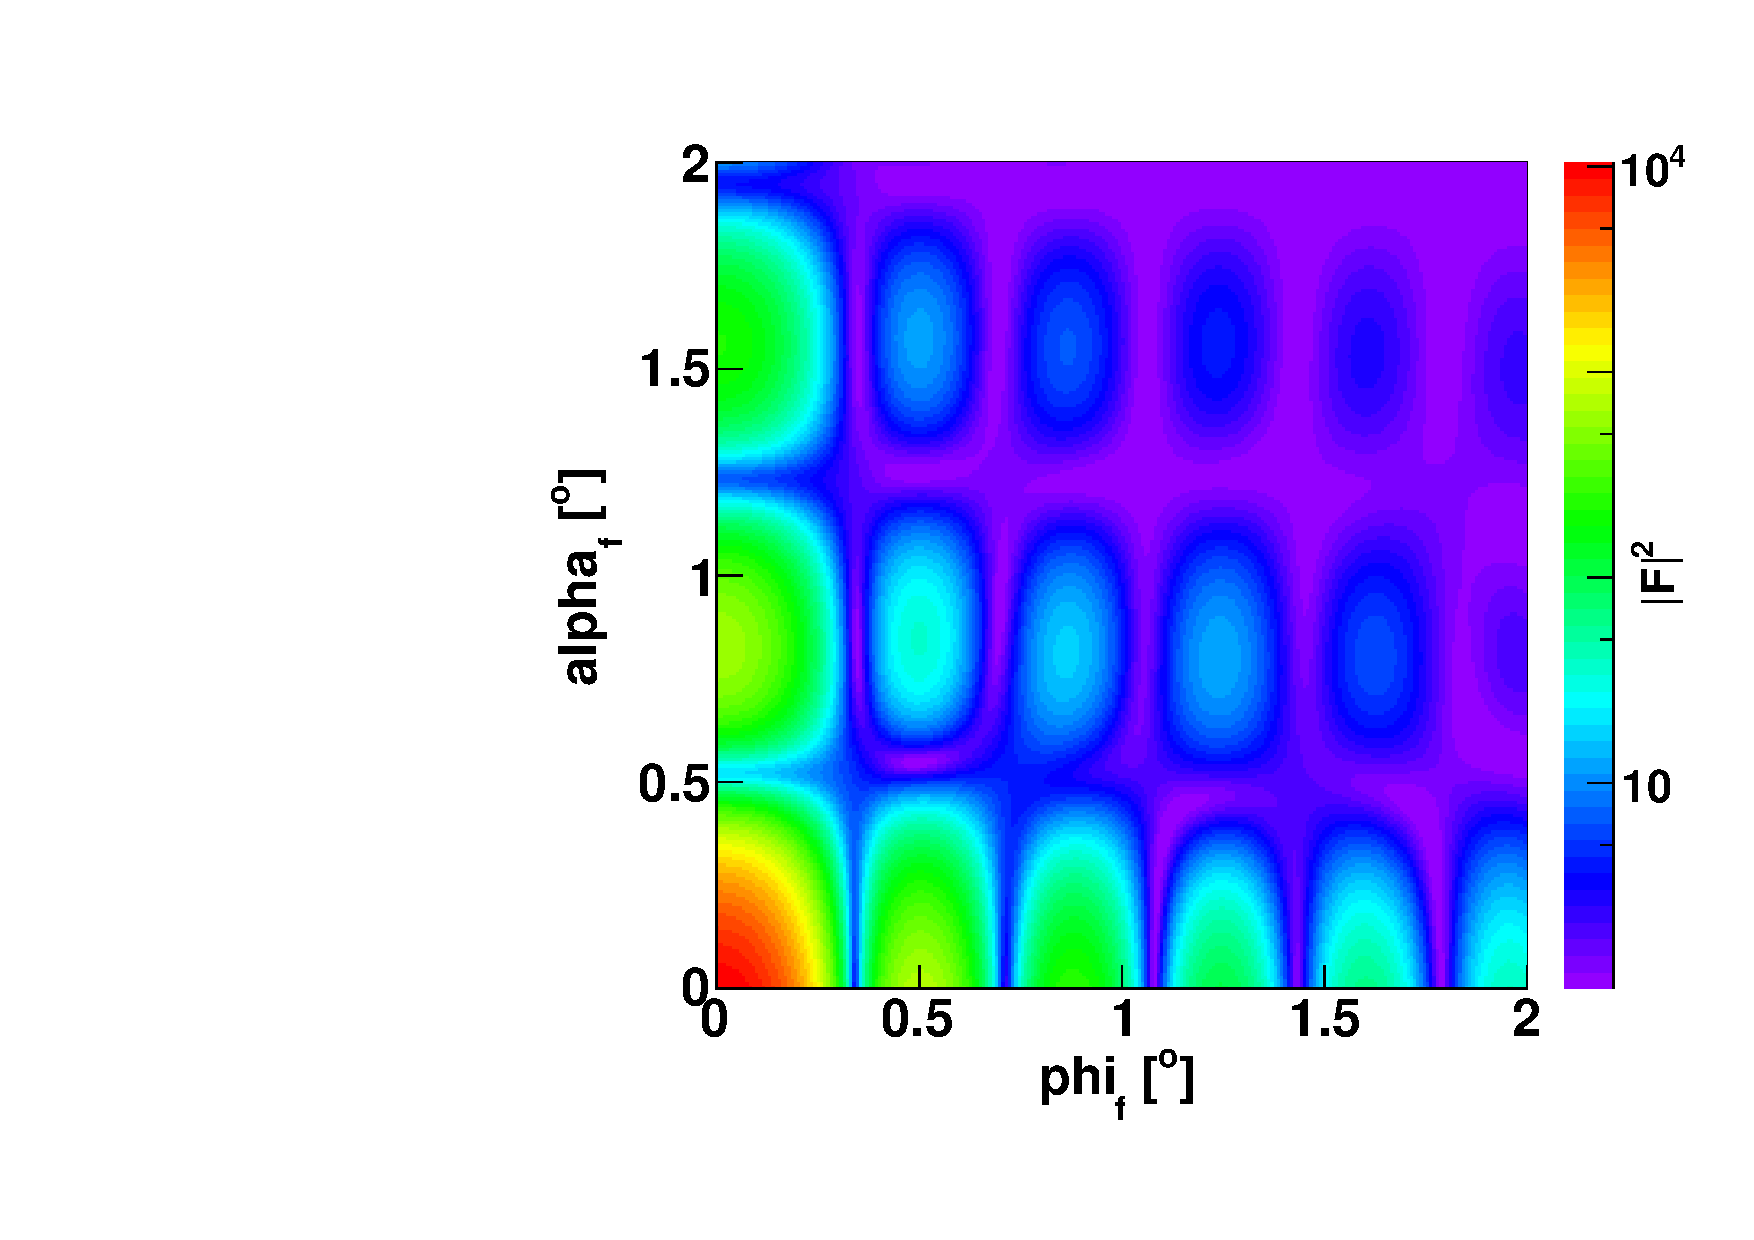
\includegraphics[width=0.6\textwidth]{Figures/CoreShellParallPyr}
\end{center}
\caption{Intensity map of a core-shell form factor in Born Approximation using  \Code{FormFactorBox(16*nanometer, 16*nanometer, 8*nanometer)} and \Code{FormFactorPyramid(12*nanometer, 7*nanometer, 60*degree)} for the outer and inner shells, respectively. The core particle is shifted by 1.5~nm in the $x$-direction with respect to the centre of the outer shell. The sample used to generate the particle is listed in~\ref{lst:cshellsample}.  There is no substrate and no interference between the particles.}
\label{fig:FFCoreShellBA}
\end{figure}

%%%%%%%%%%%%%%%%%%%%%%%%%%%%%%%%%%%%%%%%%
\subsection{Rotation of particles}

The particles can be rotated in a different direction by using one of
the following transformations: \Code{CreateRotateX($\theta$),
  CreateRotateY($\theta$), CreateRotateZ($\theta$)}, where capital X, Y, Z mark rotations
around the associated axis and $\theta$ is the
angle of rotation from this axis. For example, the following \Code{Python}\ script shows how to rotate a pyramid by $45^{\circ}$ around
the $z$-axis:\\

\begin{lstlisting}[language=python, style=eclipseboxed,numbers=none,nolol]
    pyramid_ff = FormFactorPyramid(10*nanometer, 5*nanometer, deg2rad(54.73 ) )
    pyramid = Particle(m_particle, pyramid_ff)
    angle_around_z = 45.*degree
    transform = Transform3D.createRotateZ(angle_around_z)
    particle_layout = ParticleLayout()
    particle_layout.addParticle(pyramid, transform) 
\end{lstlisting}

\subsection{Polydispersity}

%%%%%%%%%%%%%%%%%%%%%%%%%%%%%%%%%%%%%%%%%
\section{Material layers}
\subsection{Roughness}
\section{Polarisation}
To be completed 

%%%%%%%%%%%%%%%%%%%%%%%%%%%%%%%%%%%%%%%%%%%%%%%%%%%%%%%%%%%%%%%%%%%%%%%%%%%%%%%%
%%
%%   BornAgain:  simulate and fit scattering at grazing incidence
%%
%%   homepage:   http://www.bornagainproject.org
%%
%%   copyright:  Forschungszentrum Jülich GmbH 2015
%%               Software licence does not cover this documentation
%%               For documentation licence, contact the authors
%%   
%%   authors:    Scientific Computing Group at MLZ Garching
%%               C. Durniak, M. Ganeva, G. Pospelov, W. Van Herck, J. Wuttke
%%
%%%%%%%%%%%%%%%%%%%%%%%%%%%%%%%%%%%%%%%%%%%%%%%%%%%%%%%%%%%%%%%%%%%%%%%%%%%%%%%%


\newpage
\chapter{Fitting} \SecLabel{Fitting}

In addition to the simulation of grazing incidence
X-ray and neutron scattering by
multilayered samples, \BornAgain\ also offers the option to
fit the numerical model to reference data by modifying a selection of
sample parameters from the numerical model.  This aspect
of the software is discussed in the current chapter.

%\SecRef{FittingGentleIntroducion} gives a short introduction to the
%basic concepts of data fitting. Users familiar with fitting can
%directly proceed to \SecRef{FittingImplementation}, which details the
%implementation of fittings in 
%\BornAgain\ . 
\SecRef{FittingImplementation} details the
implementation of fittings in \BornAgain\ . 
\Python\ fitting examples with detailed
explanations of every fitting step are given in \SecRef{FittingExamples}. Advanced fitting techniques, including fine tuning of minimization
algorithms, simultaneous fits of different data sets, parameters
correlation, are covered in
\SecRef{FittingAdvanced}. \SecRef{FittingRightAnswers} contains some practical advice, which might
help the user to get right answers from \BornAgain\ fitting.

%%%%%%%%%%%%%%%%%%%%%%%%%%%%%%%%%%%%%%%%%%%%%%%%%%%%%%%%%%%%%%%%%%%%%%%%%%%%%%%%
%
%%%%%%%%%%%%%%%%%%%%%%%%%%%%%%%%%%%%%%%%%%%%%%%%%%%%%%%%%%%%%%%%%%%%%%%%%%%%%%%
\section{Gentle introduction to the data fitting.} \SecLabel{FittingGentleIntroducion}

The aim of this section is to briefly introduce the basic concept of
data fitting, its key terminology and difficulties which might arise in scattering data fit.
Users wanting to find out more about minimization (also called
maximization or optimization methods depending on the formulations and objectives) 
or looking for more rigorous discussion than provided in this manual
are referred to \cite{Antoniou2007, mntutorial}

\subsection{Toy scattering experiment.}

Fig.~\ref{fig:toyfit_data},left shows scattering intensity map in arbitrary units  
as a function of (x,y) of the detector ``measured'' in toy scattering experiment.

\begin{figure}[!p]
  \centering
    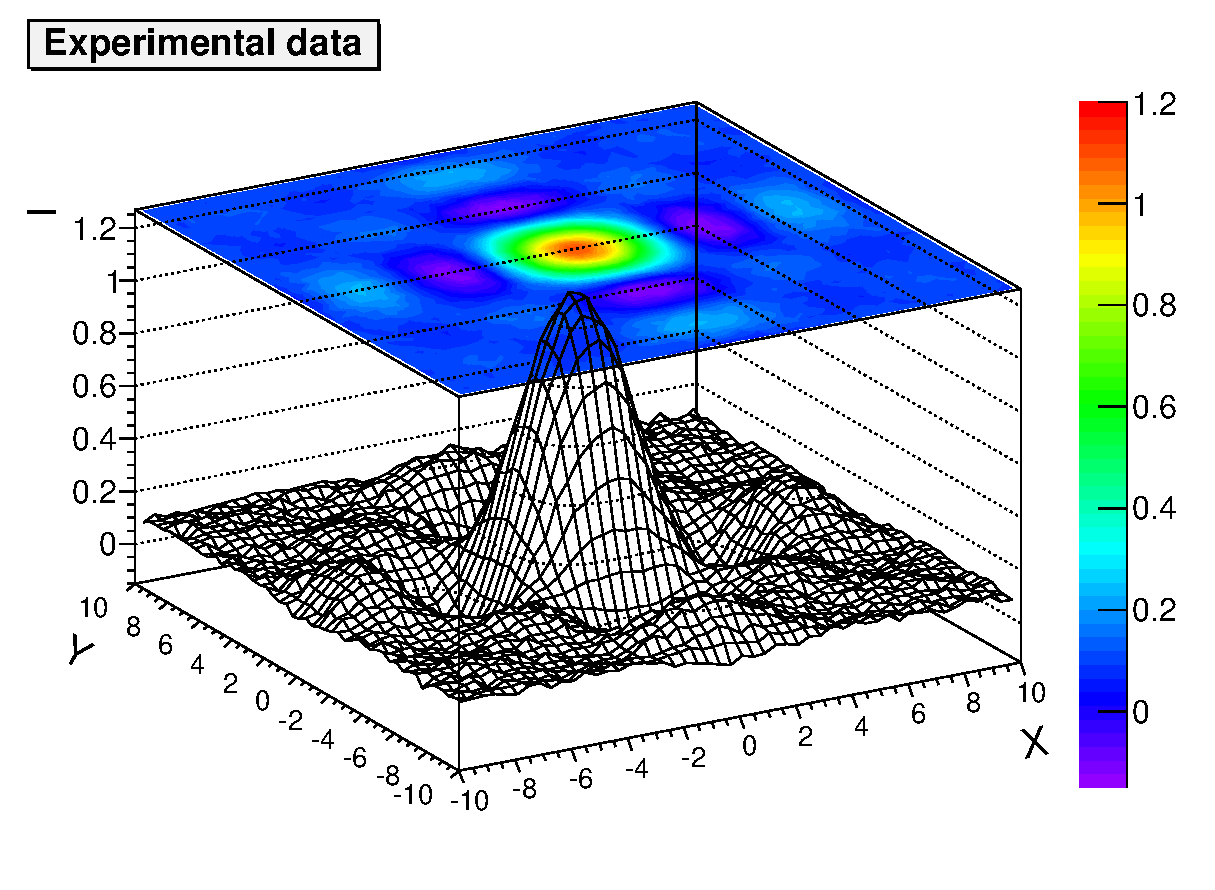
\includegraphics[width=0.49\textwidth]{Figures/toyfit_expdata.eps}
    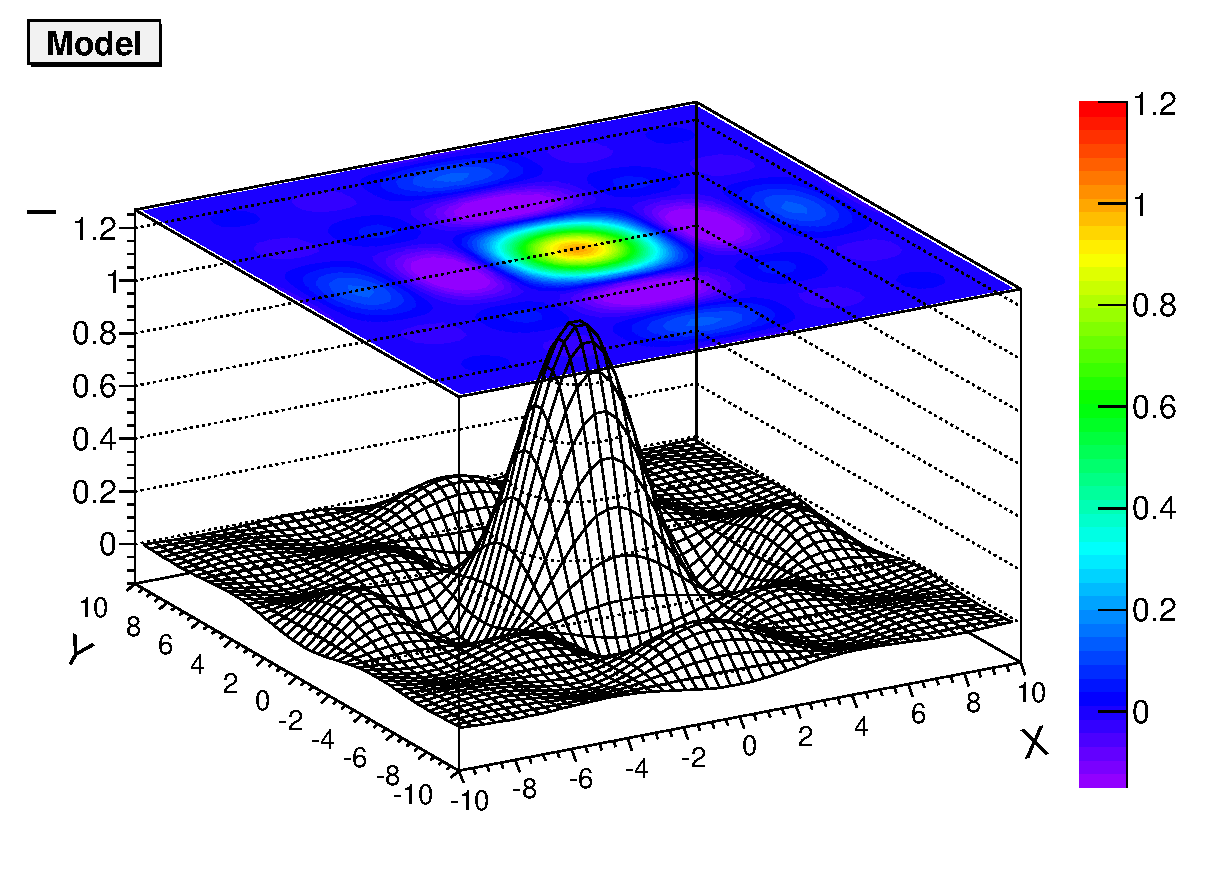
\includegraphics[width=0.49\textwidth]{Figures/toyfit_simdata.eps}
  \caption{Intensity as a function of (x,y) detector coordinates  obtained from 
  toy experiment (left) and from the toy simulation (right).   }
  \label{fig:toyfit_data}
  \vspace*{4mm}
    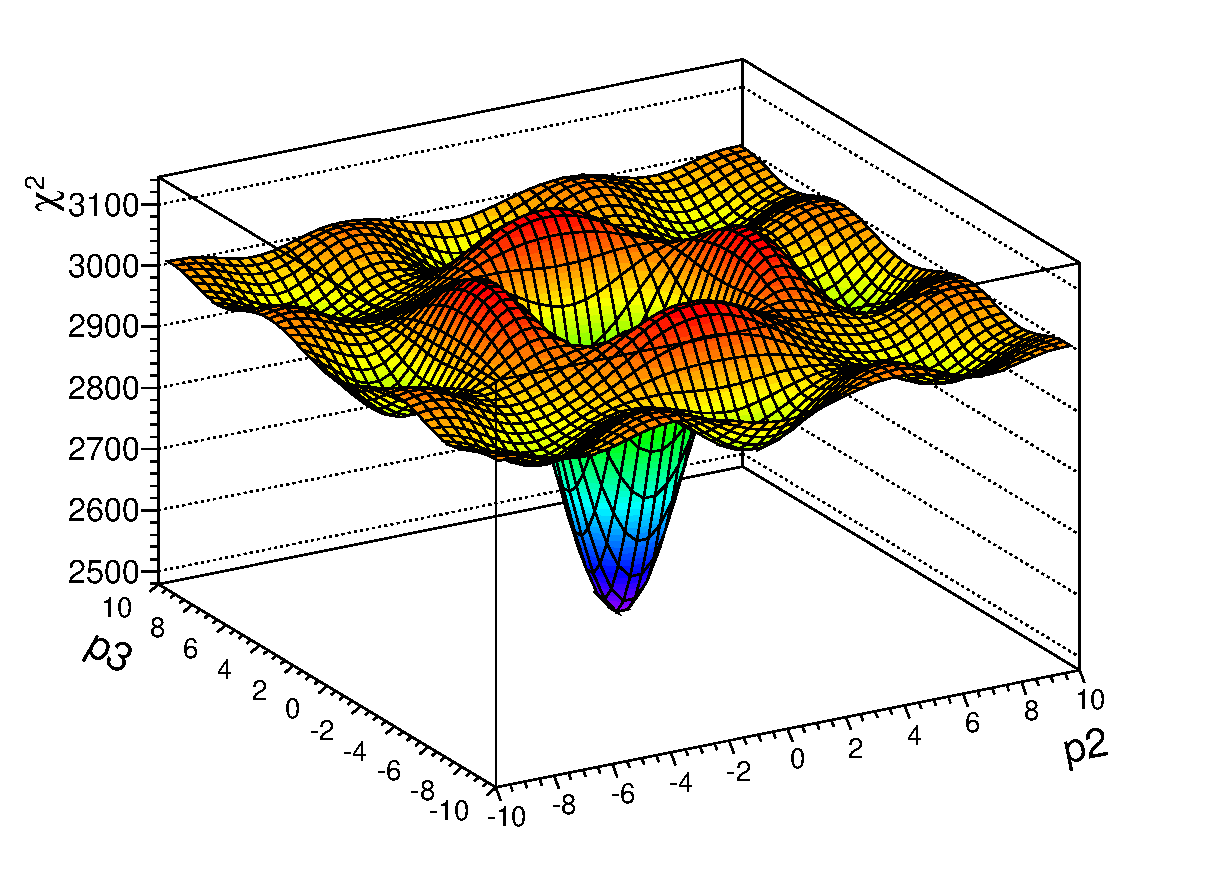
\includegraphics[width=0.49\textwidth]{Figures/toyfit_chi2_p23.eps}
    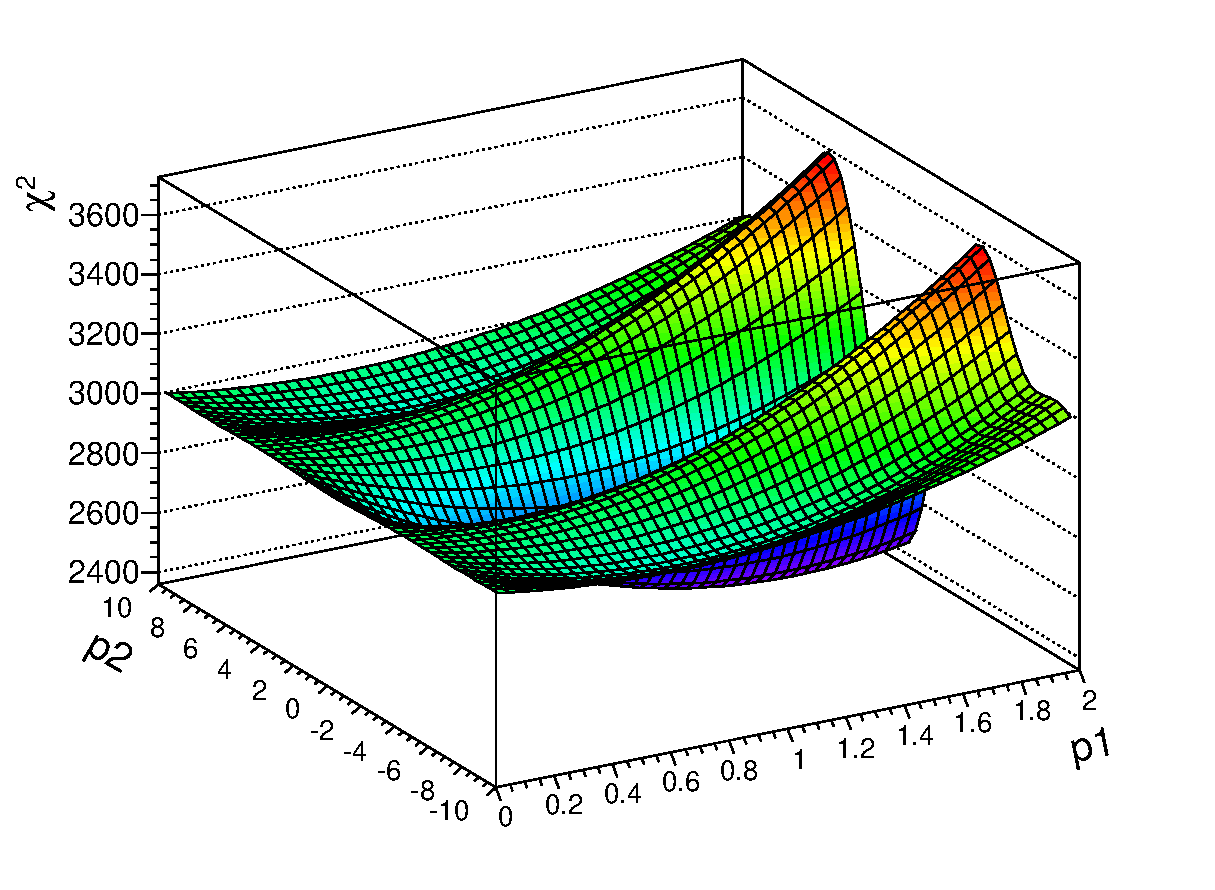
\includegraphics[width=0.49\textwidth]{Figures/toyfit_chi2_p12.eps}
  \caption{$\chi^{2}$ value calculated between experimental and simulated data
  as a function of $p_2,p_3$ parameters (left) or $p_1,p_2$ 
  parameters (right) used in the model.   }
  \label{fig:toyfit_chi2}
\end{figure}


Scattering picture presented reminds some of GISAS patterns, nevertheless it is
generated using simple function
$$I(x,y) = G(0.1,~0.01) + \frac{sin(x)}{x} \cdot \frac{sin(y)}{y}$$
Here $G(0.1, 0.01)$ is a random variable distributed according to the Gaussian distribution
with mean 0.1 and $\sigma=0.01$.
Constant $0.1$ symbolize our experimental background and constant $0.01$ is referred
to the detector noise. The rest of the formula represents our signal.

Lets define our model, namely specific mathematical function, to which we will fit our toy experimental data. By making an educated guess we assume that scattering intensity observed
in the experiment should be described with the help of $sinc$ function as follows
$$ f(x,y) = p_0 + p_1 \cdot  sinc(x - p_2) \cdot sinc(y - p_3) $$
The model has four parameters: $p_0$ describing background, $p_{1}$ describing signal strength
and $p_2,p_3$ responsible for the peak position.
Fig.~\ref{fig:toyfit_data},right shows the intensity as a function (x,y) calculated according
our model using fixed parameter set $p_0=0,p_1=1,p_2=0,p_3=0$. 

Two distributions look pretty much the same, however to find exact values of parameters which describe experimental data in the best way, one have to
\begin{itemize}
\item elaborate criteria for the difference between an actual data and its model
\item employ minimization procedure which will minimize that difference
\end{itemize}


\subsection{Objectives}

The goal is to obtain the best fit of an observed distribution
to a prediction by modifying a set of parameters from the
prediction. This problem can be one or multi-dimensional and also linear or
nonlinear. The quantity to minimize is often referred to as the
\textit{objective function}, whose expression depends on the
particular method, like the maximum likelihood, the $\chi^2$
minimization or the expected prediction error function. 

\begin{comment}
\subsubsection*{Maximum of likelihood.}
This is a popular method for parameters' estimations because the maximum likelihood estimators are approximately
unbiased and efficient for large data samples, under quite general
conditions.
We assume a sample  $\mathbf{x}=\{x_{1},x_{2},...,x_{n}\}$ of n independent and identically distributed
observations coming from probability density function $f(\mathbf{x}; \mathbf{p})$.
We assume $f(\mathbf{x}; \mathbf{p})$
to be known except for the parameters $\mathbf{p}=\{p_1,p_2,...,p_3\}$
The method of maximum likelihood takes the estimators to be
those values of $\mathbf{p}$ that maximize the likelihood function $\mathcal{L}$ as
$\mathcal{L}(\mathbf{\alpha})=\prod_{i=1}^N f(x_i;\mathbf{p})$.
Since it is easier to deal with a sum, we usually minimize
$-\text{ln}(\mathcal{L})$.
\end{comment}


\subsubsection*{$\chi^2$ or least squares minimization}
A dataset consist of $n$ data pairs $(\mathbf{x_{i}}, a_{i}), i=1,N$ where 
$\mathbf{x_{i}}$ is an independent variable and $a_{i}$ is dependent variable, whose
value is found in the measurement $i$. The number $N$ denotes the total
number of measurements. 

In the case of intensity map measured in our toy experiment 
and presented in Fig~\ref{fig:toyfit_data}, a variable $a_{i}$ denotes measured intensity, a variable $\mathbf{x_{i}}$ is a vector and correspond to the 
$(x_{i}, y_{i})$ coordinates of pixels in our detector while number $N$  corresponds 
to total number of detector pixels.

The model function has the form
$f(\mathbf{x_{i}},\mathbf{p})$
where adjustable parameters are held in the vector $\mathbf{p}$.
The least squared method finds the optimum of model function which 
fit the data in the best way by searching for the minimum of the sum of squared
residuals
$$ \chi^{2}(\mathbf{p}) = \sum_{i=1}^{N}r_{i}^{2}$$
where residual is defined as the difference between measured value and the value predicted by the model.
$$r = a_{i} - f(\mathbf{x_{i}},\mathbf{p})$$

In the case of normally distributed variables with the $\sigma^2$ variance
the quantity to minimize becomes
$$ \chi^{2}(\mathbf{p}) =
\frac{1}{d}
\sum_{i=1}^{N}  
\frac{ (a_{i} - f(\mathbf{x_{i}},\mathbf{p}))^2}{\sigma^2}   $$
where $d=N-k$ is number of degree of freedom ($k$ number of free fit parameters).


\subsubsection*{Minimization algorithms}
There are a large number of minimization algorithms providing a solution to the problem
of minimizing the objective function over the space of parameters of the function.
The minimization starts from initial guess for the parameters provided by the user,
and then evolves iteratively under control of minimization algorithm. The procedural
modifications on the parameters, the objective function, as well as convergence
criterion depend on the method implemented.
Details of particular implementation is beyond the scope of this manual and
 interested reader is encouraged to look at outside resources.



\subsubsection*{Local minima trap}




\subsection{Terminology.}

\noindent
{\bf Reference data} \\
Normally just experimental data or might be also simulated data
spoiled with the noise for purpose of testing of minimization algorithms.
\vspace*{1mm}

\noindent
{\bf Objective function} \\
Subject of minimization procedure.
\vspace*{1mm}

\noindent
{\bf Minimization} \\
Finding a best available values (i.e. local minimum) of some objective function. 
\vspace*{1mm}

\noindent
{\bf Number of degrees of freedom} \\
Number of data points - number of parameters in the fit.
\vspace*{1mm}

\noindent
{\bf Minimizer} \\
An algorithm which minimize objective function. 



%%%%%%%%%%%%%%%%%%%%%%%%%%%%%%%%%%%%%%%%%%%%%%%%%%%%%%%%%%%%%%%%%%%%%%%%%%%%%%%
%
%%%%%%%%%%%%%%%%%%%%%%%%%%%%%%%%%%%%%%%%%%%%%%%%%%%%%%%%%%%%%%%%%%%%%%%%%%%%%%%
\section{Implementation in BornAgain} \SecLabel{FittingImplementation}

Fitting in  \BornAgain\ deals with estimating the optimum parameters
in the numerical model by minimizing the difference between
numerical and reference data.
%using $\chi^2$  or maximum likelihood methods. 
The features include 

\begin{itemize}
\item a variety of multidimensional minimization algorithms and strategies.
\item the choice over possible fitting parameters, their properties and correlations.
\item the full control on objective function calculations, including applications of different normalizations and assignments of different masks and weights to different areas of reference data.
\item the possibility to fit simultaneously an arbitrary number of data sets.
\end{itemize}

Figure ~\ref{fig:minimization_workflow} shows general work flow of a typical fitting procedure.
\begin{figure}[htbp]
\centering
  \resizebox{0.99\textwidth}{!}{%
    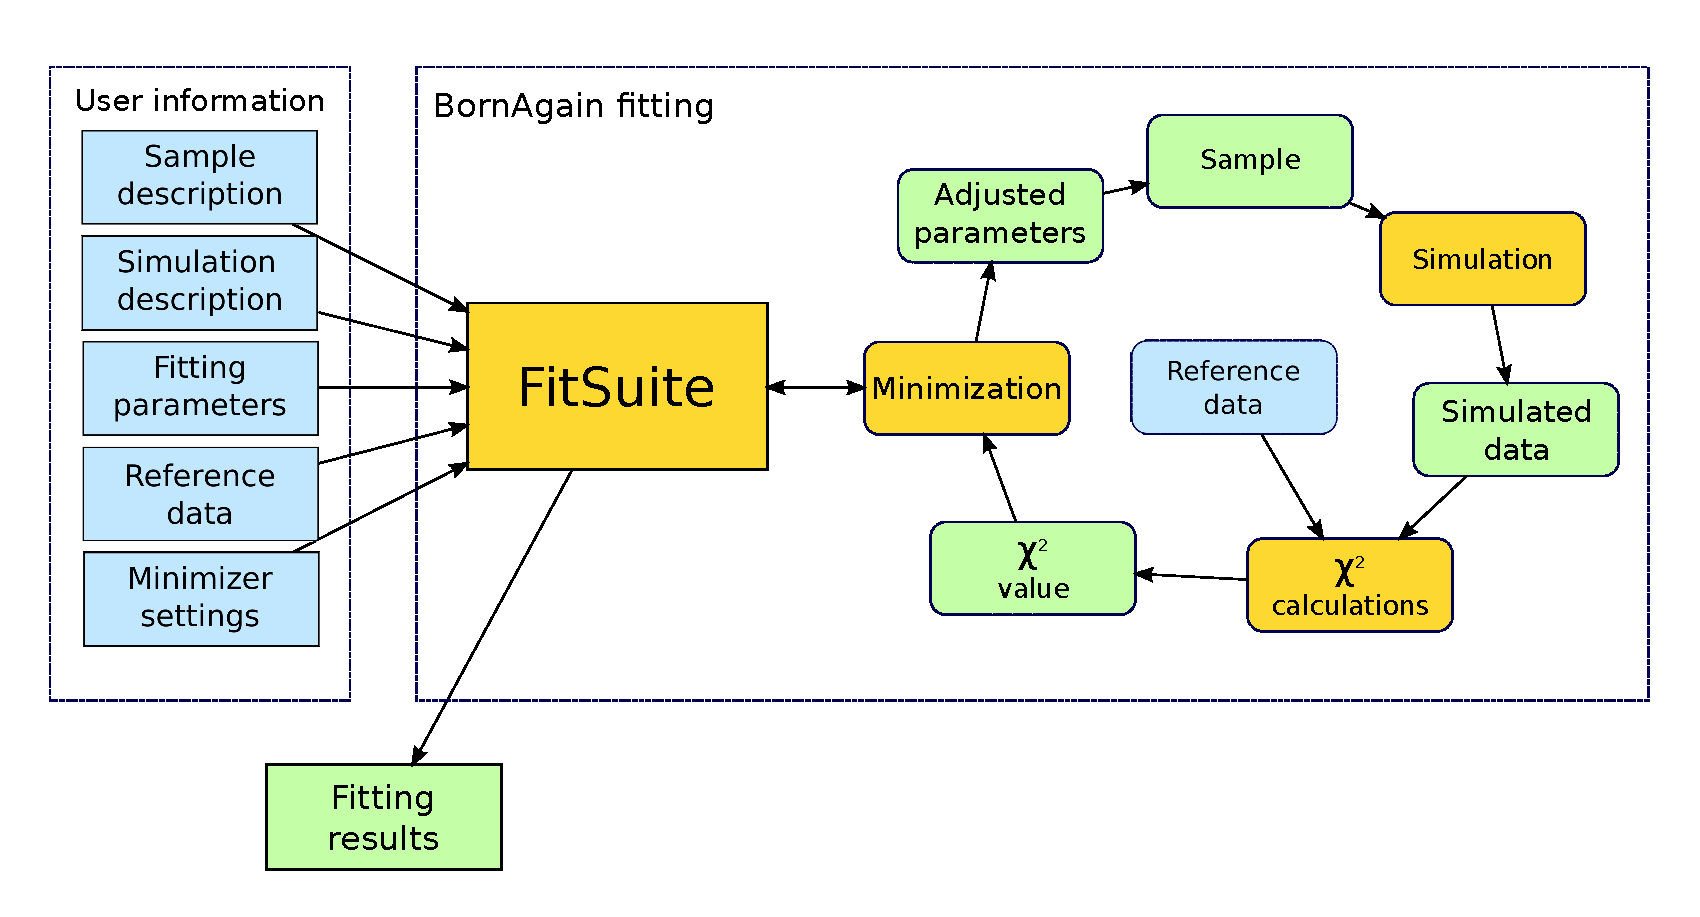
\includegraphics{Figures/minimization_workflow.eps}}
\caption{
Fitting work flow.
}
\label{fig:minimization_workflow}
\end{figure}

Before running the fitting the user is required to prepare some  data and to
configure the fitting kernel of \BornAgain\ . The required stages are

\begin{itemize}
\item Preparing the sample and the simulation description (multilayer, beam, detector parameters).
\item Choosing the fitting parameters.
\item Loading the reference data.
\item Defining the minimization settings.
\end{itemize}

The class \Code{FitSuite} contains the main functionalities to be used for the fit
and serves as the main interface between the user and the fitting work flow. 
The later involves iterations during which

\begin{itemize}
\item The minimizer makes an assumption about the optimal sample parameters.
\item These parameters are propagated to the sample.
\item The simulation is performed for the given state of the sample.
\item The simulated data (intensities) are propagated to the $\chi^2$ module.
\item The later calculates $\chi^2$ using the simulated and reference data.
\item The value of $\chi^2$ is propagated to the minimizer, which makes new assumptions about optimal sample parameters.
\end{itemize}

The iteration process is going on under the control of the selected minimization
algorithm, without any intervention from the
user. It stops 
\begin{itemize}
\item when the maximum number of iteration steps has been exceeded,
\item when the function's minimum has been reached within the tolerance window,
\item if the minimizer could not improve the values of the parameters. 
\end{itemize}

After the control is returned, fitting results can be retrieved.
They consist in the best $\chi^2$ value found, the corresponding
optimal sample parameters and the intensity map simulated with this set of parameters.

Details of \Code{FitSuite} class implementation and description
of each interface are given in \SecRef{FitSuiteClass}. The following parts of this section will detail each of
the main stages necessary to run a fitting procedure.


%%%%%%%%%%%%%%%%%%%%%%%%%%%%%%%%%%%%%%%%%%%%%%%%%%%%%%%%%%%%%%%%%%%%%%%%%%%%%%%
%
%%%%%%%%%%%%%%%%%%%%%%%%%%%%%%%%%%%%%%%%%%%%%%%%%%%%%%%%%%%%%%%%%%%%%%%%%%%%%%%
\subsection{Preparing the sample and the simulation description}

This step is similar for any simulation using \BornAgain\ (see \SecRef{Simulation}). It consists in first characterizing  the geometry of the system: the particles 
(shapes, sizes, refractive
indices), the different layers (thickness,
order, refractive index, a possible roughness of the interface), the
interference between the particles and the way they are distributed in
the layers (buried particles or particles sitting on top of a
layer). 
Then we specify the parameters of the input beam and of the
output detector.


%%%%%%%%%%%%%%%%%%%%%%%%%%%%%%%%%%%%%%%%%%%%%%%%%%%%%%%%%%%%%%%%%%%%%%%%%%%%%%%
%
%%%%%%%%%%%%%%%%%%%%%%%%%%%%%%%%%%%%%%%%%%%%%%%%%%%%%%%%%%%%%%%%%%%%%%%%%%%%%%%
\subsection{Choice of parameters to be fitted}
In principle, every parameter used in the construction of the sample
can be used as a fitting parameter. For example, the particles'
heights, radii or the layer's roughness or thickness could be selected
using the 
parameter pool mechanism. 
This mechanism is explained in detail in
\SecRef{WorkingWithSampleParameters} and it is therefore recommended
to read it before proceeding any further.

The user specifies selected sample parameters as fit parameters using \Code{FitSuite}
and its \Code{addFitParameter} method
\begin{lstlisting}[language=shell, style=commandline]
fit_suite = FitSuite()
fit_suite.addFitParameter(<name>, <initial value>, <step>, <limits>)
\end{lstlisting}
where \Code{<name>} corresponds to the parameter name in the sample's parameter pool.
By using wildcards in the parameter name, a group of sample parameters, corresponding to the given
pattern, can be associated with a single fitting parameter and 
fitted simultaneously to get a common optimal value (see \SecRef{WorkingWithSampleParameters}).

The second parameter \Code <initial value> correspond to the initial value of
the fitting parameter, while the third one
is responsible to the initial iteration steps size.
The last parameter \Code{<AttLimits>} corresponds to
the boundaries imposed on parameter value. It can be
\begin{itemize}
\item \Code{limitless()} by default, 
\item \Code{fixed()}, 
\item \Code{lowerLimited(<min\_value>)}, 
\item \Code{upperLimited(<max\_value>)}, 
\item \Code{limited(<min\_value>, <max\_value>)}.
\end{itemize}
where \Code{<min\_value>} and \Code{<max\_value>} are
double values corresponding to the lower and higher boundary, respectively.


%%%%%%%%%%%%%%%%%%%%%%%%%%%%%%%%%%%%%%%%%%%%%%%%%%%%%%%%%%%%%%%%%%%%%%%%%%%%%%%
%
%%%%%%%%%%%%%%%%%%%%%%%%%%%%%%%%%%%%%%%%%%%%%%%%%%%%%%%%%%%%%%%%%%%%%%%%%%%%%%%
\subsection{Associating reference and simulated data}

The minimization procedure deals with a pair of reference data (normally
associated with experimental data) and the theoretical model (presented by the sample and the simulation descriptions).

We assume that the experimental data are a two-dimensional intensity 
matrix as function of the output scattering
angles $\alpha_f$ and $\phi_f$ (see Fig.~\ref{fig:multil3d}).
The user is required to provide the data in the form of an ASCII file
containing an axes
binning description and the intensity data itself. 
\vspace*{2mm}

\ImportantPoint{Remark:}{
We recognize the importance of supporting the most common data formats. We are going to provide
this feature in the following releases and welcome users' requests on this subject.
}
\vspace*{1mm}

To associate the simulation and the reference data to the fitting engine, method \newline
\Code{addSimulationAndRealData} has to be used as shown
\begin{lstlisting}[language=python, style=eclipseboxed,numbers=none]
fit_suite = FitSuite()
fit_suite.addSimulationAndRealData(<simulation>, <reference>, <chi2_module>)
\end{lstlisting}

Here \Code{<simulation>} corresponds to a \BornAgain\ simulation object
with the  sample, beam and detector fully defined, \Code{<reference>}
corresponds to the experimental data object obtained from the ASCII file and \Code{<chi2\_module>} is an optional parameter for advanced 
control of $\chi2$ calculations.

It is possible to call this given method more than once to submit more than one pair of
\Code{<simulation>, <reference>} to the fitting procedure.
In this way, simultaneous fits of
some combined data sets are performed.

By using the third \Code{<chi2\_module>} parameter, different normalizations and weights
can be applied to give user full control of the way $\chi2$ is calculated.
This feature will be explained in \SecRef{FittingAdvanced}.


%%%%%%%%%%%%%%%%%%%%%%%%%%%%%%%%%%%%%%%%%%%%%%%%%%%%%%%%%%%%%%%%%%%%%%%%%%%%%%%
%
%%%%%%%%%%%%%%%%%%%%%%%%%%%%%%%%%%%%%%%%%%%%%%%%%%%%%%%%%%%%%%%%%%%%%%%%%%%%%%%
\subsection{Minimizer settings}

\BornAgain\ contains a variety of minimization engines from \Code{ROOT} and \Code{GSL}
libraries. They are listed in Table~\ref{table:fit_minimizers}.
By default \Code{Minuit2} minimizer with default settings will be used and no additional
configuration needs to be done.
The remainder of this section explains some of the expert settings, which can be applied to get better 
fit results.

The default minimization algorithm can be changed using 
\Code{MinimizerFactory} as shown below
\begin{lstlisting}[language=python, style=eclipseboxed,numbers=none]
fit_suite = FitSuite()
minimizer = MinimizerFactory.createMinimizer("<Minimizer name>","<algorithm>")
fit_suite.setMinimizer(minimizer)
\end{lstlisting}

where \Code{<Minimizer name>} and \Code{<algorithm>} can be chosen from the first and
second column of Table~\ref{table:fit_minimizers} respectively. 
The list of minimization algorithms implemented in \BornAgain\
can also be obtained using \Code{MinimizerFactory.printCatalogue()} command.


\begin{table}[h]
\centering
\begin{tabular}{@{}lll@{}}
\hline
\hline
\textbf{Minimizer name} & \textbf{Algorithm} & \textbf{Description}\\
\hline
\Code{Minuit2} \cite{MinuitURL} & \Code{Migrad} & According to
\cite{mntutorial} best minimizer for nearly all functions,\\
 & & variable-metric method with inexact line search, \\
 & & a stable metric updating scheme,\\
 & &  and checks for positive-definiteness.\\
\hline
                                       & \Code{Simplex} & simplex method of
                                       Nelder and Mead\\ 
 & & usually slower than \Code{Migrad}, \\
 &  & rather robust with respect to gross fluctuations in the\\ & &  function
 value, gives no reliable information about \\ & &  parameter errors, \\
\hline
                                       & \Code{Combined} & minimization with
                                       \Code{Migrad} \\
                                       & & but switches to Simplex if
                                       Migrad fails to converge.\\
\hline
                                       & \Code{Scan} &  not intended to
                                       minimize, just scans the
                                       function,\\
                                       & &  one parameter at a
                                       time, retains the best value
                                       after\\ &  & each scan\\
\hline
                                       & \Code{Fumili} & optimized
                                       method for least square and log
                                       likelihood\\ & &  minimizations \\
\hline
\Code{GSLMultiMin} \cite{GSLMultiMinURL} & \Code{ConjugateFR} & Fletcher-Reeves conjugate gradient
  algorithm,\\
\hline
& \Code{ConjugatePR} & Polak-Ribiere conjugate gradient algorithm,\\ 
\hline
& \Code{BFGS} & Broyden-Fletcher-Goldfarb-Shanno algorithm,\\ 
\hline
& \Code{BFGS2} & improved version of BFGS,\\ 
\hline
& \Code{SteepestDescent} & follows the downhill gradient of the function at each step\\
\hline
\Code{GSLMultiFit} \cite{GSLMultiFitURL} & & Levenberg-Marquardt
Algorithm\\
\hline
\Code{GSLSimAn} \cite{GSLSimAnURL}& & Simulated Annealing Algorithm\\ 
\hline
\hline
\end{tabular}
\caption{List of minimizers implemented in \BornAgain. }
\label{table:fit_minimizers}
\end{table}

There are several options common to every minimization algorithm, which can be changed
before starting the minimization. They are handled by \Code{MinimizerOptions} class:
\begin{lstlisting}[language=python, style=eclipseboxed, numbers = none]
options = MinimizerOptions()
options.setMaxFunctionCalls(10)
fit_suite.getMinimizer().setOptions(options)
\end{lstlisting}
In the above code snippet, a number of ``maximum function calls'',
namely the maximum number of times the minimizer is allowed to call the simulation, is limited to 10. %The minimizer will take that number into consideration and will try to limit number of iterations by that value.

There are also expert-level options common for all minimizers as well
as a number of options to tune individual minimization algorithms.
They will be explained in \SecRef{FittingAdvanced}.


%%%%%%%%%%%%%%%%%%%%%%%%%%%%%%%%%%%%%%%%%%%%%%%%%%%%%%%%%%%%%%%%%%%%%%%%%%%%%%%
%
%%%%%%%%%%%%%%%%%%%%%%%%%%%%%%%%%%%%%%%%%%%%%%%%%%%%%%%%%%%%%%%%%%%%%%%%%%%%%%%
\subsection{Running the fitting ant retrieving the results}

After the initial configuration of \Code{FitSuite} has been performed, the fitting
can be started using the command
\begin{lstlisting}[language=python, style=eclipseboxed, numbers = none]
fit_suite.runFit()
\end{lstlisting}

Depending on the complexity of the sample and the number of free sample parameters the fitting
process can take from tens to thousands of iterations. The results of the fit can
be printed on the screen using the command
\begin{lstlisting}[language=python, style=eclipseboxed, numbers = none]
fit_suite.printResults()
\end{lstlisting}
\SecRef{FittingExamples} gives more details about how to access the fitting results.




\section{Basic Python fitting example} \SecLabel{FittingExamples}

In this section we are going to go through a complete example of
fitting using \BornAgain. Each  step will be associated with a
detailed piece of code written in \Python. 
The complete listing of
the script is given in Appendix (see Listing~\ref{PythonFittingExampleScript}).
The script can also be found at
\begin{lstlisting}[language=shell, style=commandline]
./Examples/python/fitting/ex002_FitCylindersAndPrisms/FitCylindersAndPrisms.py
\end{lstlisting}

\noindent
This example uses the same sample geometry as in \SecRef{Example1Python}.
Cylindrical and
prismatic particles in equal proportion are deposited on a substrate layer, with no interference
between the particles. We consider the following parameters to be unkown
\begin{itemize}
\item the radius of cylinders,
\item the height of cylinders,
\item the length of the prisms' triangular basis,
\item the height of prisms.
\end{itemize}

Our reference data are a ``noisy'' two-dimensional intensity
map obtained from the simulation of the same geometry with a fixed
value of $5\,{\rm nm}$ for the height and radius of cylinders and for the
height of prisms which have a 10-nanometer-long side length. 
Then we run our fitting using default minimizer settings
starting with a cylinder's height
of $4\,{\rm nm}$, a cylinder's radius of $6\,{\rm nm}$, 
a prism's half side of $6\,{\rm nm}$ and a height equal to $4\,{\rm nm}$.
As a result, the fitting procedure is able to find the correct value of $5\,{\rm nm}$
for all four parameters.


%%%%%%%%%%%%%%%%%%%%%%%%%%%%%%%%%%%%%%%%%%%%%%%%%%%%%%%%%%%%%%%%%%%%%%%%%%%%%%%
\subsubsection*{Importing Python libraries}
\begin{lstlisting}[language=python, style=eclipseboxed]
from libBornAgainCore import *
from libBornAgainFit import *
\end{lstlisting}
We start from importing two \BornAgain\ libraries required to create
the sample description
and to run the fitting.


%%%%%%%%%%%%%%%%%%%%%%%%%%%%%%%%%%%%%%%%%%%%%%%%%%%%%%%%%%%%%%%%%%%%%%%%%%%%%%%
\subsubsection*{Building the sample}
\begin{lstlisting}[language=python, style=eclipseboxed, firstnumber=5]
def get_sample(): @\label{script2::get_sample}@
    """
    Build the sample representing cylinders and pyramids on top of substrate without interference.
    """
    # defining materials
    m_air = HomogeneousMaterial("Air", 0.0, 0.0)
    m_substrate = HomogeneousMaterial("Substrate", 6e-6, 2e-8)
    m_particle = HomogeneousMaterial("Particle", 6e-4, 2e-8)

    # collection of particles
    cylinder_ff = FormFactorCylinder(1.0*nanometer, 1.0*nanometer)
    cylinder = Particle(m_particle, cylinder_ff)
    prism_ff = FormFactorPrism3(2.0*nanometer, 1.0*nanometer)
    prism = Particle(m_particle, prism_ff)
    particle_layout = ParticleLayout()
    particle_layout.addParticle(cylinder, 0.0, 0.5)
    particle_layout.addParticle(prism, 0.0, 0.5)
    interference = InterferenceFunctionNone()
    particle_layout.addInterferenceFunction(interference)

    # air layer with particles and substrate form multi layer
    air_layer = Layer(m_air)
    air_layer.setLayout(particle_layout)
    substrate_layer = Layer(m_substrate)
    multi_layer = MultiLayer()
    multi_layer.addLayer(air_layer)
    multi_layer.addLayer(substrate_layer)
    return multi_layer
\end{lstlisting}
The function starting at line~\ref{script2::get_sample} creates a multilayered sample
with cylinders and prisms using arbitrary $1\,{\rm nm}$ value for all size's of particles.
The details about the generation of this multilayered sample are given in \SecRef{Example1Python}.


%%%%%%%%%%%%%%%%%%%%%%%%%%%%%%%%%%%%%%%%%%%%%%%%%%%%%%%%%%%%%%%%%%%%%%%%%%%%%%%
\subsubsection*{Creating the simulation}
\begin{lstlisting}[language=python, style=eclipseboxed, firstnumber=35]
def get_simulation(): @\label{script2::get_simulation}@
    """
    Create GISAXS simulation with beam and detector defined
    """
    simulation = Simulation()
    simulation.setDetectorParameters(100, -1.0*degree, 1.0*degree, 100, 0.0*degree, 2.0*degree)
    simulation.setBeamParameters(1.0*angstrom, 0.2*degree, 0.0*degree)
    return simulation
\end{lstlisting}
The function starting at line~\ref{script2::get_simulation} creates
the simulation object with the definition of the beam and detector parameters.



%%%%%%%%%%%%%%%%%%%%%%%%%%%%%%%%%%%%%%%%%%%%%%%%%%%%%%%%%%%%%%%%%%%%%%%%%%%%%%%
\subsubsection*{Preparing the fitting pair}
\begin{lstlisting}[language=python, style=eclipseboxed, firstnumber=45]
def run_fitting(): @\label{script2::run_fitting}@
    """
    run fitting
    """
    sample = get_sample() @\label{script2::setup_simulation1}@
    simulation = get_simulation()
    simulation.setSample(sample) @\label{script2::setup_simulation2}@

    real_data = IntensityDataIOFactory.readIntensityData('refdata_fitcylinderprisms.txt') @\label{script2::real_data}@
\end{lstlisting}
Lines
~\ref{script2::setup_simulation1}-~\ref{script2::setup_simulation2}
generate the 
sample and simulation description and assign the sample to the simulation.
Our reference data are contained in the file \Code{'refdata\_fitcylinderprisms.txt'}.
 This reference had been generated by adding noise
on the scattered intensity from a numerical sample with a fixed length of 5~nm for the four fitting
parameters (\textit{i.e.} the dimensions of the cylinders and prisms).
Line ~\ref{script2::real_data} creates the real data object by loading
the ASCII data from the input file.


%%%%%%%%%%%%%%%%%%%%%%%%%%%%%%%%%%%%%%%%%%%%%%%%%%%%%%%%%%%%%%%%%%%%%%%%%%%%%%%
\subsubsection*{Setting up \rm\bf{FitSuite}}
\begin{lstlisting}[language=python, style=eclipseboxed, firstnumber=55]
    fit_suite = FitSuite() @\label{script2::fitsuite1}@
    fit_suite.addSimulationAndRealData(simulation, real_data) @\label{script2::fitsuite2}@
    fit_suite.initPrint(10) @\label{script2::fitsuite3}@
\end{lstlisting}
Line ~\ref{script2::fitsuite1} creates a \Code{FitSuite} object which provides
the main interface to the minimization kernel of \BornAgain\ . 
Line ~\ref{script2::fitsuite2} submits simulation description and real data pair to the 
subsequent fitting. Line ~\ref{script2::fitsuite3} sets up \Code{FitSuite} to print on
the screen the information about fit progress once per 10 iterations.
\begin{lstlisting}[language=python, style=eclipseboxed, firstnumber=60]
    fit_suite.addFitParameter("*FormFactorCylinder/height", 4.*nanometer, 0.01*nanometer, AttLimits.lowerLimited(0.01)) @\label{script2::fitpars1}@
    fit_suite.addFitParameter("*FormFactorCylinder/radius", 6.*nanometer, 0.01*nanometer, AttLimits.lowerLimited(0.01))
    fit_suite.addFitParameter("*FormFactorPrism3/height", 4.*nanometer, 0.01*nanometer, AttLimits.lowerLimited(0.01))
    fit_suite.addFitParameter("*FormFactorPrism3/length", 12.*nanometer, 0.02*nanometer, AttLimits.lowerLimited(0.01)) @\label{script2::fitpars2}@
\end{lstlisting}
Lines ~\ref{script2::fitpars1}--~\ref{script2::fitpars2} enter the
list of fitting parameters. Here we use the cylinders' height and
radius and the prisms' height and side length. 
The cylinder's length and prism half side are initially equal to $4\,{\rm nm}$,
whereas the cylinder's radius and the prism half side length are equal to $6\,{\rm nm}$ before the minimization. The
iteration step is equal to $0.01\,{\rm nm}$ and only the lower
boundary is imposed to be equal to $0.01\,{\rm nm}$.


%%%%%%%%%%%%%%%%%%%%%%%%%%%%%%%%%%%%%%%%%%%%%%%%%%%%%%%%%%%%%%%%%%%%%%%%%%%%%%%
\subsubsection*{Running the fit and accessing results}
\begin{lstlisting}[language=python, style=eclipseboxed, firstnumber=66]
    fit_suite.runFit() @\label{script2::fitresults1}@

    print "Fitting completed."
    fit_suite.printResults()@\label{script2::fitresults2}@
    print "chi2:", fit_suite.getMinimizer().getMinValue() 
    fitpars = fit_suite.getFitParameters()
    for i in range(0, fitpars.size()):
        print fitpars[i].getName(), fitpars[i].getValue(), fitpars[i].getError() @\label{script2::fitresults3}@
\end{lstlisting}
Line ~\ref{script2::fitresults1} shows the command to start the fitting process.
During the fitting the progress will be displayed on the screen.
Lines ~\ref{script2::fitresults2}--~\ref{script2::fitresults3} shows different ways of
accessing the fit results.


More details about fitting, access to its results and visualization of
the fit progress using matplotlib libraries can be learned from the
following detailed example
\begin{lstlisting}[language=shell, style=commandline]
./Examples/python/fitting/ex002_FitCylindersAndPrisms/FitCylindersAndPrisms_detailed.py
\end{lstlisting}



\section {Advanced fitting.} \SecLabel{FittingAdvanced}

\subsection{Affecting $\chi2$ calculations.}
\subsection{Simultaneous fit of several data sets.}
\subsection{Using fitting strategies.}
\subsection{Masking the real data.}
\subsection{Tuning fitting algorithms.}
\subsection{Fitting with correlated sample parameters.}



\section {How to get right answer from fitting.} 
\SecLabel{FittingRightAnswers}

As it was already mentioned in \SecRef{FittingGentleIntroducion}, 
one of the main difficulties in fitting the data with the model 
is the presence of multiple
local minima in the objective function. The extended list of problems causing fit to failure includes
\begin{itemize}
\item unreliable physical model
\item multiple local minima
\item unphysical behavior of objective function, unphysical regions in parameter space
\item unreliable parameter error calculation in the presence of limits on parameter value
\item often exponential behavior of objective function and corresponding numerical inaccuracies and excessive numerical roundoff in calculation of its value and derivatives
\item large correlations between parameters
\item very different scale of parameters involved in calculation
\item not positive definite error matrix even at minimum
\end{itemize}


Given list, of course, is unrelated only to \BornAgain\ fitting. It remains the same
while fitting the data with any fitting program and any kind of theoretical model.
To address all these difficulties some amount of manual tuning might be necessary. Below we give some recommendations which might help the user to achieve reliable fit results.

\subsection*{General recommendation}
\begin{itemize}
\item initially choose small number of free fitting parameters
\item eliminate redundand parameters
\item provide a good initial guess for fit parameters
\item start from default minimizer settings and turn to the fine tuning after some experience has been acquired.
\item repeat fit using different starting values for parameters or their limits
\item repeat fit fixing and releasing different groups  of parameters
\item use \Code{Minuit2} minimizer with \Code{Migrad} algorithm (default) to get most reliable parameter error estimation
\item try \Code{GSLMultiFit} minimizer or \Code{Minuit2} minimizer with \Code{Fumili} algorithm to get fewer iterations


%\subsection*{Interpretation of errors.}


{\bf to be continued... }


\end{itemize}





%\newpage
\chapter{Software architecture}\SecLabel{SoftwareArchitecture}
 

\BornAgain\ is written on C++
and uses object oriented approach to 
achieve modularity, extensibility and transparency.
This leads to the task driven rather then command driven approach in 
different aspects  of the simulation and fitting of GISAS data.
User defines the sample structure, beam and detector characteristics,
fit parameters, using building
blocks -- \Code{classes} -- defined in kernel libraries of the framework.
These buildings blocks are combined together by the user according to his current
task using one the following approach.
\begin{itemize}
\item User imports \BornAgain\ libraries into the python to extent it
with \BornAgain\ API and then prepare python script with sample description and simulation settings. 
User runs the simulation by executing script in python interpreter and then assess
simulation results using the way he likes, e.g. python + numpy + matplotlib.
\item User may construct standalone C++ application linked to \BornAgain\ libraries.
\item User interacts with the framework through graphical 
user drag-and-drop interface (forthcoming).
\end{itemize}

Object oriented approach in the simulation design allows 
to reach much higher level of flexibility in sample construction, 
decouple interdependence in internal calculations and so facilitate creation of new models
that entails little or no modification to the existing code. 


\begin{figure}[htbp]
\centering
  \resizebox{0.9\textwidth}{!}{%
    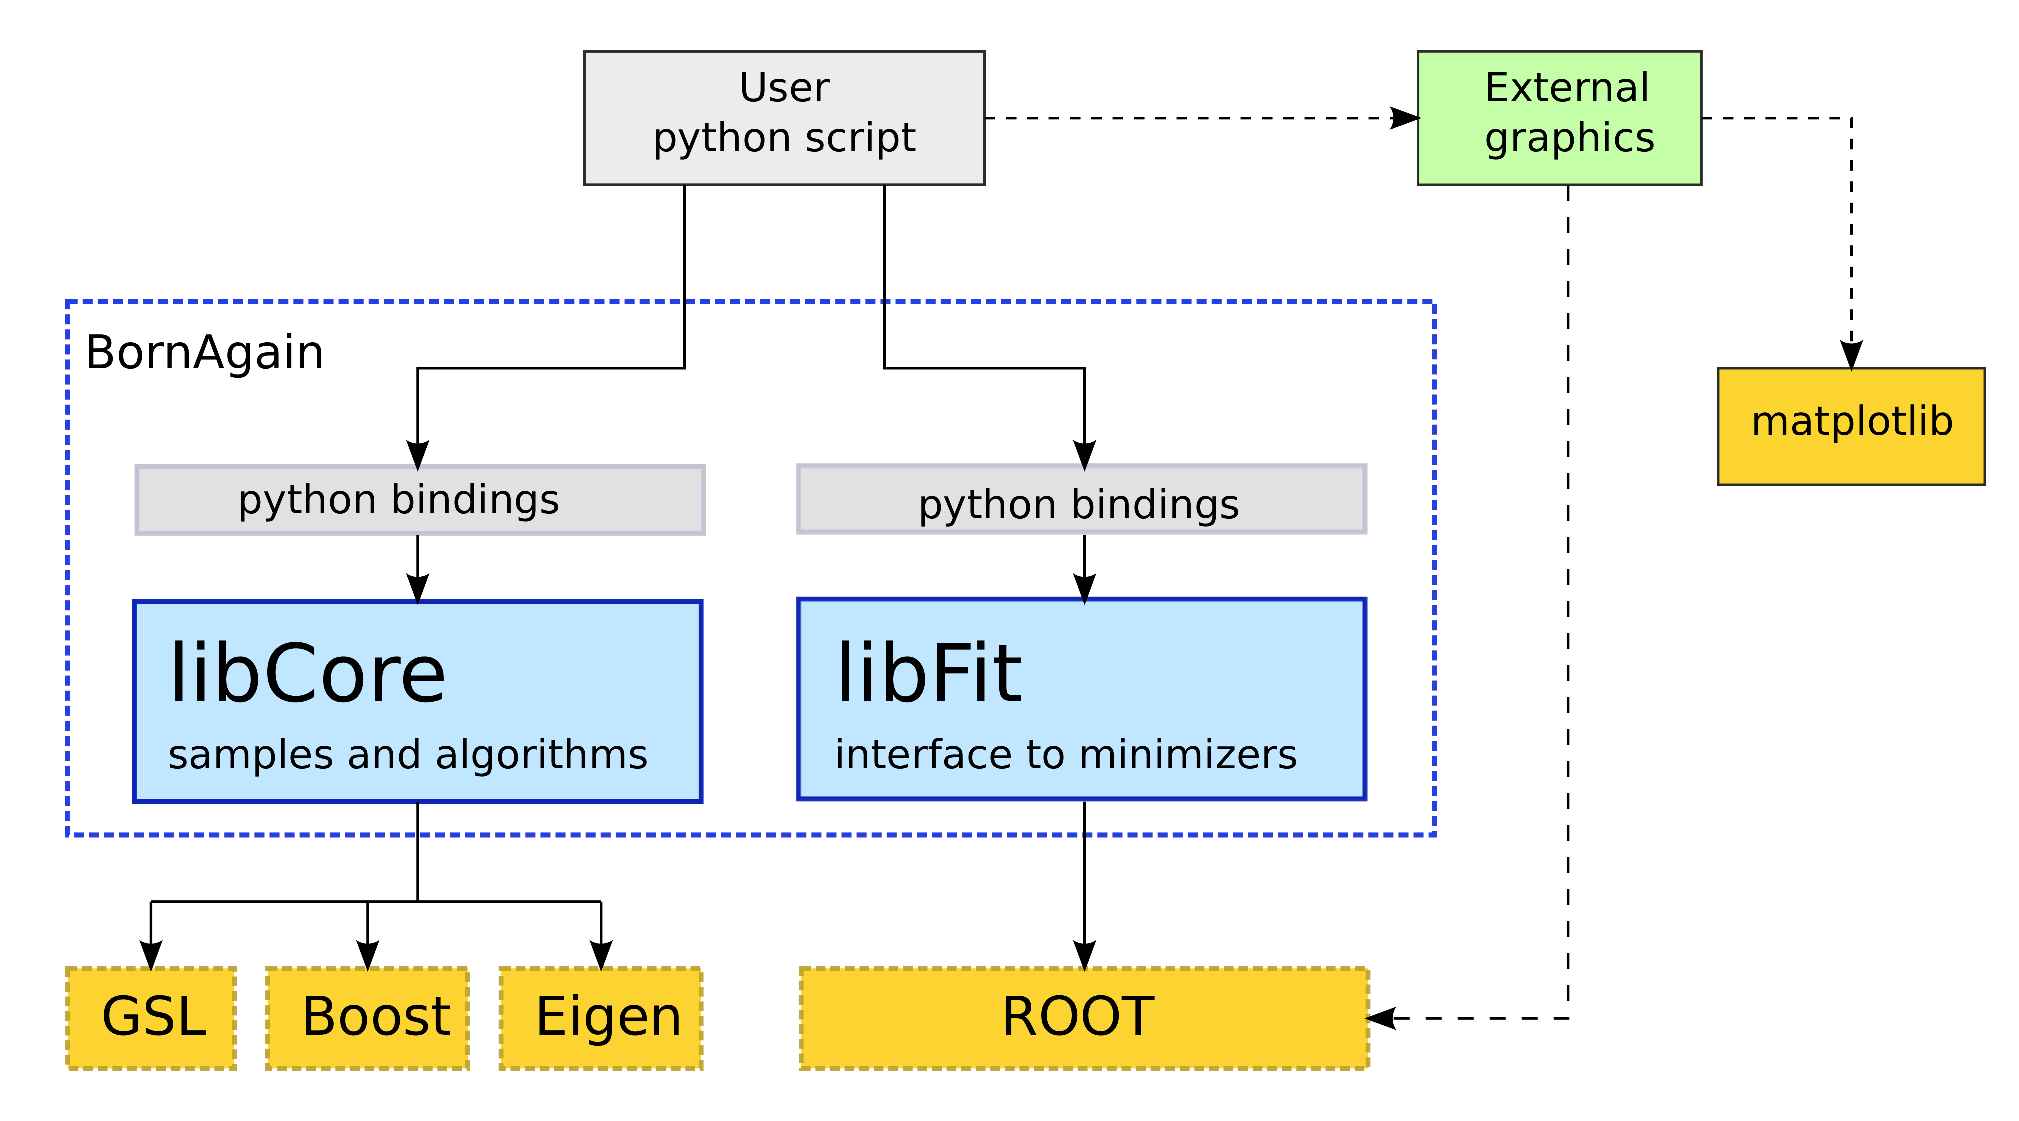
\includegraphics{Figures/basic_architecture.eps}}
\caption{
Structure of \BornAgain\ libraries.
}
\label{fig:two_ratios}
\end{figure}


The general structure of \BornAgain\ and the way user interacts with it are
shown in Fig.~\ref{fig:two_ratios}.
The framework kernel consists of two shared libraries, \Code{libCore} and
\Code{libFit}. Thanks to the python interface they can be imported to the python as external modules. The library \Code{libCore} contains a number of classes, grouped into several class categories necessary for the description of model and running the simulation.
The library  \Code{libFit} contains a number of minimization engines 
and interfaces to them, to let user to fit real data with the model defined.

\BornAgain\ depends from a few external well established open-source libraries: boost, GNU scientific library, Eigen and Fast Fourier Transformation libraries. They are required to be present on the system to run \BornAgain . Other libraries shown
on the plot (ROOT, matplotlib) are optional.

 



\section{Design overview}

% general considerations
% general capabilities and properties
% openess 
% global structure
% design and architecture

% Software process
% - configuration and release management
% - quality assurance and testing
% - user support process


% The BornAgain framework provides a number of classes, grouped into several class categories.


%%%%%%%%%%%%%%%%%%%%%%%%%%%%%%%%%%%%%%%%%%%%%%%%%%%%%%%%%%%%%%%%%%%%%%%%%%%%%%%%%
%%
%%   BornAgain User Manual
%%
%%   homepage:   http://www.bornagainproject.org
%%
%%   copyright:  Forschungszentrum Jülich GmbH 2015
%%
%%   license:    Creative Commons CC-BY-SA
%%   
%%   authors:    Scientific Computing Group at MLZ Garching
%%               C. Durniak, M. Ganeva, G. Pospelov, W. Van Herck, J. Wuttke
%%
%%%%%%%%%%%%%%%%%%%%%%%%%%%%%%%%%%%%%%%%%%%%%%%%%%%%%%%%%%%%%%%%%%%%%%%%%%%%%%%%


\section{Data classes for simulations and fits}

This section will give an overview of the classes that are used to describe all the data needed to perform a single simulation. The prime elements of this data are formed by the sample, the experimental conditions (beam and detector parameters) and simulation parameters.

These classes constitute the main interface to the software's users, since they will mostly be interacting with the program by creating samples and running simulations with specific parameters. Since it is not the intent to explain internals of classes in this document, the text and figures will only mention the most important methods and fields of the classes discussed. Furthermore, getters and setters of private member fields will not be indicated, although these do belong to the public interface. For more detailed information about the project's classes, their methods and fields, the reader is referred to the source code documentation. REF?



\subsection{The Experiment object}
The \Code{Experiment} class holds all references to data objects that are needed to perform a simulation. These consist in a sample description, possibly implemented by a builder object, detector and beam parameters and finally, a simulation parameter class that defines the different approximations that can be used during a simulation. Besides getters and setters for these fields, the class also contains a \Code{runSimulation()} method that will generate an ISimulation object that will perform the actual computations. The class diagram for \Code{Experiment} is shown in \reffig{exp}.

\vspace{8mm}
\begin{figure}[H]
%the makebox macro ensures centering of the resulting figure
\makebox[\textwidth][c]{
\begin{tikzpicture}
\begin{umlpackage}{Simulation Data}
\umlclass{Experiment}{
  -- mp\_sample : ISample* \\
  -- mp\_sample\_builder : ISampleBuilder* \\
  -- m\_detector : Detector \\
  -- m\_beam : Beam \\
  -- m\_intensity\_map : OutputData<double> \\
  -- m\_sim\_params : SimulationParameters
}{
  \umlvirt{+ clone() : Experiment*} \\
  \umlvirt{+ runSimulation() : void} \\
  \umlvirt{+ normalize() : void}
}
\umlemptyclass[x=7, y=0]{ISample}
\umlemptyclass[x=7, y=-2]{Detector}
\umlemptyclass[x=7, y=-4]{Beam}
\umlemptyclass[x=7, y=-6]{SimulationParameters}
\umlemptyclass[y=-4]{GISASExperiment}
\umluniassoc[geometry=|-, anchor1=0]{Experiment}{ISample}
\umluniassoc[geometry=|-, anchor1=0]{Experiment}{Detector}
\umluniassoc[geometry=|-, anchor1=0]{Experiment}{Beam}
\umluniassoc[geometry=|-, anchor1=0]{Experiment}{SimulationParameters}
\umlinherit[geometry=--]{GISASExperiment}{Experiment}

\umlnote[y=-6.5, width=6cm]{GISASExperiment}{
  The ``runSimulation()'' method retrieves an ISimulation object
  from the topmost ISample object and calls its ``run()'' method 
  to perform the actual computations.
}
\end{umlpackage}
\end{tikzpicture}
} %end makebox
\caption{The Experiment class as a container for sample, beam, detector and simulation parameters.}
\label{fig:exp}
\end{figure}

\subsection{The ISample class hierarchy}

Samples are described by a hierarchical tree of objects which all adhere to the ISample interface. The composite pattern is used to achieve a common interface for all objects in the sample tree. The sample description is maximally decoupled from all computational classes, with the exception of the ``createDWBASimulation()'' method. This method will create a new object of type ``DWBASimulation'' that is capable of calculating the scattering contributions originating from the sample part in question. This coupling is not very tight however, since the ISample subclasses only need to know about which class to instantiate and return.

This interface and two of its subclasses are sketched in \reffig{isample}.

\vspace{8mm}

\begin{figure}[H]
\makebox[\textwidth][c]{
\begin{tikzpicture}
\begin{umlpackage}{Sample description} 
% Code from official documentation goes here...
\umlinterface{ISample}{
}{
  \umlvirt{+ clone() : ISample*} \\
  \umlvirt{+ createDWBASimulation() : DWBASimulation*}
}
\umlclass[y=-4]{MultiLayer}{
  -- m\_layers : std::vector<Layer *> \\
  -- m\_interfaces : std::vector<LayerInterface *>
}{
  + getNumberOfLayers() : size\_t \\
  + getNumberOfInterfaces() : size\_t \\
  + addLayer(const Layer \&layer) : void
}
\umlclass[x=8,y=-4]{Layer}{
  -- mp\_material : IMaterial* \\
  -- m\_thickness : double
}{
  + getThickness() : double \\
  + setThickness(double thickness) : void
}
\umlinherit[geometry=-|]{MultiLayer}{ISample}
\umlinherit[geometry=|-]{Layer}{ISample}
\umluniassoc[geometry=--, mult2=n]{MultiLayer}{Layer}
\end{umlpackage}
\end{tikzpicture}
}
\caption{The ISample interface}
\label{fig:isample}
\end{figure}



\subsection{The FitSuite class} \SecLabel{FitSuiteClass}

\subsection{The IMinimizer class} \SecLabel{IMinimizerClass}

\subsection{The MinimizerOptions class} \SecLabel{MinimizerOptionsClass}



\appendix
\addtocontents{toc}{\protect\setcounter{tocdepth}{1}}
%\addtocontents{lof}{\protect\setcounter{tocdepth}{2}}
%%\newpage{\pagestyle{empty}\cleardoublepage}


\chapter{Listings}

%%%%%%%%%%%%%%%%%%%%%%%%%%%%%%%%%%%%%%%%%%%%%%%%%%%%%%%%%%%%%%%%%%%%%%%%%%%%%%%%%%%%%%%%%%%%%%%%%%
%
%%%%%%%%%%%%%%%%%%%%%%%%%%%%%%%%%%%%%%%%%%%%%%%%%%%%%%%%%%%%%%%%%%%%%%%%%%%%%%%%%%%%%%%%%%%%%%%%%%
\section{Python simulation example} \label{PythonSimulationExampleScript}
The following script can be found at
\begin{lstlisting}[language=shell, style=commandline]
./Examples/python/simulation/ex001_CylindersAndPrisms/CylindersAndPrisms.py
\end{lstlisting}


\begin{lstlisting}[
language=python, 
style=eclipse, 
escapeinside={@}{@},
frame = leftline, 
rulecolor = \color{lightgrey},
breaklines = true
]
import numpy
import matplotlib
import pylab
from libBornAgainCore import *


def get_sample():
    """
    Build and return the sample representing cylinders and pyramids on top of
    substrate without interference.
    """
    # defining materials
    m_air = HomogeneousMaterial("Air", 0.0, 0.0)
    m_substrate = HomogeneousMaterial("Substrate", 6e-6, 2e-8)
    m_particle = HomogeneousMaterial("Particle", 6e-4, 2e-8)

    # collection of particles
    cylinder_ff = FormFactorCylinder(5*nanometer, 5*nanometer)
    cylinder = Particle(m_particle, cylinder_ff)
    prism_ff = FormFactorPrism3(10*nanometer, 5*nanometer)
    prism = Particle(m_particle, prism_ff)
    particle_layout = ParticleLayout()
    particle_layout.addParticle(cylinder, 0.0, 0.5)
    particle_layout.addParticle(prism, 0.0, 0.5)
    interference = InterferenceFunctionNone()
    particle_layout.addInterferenceFunction(interference)

    # air layer with particles and substrate form multi layer
    air_layer = Layer(m_air)
    air_layer.setLayout(particle_layout)
    substrate_layer = Layer(m_substrate, 0)
    multi_layer = MultiLayer()
    multi_layer.addLayer(air_layer)
    multi_layer.addLayer(substrate_layer)
    return multi_layer


def get_simulation():
    """
    Create and return GISAXS simulation with beam and detector defined
    """
    simulation = Simulation()
    simulation.setDetectorParameters(100, -1.0*degree, 1.0*degree, 100, 0.0*degree, 2.0*degree)
    simulation.setBeamParameters(1.0*angstrom, 0.2*degree, 0.0*degree)
    return simulation


def run_simulation():
    """
    Run simulation and plot results
    """
    sample = get_sample()
    simulation = get_simulation()
    simulation.setSample(sample)
    simulation.runSimulation()
    result = simulation.getIntensityData().getArray() + 1  # for log scale
    pylab.imshow(numpy.rot90(result, 1), norm=matplotlib.colors.LogNorm(), extent=[-1.0, 1.0, 0, 2.0])
    pylab.show()


if __name__ == '__main__':
    run_simulation()

\end{lstlisting}


%%%%%%%%%%%%%%%%%%%%%%%%%%%%%%%%%%%%%%%%%%%%%%%%%%%%%%%%%%%%%%%%%%%%%%%%%%%%%%%%%%%%%%%%%%%%%%%%%%
%
%%%%%%%%%%%%%%%%%%%%%%%%%%%%%%%%%%%%%%%%%%%%%%%%%%%%%%%%%%%%%%%%%%%%%%%%%%%%%%%%%%%%%%%%%%%%%%%%%%
\newpage
\section{Python fitting example} \label{PythonFittingExampleScript}

The following script can be found at
\begin{lstlisting}[language=shell, style=commandline]
./Examples/python/fitting/ex002_FitCylindersAndPrisms/FitCylindersAndPrisms.py
\end{lstlisting}

\begin{lstlisting}[
language=python, 
style=eclipse, 
frame = leftline, 
rulecolor = \color{lightgrey},
breaklines = true
]
from libBornAgainCore import *
from libBornAgainFit import *


def get_sample():
    """
    Build the sample representing cylinders and pyramids on top of substrate without interference.
    """
    # defining materials
    m_air = HomogeneousMaterial("Air", 0.0, 0.0)
    m_substrate = HomogeneousMaterial("Substrate", 6e-6, 2e-8)
    m_particle = HomogeneousMaterial("Particle", 6e-4, 2e-8)

    # collection of particles
    cylinder_ff = FormFactorCylinder(1.0*nanometer, 1.0*nanometer)
    cylinder = Particle(m_particle, cylinder_ff)
    prism_ff = FormFactorPrism3(2.0*nanometer, 1.0*nanometer)
    prism = Particle(m_particle, prism_ff)
    particle_layout = ParticleLayout()
    particle_layout.addParticle(cylinder, 0.0, 0.5)
    particle_layout.addParticle(prism, 0.0, 0.5)
    interference = InterferenceFunctionNone()
    particle_layout.addInterferenceFunction(interference)

    # air layer with particles and substrate form multi layer
    air_layer = Layer(m_air)
    air_layer.setLayout(particle_layout)
    substrate_layer = Layer(m_substrate, 0)
    multi_layer = MultiLayer()
    multi_layer.addLayer(air_layer)
    multi_layer.addLayer(substrate_layer)
    return multi_layer


def get_simulation():
    """
    Create GISAXS simulation with beam and detector defined
    """
    simulation = Simulation()
    simulation.setDetectorParameters(100, -1.0*degree, 1.0*degree, 100, 0.0*degree, 2.0*degree)
    simulation.setBeamParameters(1.0*angstrom, 0.2*degree, 0.0*degree)
    return simulation


def run_fitting():
    """
    run fitting
    """
    sample = get_sample()
    simulation = get_simulation()
    simulation.setSample(sample)

    real_data = IntensityDataIOFactory.readIntensityData('refdata_fitcylinderprisms.txt')
    
    fit_suite = FitSuite()
    fit_suite.addSimulationAndRealData(simulation, real_data)
    fit_suite.initPrint(10)

    # setting fitting parameters with starting values
    fit_suite.addFitParameter("*FormFactorCylinder/height", 4.*nanometer, 0.01*nanometer, AttLimits.lowerLimited(0.01))
    fit_suite.addFitParameter("*FormFactorCylinder/radius", 6.*nanometer, 0.01*nanometer, AttLimits.lowerLimited(0.01))
    fit_suite.addFitParameter("*FormFactorPrism3/height", 4.*nanometer, 0.01*nanometer, AttLimits.lowerLimited(0.01))
    fit_suite.addFitParameter("*FormFactorPrism3/length", 12.*nanometer, 0.02*nanometer, AttLimits.lowerLimited(0.01))

    # running fit
    fit_suite.runFit()
    
    print "Fitting completed."
    fit_suite.printResults()
    print "chi2:", fit_suite.getMinimizer().getMinValue()
    fitpars = fit_suite.getFitParameters()
    for i in range(0, fitpars.size()):
        print fitpars[i].getName(), fitpars[i].getValue(), fitpars[i].getError()

if __name__ == '__main__':
    run_fitting()
\end{lstlisting}


\chapter{Theory} \label{appendixtheory}

\section{Scattering on nanoparticles - Formal treatment} \label{sec:formal}

\subsection{Green operators and the $T$--matrix}

For a particle, governed by the Schr\"odinger equation with Hamiltonian $H = H_0 + V$, the time--independent scattering theory formally consists of solving the eigenvalue equations:

\begin{equation*}
  H\Psi_\alpha = E_\alpha\Psi_\alpha \; ,
\end{equation*}
with $E$ the scalar energy eigenvalue of the eigenstate $\Psi(E)$.\\
If the solutions of the free (or unperturbed) Hamiltonian $H_0$ are known:
\begin{equation*}
  H_0\Psi_{0\alpha} = E_\alpha\Psi_{0\alpha} \; ,
\end{equation*}
one can write the solutions of the full Hamiltonian in terms of these asymptotic states and Green operators:

\begin{align*}
  \Psi^\pm_\alpha &= \Psi_{0\alpha} + G^\pm_0 V \Psi^\pm_\alpha  \\
  & = \Psi_{0\alpha} + G^\pm V  \Psi_{0\alpha} \; ,
\end{align*}

where the Green operators are defined as:
\begin{align*}
  G^\pm_0(E) &= (E-H_0\pm i\epsilon )^{-1}  \\
  G^\pm (E) &= (E-H\pm i\epsilon )^{-1} \; .
\end{align*}
In these equations, the upper index or sign refers to the state corresponding with the free state $\Psi_{0\alpha}$ at time $t\rightarrow - \infty$ (and vice--versa for the lower sign). Since the solutions of the eigenvalue equations, both for the unperturbed as for the full Hamiltonian, are dependent on the energy eigenvalue $E$, the index $\alpha$ is assumed to include this value (and possibly other quantum numbers).

The transition amplitude between two asymptotic states is given by the $S$--matrix elements, defined as:
\begin{align}
  S_{\alpha\beta} &\equiv \braket{\Psi_{0\beta}}{S}{\Psi_{0\alpha}} \nonumber\\
  & \equiv \braketnoop{\Psi_\beta^-}{\Psi_\alpha^+} \; .
  \label{<++>}
\end{align}

The $S$--matrix can be decomposed into a delta function, representing the absence of scattering, and a $T$--matrix that encodes the scattering part, caused by the potential $V$:
\begin{equation*}
  S_{\alpha\beta} = \delta (E_\alpha - E_\beta)\delta_{\alpha\beta} - 2\pi i \delta (E_\alpha - E_\beta) T^\pm_{\alpha\beta} \; ,
\end{equation*}
with
\begin{align*}
  T^+_{\alpha\beta} & = \braket{\Psi_{0\beta}}{V}{\Psi^+_\alpha} \\
  T^-_{\alpha\beta} & = \braket{\Psi^-_\beta}{V}{\Psi_{0\alpha}} \; .
\end{align*}
On the energy shell $E_\alpha = E_\beta$, one has $T^+_{\alpha\beta}= T^-_{\alpha\beta}$, so that both formulations are equivalent.

By expanding the eigenstates $\Psi^\pm_\alpha$ in these equations, the $T$--matrix elements (on--shell) can be expressed as:
\begin{equation*}
  T^\pm_{\alpha\beta} = V + VG^+ V \; .
\end{equation*}


\subsection{Momentum representation and the scattering cross--section}
The previous general formulas can also be presented in a momentum (and positon) eigenbasis, defined by:
\begin{align*}
  \oper{P}\ket{\vect{k}} & = \hbar \vect{k} \ket{\vect{k}} \\
  \braketnoop{\vect{k'}}{\vect{k}} & = \delta(\vect{k'}-\vect{k}) \\
  1 &= \int d^3\vect{k} \ket{\vect{k}} \bra{\vect{k}} \\
  1 &= \int d^3\vect{r} \ket{\vect{r}} \bra{\vect{r}} \\
  \braketnoop{\vect{r}}{\vect{k}} &= (2\pi)^{-3/2} \exp (i\vect{k}\cdot\vect{r}) \; ,
\end{align*}
where the normalization in the last equation follows from the other definitions.

The wavefunction that evolves from a momentum eigenstate $\ket{\vect{k}_i}$ can then be written as:
\begin{equation*}
  \braketnoop{\vect{r}}{\Psi^+} = \braketnoop{\vect{r}}{\vect{k}_i} + \braket{\vect{r}}{G_0^+T}{\vect{k}_i} \; ,
\end{equation*}
which in the far--field limit becomes:
\begin{align*}
  \braketnoop{\vect{r}}{\Psi^+} &= (2\pi)^{-3/2}\left[ e^{i\vect{k}_i\cdot\vect{r}} - \frac{4\pi^2m}{\hbar^2}\cdot\frac{e^{ik_f r}}{r} \braket{\vect{k}_f}{T}{\vect{k}_i} \right]  \\
  &\equiv (2\pi)^{-3/2}\left[ e^{i\vect{k}_i\cdot\vect{r}} + f(\theta,\phi)\frac{e^{ik_f r}}{r} \right] \; ,
\end{align*}
where the scattering amplitude was defined as
\begin{equation*}
  f(\theta, \phi) = -\frac{4\pi^2m}{\hbar^2}\braket{\vect{k}_f}{T}{\vect{k}_i} \; .
\end{equation*}

The amount of particles per unit time that are scattered in a small solid angle $d\Omega$ in direction $\vect{k}_f$ will then be (still in the far--field limit):
\begin{equation*}
  dI_{scat} = J_0\lvert f(\theta,\phi)\rvert^2d\Omega \; ,
\end{equation*}
where $J_0$ denotes the incident flux density. The scattering cross--section is defined as:
\begin{equation*}
  \frac{d\sigma}{d\Omega}\equiv \frac{dI_{scat}}{J_0 d\Omega} = \lvert f(\theta,\phi) \rvert^2 \; .
\end{equation*}
%%%%%%%%%%%%%%%%%%%%%%%%%%%%%%%%%%%%%%%%%%%
\section{Small angle approximation}
In the case of pure nuclear scattering, the Hamiltonian describing a neutron in a scattering experiment, is given by $H = -\dfrac{\hbar^2}{2m}\Delta + V$, where

\begin{equation*}
  V = \frac{2\pi \hbar^2}{m}\rho_s(\vect{r}) \; ,
\end{equation*}
with $\rho_s(\vect{r})$ the scattering length density of the sample. This scattering length density typically consists of a sum of weighted delta--functions, peaked at the atomic postions of the sample. For small scattering angles, the Bragg condition will not be fulfilled and the scattering length density may be replaced by a continuous function, representing the average scattering length density. In this case, one can define a refractive index, which in general will also be a continuous function of the position in the sample:
\begin{equation*}
  n^2(\vect{r}) \equiv 1 - \frac{4\pi}{k_0^2}\rho_s(\vect{r}) \; ,
\end{equation*}
with $k_0$ the wavevector in vacuum, or alternatively $k_0 = 2\pi /\lambda$, with $\lambda$ the de Broglie wavelength of the neutron.


Substituting this refractive index in the potential then gives:
\begin{equation*}
  V(\vect{r}) = \frac{\hbar^2}{2m}k_0^2(1-n^2(\vect{r})) \; .
\end{equation*}

Using these definitions, one can rescale the Hamiltonian with a factor $2m/\hbar^2$, such that
\begin{align*}
  \widetilde{H} &\equiv -\Delta + \widetilde{V} \nonumber \\
  \widetilde{V}(\vect{r}) &\equiv 4\pi\rho_s(\vect{r}) = k_0^2(1-n^2(\vect{r})) \; .
\end{align*}
It should be noted that this Hamiltonian implicitly contains the energy eigenvalue ($E_{k_0}=(\hbar k_0)^2/2m$), so that it can only be used in the time--independent Schr\"odinger equation $H\Psi_\alpha = E_\alpha \Psi_\alpha$.

The $T$--matrix then also becomes rescaled and the scattering amplitude becomes:
\begin{equation*}
  f(\theta, \phi) = -2\pi^2 \braket{\vect{k}_f}{\widetilde{T}}{\vect{k}_i} \; .
\end{equation*}

%%%%%%%%%%%%%%%%%%%%%%%%%%%%%%%%%%
\section{Born approximation} \label{sec:ba}
Consider a scattering volume $V$, containing $N$ scattering centers with shape functions $S^i(\vect{r})$, positions $\vect{R}^i$ and scattering length density $\rho_s$ (relative to the ambient material).

In the Born approximation ($\widetilde{T}\simeq\widetilde{V}$), the scattering amplitude is
\begin{align*}
  f(\theta, \phi) & = -8\pi^3 \braket{\vect{k_f}}{\rho_s(\vect{r})}{\vect{k_i}} \nonumber \\
  & = -\int d^3\vect{r} e^{i\vect{q}\cdot\vect{r}} \rho_s(\vect{r}) \; ,
\end{align*}
where $\vect{q}\equiv \vect{k}_i - \vect{k}_f$ denotes the wavevector transfer and
\begin{equation*}
  \rho_s(\vect{r}) = \frac{k_0^2}{4\pi}(1-n^2(\vect{r})) \; .
\end{equation*}

The differential cross--section (per scattering center) is then given by:
\begin{equation*}
  \frac{d\sigma}{d\Omega}(\vect{q}) = \frac{1}{N}\left\lvert \int_V \rho_s(\vect{r}) e^{i\vect{q}\cdot\vect{r}} d^3\vect{r} \right\rvert ^2 \; .
\end{equation*}

Following the initial assumptions. the scattering length density can be written as:
\begin{equation*}
\rho_s(\vect{r}) = \sum_i \rho_{s,i} S^i(\vect{r}) \otimes \delta (\vect{r}-\vect{R}^i) \; ,
\end{equation*}
with $\rho_{s,i}$ the scattering length density of particle $i$. The cross--section then becomes:
\begin{align*}
  N\frac{d\sigma}{d\Omega}(\vect{q}) & = \left\lvert \sum_i F^i(\vect{q}) \exp (i\vect{q}\cdot\vect{R}^i) \right\rvert ^2  \\
  & = \left\lbrace \sum_i \left\lvert F^i(\vect{q}) \right\rvert ^2 + \sum_{i\neq j} F^i(\vect{q}) F^{j*}(\vect{q}) \exp \left[i\vect{q}\cdot (\vect{R}^i-\vect{R}^j)\right] \right\rbrace \; .
\end{align*}
In the last expression, the formfactors $F^i(\vect{q})$ are the Fourier transforms of the shape functions, including their scattering length densities:
\begin{equation*}
  F^i(\vect{q}) \equiv \int_V d^3\vect{r} \rho_{s,i} S^i(\vect{r}) \exp (i\vect{q}\cdot\vect{r} ) \; .
\end{equation*}


Since in most real conditions only the statistical properties of the particles are known, one can consider the expectation value of this cross--section. Assuming that the particles' shapes are determined by their class $\alpha$, with abundance ratio $p_\alpha \equiv N_\alpha / N$, and defining the particle density $\rho_V \equiv N/V$, the expectation value becomes:
\begin{align*}
  \left\langle \frac{d\sigma}{d\Omega}(\vect{q}) \right\rangle  & = \sum_\alpha p_\alpha \left\lvert F_\alpha(\vect{q})\right\rvert ^2 + \frac{\rho_V}{V}\sum_{\alpha,\beta} p_\alpha p_\beta F_\alpha (\vect{q})F_\beta^*(\vect{q})  \\
  & \times \iint_V d^3\vect{R}_\alpha d^3\vect{R}_\beta \ppcf{\alpha}{\beta}{R} \exp \left[ i\vect{q}\cdot (\vect{R}_\alpha - \vect{R}_\beta ) \right] \; .
\end{align*}

In this equation, the factor $\ppcf{\alpha}{\beta}{R}$ is called the \emph{partial pair correlation function} and it represents a normalized probability of finding particles of type $\alpha$ and $\beta$ in positions $\vect{R}_\alpha$ and $\vect{R}_\beta$ respectively. More precisely, the probability density for finding a particle $\alpha$ at position $\vect{R}_\alpha$ and another one of type $\beta$ at $\vect{R}_\beta$ is given by:
\begin{equation*}
  \mathcal{P}(\alpha, \vect{R}_\alpha ; \beta , \vect{R}_\beta ) \equiv \rho_V^2 p_\alpha p_\beta \ppcf{\alpha}{\beta}{R} \; .
\end{equation*}

\subsection{General formulas}
Even in the most general case, the partial pair correlation function will only depend on the difference $\vect{R}_{\alpha\beta}\equiv(\vect{R}_\alpha - \vect{R}_\beta )$ of the particles' positions. One of the volume integrals can then be dropped, together with the volume factor, giving:
\begin{align*}
  \left\langle \frac{d\sigma}{d\Omega}(\vect{q}) \right\rangle  & = \sum_\alpha p_\alpha \left\lvert F_\alpha(\vect{q})\right\rvert ^2 + \rho_V\sum_{\alpha,\beta} p_\alpha p_\beta F_\alpha (\vect{q})F_\beta^*(\vect{q}) \\
  & \times \int_V d^3\vect{R}_{\alpha\beta} \ppcfb{\alpha}{\beta}{R} \exp \left[ i\vect{q}\cdot \vect{R}_{\alpha\beta} \right] \; .
\end{align*}

This expression can be split into a diffuse part, which by definition should be zero for the case of only one particle type, and a coherent part, resulting from the coherent superposition of scattering amplitudes for particles at different positions:
\begin{equation*}
  \left\langle \frac{d\sigma}{d\Omega}(\vect{q}) \right\rangle = I_d(\vect{q}) + \ensavg{\alpha\beta}{F_\alpha (\vect{q} ) S_{\alpha\beta} (\vect{q}) F_\beta^* (\vect{q})} \; ,
\end{equation*}
where
\begin{align*}
  I_d(\vect{q}) &\equiv \ensavg{\alpha}{\left\rvert F_\alpha (\vect{q}) \right\rvert^2} - \left\lvert \ensavg{\alpha}{ F_\alpha (\vect{q})} \right\rvert^2 \; , \\
  S_{\alpha\beta} (\vect{q}) &\equiv 1 + \rho_V \int_V d^3\vect{R}_{\alpha\beta}\ppcfb{\alpha}{\beta}{R} \exp \left[ i\vect{q}\cdot \vect{R}_{\alpha\beta} \right] \; .
\end{align*}
$S_{\alpha\beta} (\vect{q})$ is called the \emph{interference function} and $\langle\dotso\rangle_\alpha$ is the expectation value over the classes $\lbrace \alpha\rbrace$.

\subsection{Decoupling approximation}
When the partial pair correlation function is independent of the particle class $\alpha$ ($ \ppcfb{\alpha}{\beta}{R} \equiv g(\vect{R}_{\alpha\beta})$ ), the scattering cross--section becomes:
\begin{equation*}
\left\langle \frac{d\sigma}{d\Omega}(\vect{q}) \right\rangle  = I_d(\vect{q}) + \left\lvert \left\langle F_\alpha(\vect{q}) \right\rangle_\alpha \right\rvert ^2 \times S(\vect{q}) \; ,
\end{equation*}
where
\begin{equation*} 
  S(\vect{q}) = 1+ \rho_V \int_V d^3\vect{R} \; g(\vect{R}) \exp \left[ i\vect{q}\cdot \vect{R} \right] \; .
\end{equation*}

\subsection{Local Monodisperse Approximation}
By assuming that inside every coherence region of the beam, the particle class (or size/shape) is fixed, the cross--section will consist of an incoherent superposition of these different coherence regions and can be written as:
\begin{equation*}
  \left\langle \frac{d\sigma}{d\Omega}(\vect{q}) \right\rangle \simeq \left\langle \left\lvert F_\alpha(\vect{q})\right\rvert ^2 S_\alpha(\vect{q}) \right\rangle_\alpha \; .
\end{equation*}

Contrary to the Decoupling Approximation, the Local Monodisperse Approximation can account for particle class/size/shape--dependent pair correlation functions by having distinct interference functions $S_\alpha(\vect{q})$.

%%%%%%%%%%%%%%%%%%%%%%%%%%%%%%%%%%%%%%%%%%%
\subsection{Size--Spacing Correlation Approximation}
In the Size--Spacing Correlation Approximation, a correlation is assumed between the shape/size of the particles and their mutual spacing. A classical example would consist of particles whose closest--neighbour spacing depends linearly on the sum of their respective sizes. The following discussion of this type of correlation is inspired by \cite{LaLe07}

The scattered intensity can also be calculated as the Fourier transform of the Patterson function, which is the autocorrelation of the scattering length density:
\begin{equation*}
  \curlp (\vectr ) \equiv \sum_{ij} S_i(-\vectr )\otimes S_j(\vectr )\otimes \delta (\vectr + \vectr_i - \vectr_j ) \; .
\end{equation*}
For a sample where only the statistical properties of particle positions and shape/size are known, the scattered intensity per scattering particle becomes average over an ensemble of the Fourier transform of the Patterson function:
\begin{equation*}
  I(\vectq ) = \frac{1}{N}\ensavg{}{\curlf (\curlp (\vectr ))} \; ,
\end{equation*}
where $\curlf$ denotes the Fourier transform.

The ensemble averaged Patterson function will be denoted as:
\begin{equation*}
  Z(r) \equiv \frac{1}{N}\ensavg{}{\curlp (\vectr )} \; .
\end{equation*}
In the case of systems where the particles are aligned in one dimension, this autocorrelation function can be further split into nearest neighbour probabilities. First, it is split into terms for negative, zero or positive distance:
\begin{equation*}
  Z(\vectr ) \equiv z_0(\vectr ) + z_+(\vectr ) + z_-(\vectr ) \; .
\end{equation*}
Taking $x$ as the coordinate in the direction in which the particles are arranged and $s$ as an orthogonal coordinate ($\vectr \equiv (x,s)$), one obtains:
\begin{align*}
  z_0(\vectr ) &= \sum_{\alpha_0} p(\alpha_0) S_{\alpha_0}(-x,-s) \otimes S_{\alpha_0}(x,s)  \\
  z_+(\vectr ) &= \sum_{\alpha_0\alpha_1} p(\alpha_0,\alpha_1) S_{\alpha_0}(-x,-s) \otimes S_{\alpha_1}(x,s) \otimes P_1(x|\alpha_0\alpha_1)  \\
               &+ \sum_{\alpha_0\alpha_1\alpha_2} p(\alpha_0,\alpha_1,\alpha_2) S_{\alpha_0}(-x,-s) \otimes S_{\alpha_2}(x,s) \otimes P_1(x|\alpha_0\alpha_1) \otimes P_2(x|\alpha_0\alpha_1\alpha_2)  \\
               &+ \dotsb \\
  z_-(\vectr ) &= z_+(-\vectr ) \; ,
\end{align*}
where $p(\alpha_0,\dotsc ,\alpha_n)$ denotes the probability of having a sequence of particles of the indicated sizes/shapes and $P_n(x|\alpha_0\dotsc\alpha_n)$ is the probability density of having a particle of type $\alpha_n$ at a (positive) distance $x$ of its nearest neighbour of type $\alpha_{n-1}$ in a sequence of the given order.



In the Size--Spacing Correlation Approximation, one assumes that the particle sequence probabilities are just a product of their individual fractions:
\begin{equation*}
  p(\alpha_0,\dotsc ,\alpha_n) = \prod_i p(\alpha_i) \; ,
\end{equation*}
and the nearest neighbour distance distribution is dependent only on the two particles involved:
\begin{equation*}
  P_n(x|\alpha_0\dotsc\alpha_n) = P_1(x|\alpha_{n-1}\alpha_n) \; .
\end{equation*}
Furthermore, the distance distribution $P_1(x|\alpha_0\alpha_1)$ depends on the particle sizes/shapes only through its mean value $D$:
\begin{equation*}
  P_1(x|\alpha_0\alpha_1) = P_0(x - D(\alpha_0,\alpha_1) ) \; ,
\end{equation*}
where $D(\alpha_0,\alpha_1) = D_0 + \kappa \left[ \Delta R(\alpha_0) + \Delta R(\alpha_1) \right]$, with $\Delta R(\alpha_i)$ the deviation of a size parameter of particle $i$ with respect to the mean over all particles sizes/shapes and $\kappa$ the coupling parameter.

In momentum space, the sum of convolutions can be written as a geometric series, which can be exactly calculated to be:
\begin{equation}
\label{eq:sscainf}
  I(\vectq ) = \ensavg{\alpha}{\left| F_\alpha(\vectq ) \right| ^2} + 2 \Re \left\lbrace \widetilde{\curlf_\kappa}(\vectq )\widetilde{\curlf_\kappa^*}(\vectq ) \cdot \frac{\Omega_\kappa(\vectq )}{\tilde{p}_{2\kappa}(\vectq )\left[ 1 - \Omega_\kappa(\vectq )\right] } \right\rbrace \; ,
\end{equation}
with
\begin{align*}
  \tilde{p}_\kappa(\vectq ) &= \int d\alpha\; p(\alpha) e^{i\kappa q_x \Delta R(\alpha)}  \\
  \Omega_\kappa(\vectq ) &= \tilde{p}_{2\kappa}(\vectq ) \phi(\vectq) e^{i q_x D_0}  \\
  \widetilde{\curlf_\kappa}(\vectq ) &= \int d\alpha\; p(\alpha)F_\alpha (\vectq ) e^{i\kappa q_x \Delta R(\alpha)} \; ,
\end{align*}
and the Fourier transform of $P_1(x|\alpha_0\alpha_1)$ is
\begin{equation*}
  \curlp (\vectq ) = \phi (\vectq )e^{i q_x D_0} e^{i \kappa q_x \left[ \Delta R(\alpha_0) + \Delta R(\alpha_1) \right] } \; .
\end{equation*}

Using the result from the one--dimensional analysis, one can apply this formula ad hoc for distributions of particles in a plane, where the coordinate $x$ will now be replaced with $(x,y)$, while the $s$ coordinate encodes a position in the remaining orthogonal direction. One must be aware however that this constitutes a further approximation, since this type of correlation does not have a general solution in more than one dimension.

The intensity in \refeq{sscainf} will contain a Dirac delta function contribution, caused by taking an infinite sum of terms that are perfectly correlated at $\vectq = 0$. One can leverage this behaviour by multiplying the nearest neighbour distribution by a constant factor $e^{-D/\Lambda}$, which removes the division by zero in \refeq{sscainf}.
Another way of dealing with this infinity at $\vectq =0$ consists of taking only a finite number of terms, in which case the geometric series still has an analytical solution, but becomes a bit more cumbersome:
\begin{equation*}
\begin{split}
  I(\vectq ) &= \ensavg{\alpha}{\left| F_\alpha(\vectq ) \right| ^2} + 2 \Re \Biggl\lbrace \frac{1}{\tilde{p}_{2\kappa}(\vectq )}\widetilde{\curlf_\kappa}(\vectq )\widetilde{\curlf_\kappa^*}(\vectq ) \\
  & \times \left[ \left( 1 - \frac{1}{N}\right) \frac{\Omega_\kappa(\vectq )}{1 - \Omega_\kappa(\vectq ) } - \frac{1}{N}\frac{\Omega_\kappa^2(\vectq )\left( 1- \Omega_\kappa^{N-1}(\vectq )\right) }{\left( 1 - \Omega_\kappa(\vectq ) \right) ^2 } \right] \Biggr\rbrace \; .
\end{split}
\end{equation*}
This expression has a well--defined limit for $\Omega_\kappa(\vectq ) \rightarrow 1$ (when $\vectq \rightarrow 0$), namely:
\begin{equation*}
  \lim_{\vectq \rightarrow 0} I(\vectq ) = \ensavg{\alpha}{\left| F_\alpha(0 ) \right| ^2} + \left( N-1 \right) \left| \ensavg{\alpha}{F_\alpha(0 )} \right|^2 \; .
\end{equation*}

%%%%%%%%%%%%%%%%%%%%%%%%%%%%%%%%%%%%%
\section{Distorted Wave Born Approximation} 
In this section, one proceeds along similar lines as in the formal treatment of section \ref{sec:formal}. This time however, the full Hamiltonian is written as $H_2 = H_1 + V_2 = H_0 +V_1 + V_2$, where $H_0$ will again refer to the free Hamiltonian. In the distorted wave Born approximation (DWBA), one performs a perturbative expansion around the solutions of the Hamiltonian $H_1$, which are assumed to be known:
\begin{align*}
  H_1\Psi^\pm_{1\alpha} &= E_\alpha\Psi^\pm_{1\alpha} \\
  \Psi^\pm_{1\alpha} &= \Psi_{0\alpha} + G^\pm_1 V_1 \Psi_{0\alpha} \; ,
\end{align*}
where the Green operators are defined to be:
\begin{align*}
  G^\pm_1 &\equiv (E-H_1\pm i\epsilon) ^{-1} \nonumber \\
  G^\pm_2 &\equiv (E-H_2\pm i\epsilon) ^{-1} \; .
\end{align*}

The $T$--matrix element for scattering between the asymptotic states $\Psi_{0\alpha}$ and $\Psi_{0\beta}$ (note that these asymptotic states refer to the free Hamiltonian $H_0$), is:
\begin{align*}
  T^+_{\alpha\beta} &= \braket{\Psi_{0\beta}}{V_1+V_2}{\Psi^+_\alpha} \nonumber \\
  & = \braket{\Psi_{0\beta}}{V_1+V_2}{\Psi_{0\alpha} + G^+_1V_1\Psi_{0\alpha} + G^+_2V_2\Psi^+_{1\alpha}} \nonumber \\
  & = \braket{\Psi_{0\beta}}{V_1}{\Psi^+_{1\alpha}} + \braket{\Psi_{0\beta}}{(V_1G^+_1 + 1)V_2}{\Psi^+_\alpha} \\
  & = \braket{\Psi_{0\beta}}{V_1}{\Psi^+_{1\alpha}} + \braket{\Psi^-_{1\beta}}{V_2}{\Psi^+_\alpha} \nonumber \\
  & = \braket{\Psi_{0\beta}}{V_1}{\Psi^+_{1\alpha}} + \braket{\Psi^-_{1\beta}}{T_2}{\Psi^+_{1\alpha}} \; ,
\end{align*}
with $T_2 = V_2 + V_2G^+_2V_2$. By approximating this last term using $T_2 \simeq V_2$, one arrives at the distorted wave Born approximation:
\begin{equation*}
  \label{eq:tdwba}
   T^+_{\alpha\beta} \simeq \braket{\Psi_{0\beta}}{V_1}{\Psi^+_{1\alpha}} + \braket{\Psi^-_{1\beta}}{V_2}{\Psi^+_{1\alpha}} \; .
\end{equation*}

%%%%%%%%%%%%%%%%%%%%%%%%%%%%%%%%%%%%%
\subsection{Multilayer systems}
In multilayer systems, the first term of \refeq{tdwba} denotes the specular part of the reflection, while the second term is responsible for the off-specular scattering. This off-specular part is caused by deviations from the perfectly smooth layered system, as e.g. interface roughnesses or included nanoparticles. In here only the case of nanoparticles will be treated.

In the conventions where $H=-\Delta + V$, the potential splits into two parts $V_1$ and $V_2$, where only the second part is treated as a perturbation:
\begin{align*}
  V_1 & = k_0^2\left( 1-n_0^2(\vect{r})\right)  \\
  V_2 & = \sum_i k_0^2\left( n_0^2(\vect{R}^i) - n_i^2 \right) S^i(\vect{r}) \otimes \delta(\vect{r}-\vect{R}^i) \; ,
\end{align*}
where $n_0(\vect{r})$ denotes the refractive index of the unperturbed system (which, in case of a multilayer system, will only depend on its $z$--coordinate) and $n_i$ is the refractive index of the nanoparticle with shape function $S^i$ and position $\vect{R}^i$.

For nanoparticles in a specific layer $j$, i.e. $V_2\neq0$ only in layer $j$, one only needs the unperturbed solutions in layer $j$:
\begin{align*}
  \braketnoop{\vect{r}}{\Psi^+_{1k_i}} &= (2\pi)^{-3/2}\left[ R_j(\vect{k}_i) e^{i \vect{k}_{j,R}(\vect{k}_i)\cdot\vect{r}} + T_j(\vect{k}_i) e^{i \vect{k}_{j,T}(\vect{k}_i)\cdot\vect{r}} \right] \\
  \braketnoop{\Psi^-_{1k_f}}{\vect{r}} &= (2\pi)^{-3/2}\left[ R_j(-\vect{k}_f) e^{i \vect{k}_{j,R}(-\vect{k}_f)\cdot\vect{r}} + T_j(-\vect{k}_f) e^{i \vect{k}_{j,T}(-\vect{k}_f)\cdot\vectr} \right] \; .
\end{align*}

The off--specular contribution to the scattering amplitude then becomes:
\begin{align*}
  f(\theta, \phi) &= -\int d^3\vectr \frac{V_2(\vectr)}{4\pi} \biggl[ T_iT_fe^{i(\vectk_{j,i}-\vectk_{j,f})\cdot\vectr} + R_iT_fe^{i(\vectkt_{j,i}-\vectk_{j,f})\cdot\vectr} \\
   & + T_iR_fe^{i(\vectk_{j,i}-\vectkt_{j,f})\cdot\vectr} + R_iR_fe^{i(\vectkt_{j,i}-\vectkt_{j,f})\cdot\vectr} \biggr] \; ,
\end{align*}
where the following shorthand notations were used:
\begin{align*}
  T_i &\equiv  T_j(\vect{k}_i) & R_i &\equiv  R_j(\vect{k}_i)  \\
  T_f &\equiv  T_j(-\vect{k}_f) & R_f &\equiv  R_j(-\vect{k}_f) \\
  \vectk_{j,i} &\equiv \vectk_{j,T}(\vectk_i) & \vectkt_{j,i} &\equiv \vectk_{j,R}(\vectk_i)  \\
  \vectk_{j,f} &\equiv -\vectk_{j,T}(-\vectk_f) & \vectkt_{j,f} &\equiv -\vectk_{j,R}(-\vectk_f) \; .
\end{align*}

From this expression, one sees that the scattering amplitude consists of a weighted sum of Fourier transforms of the potential $V_2$. Using
\begin{equation*}
  V_2(\vectr) = \sum_i 4\pi \rho_{s,rel,i} S^i(\vectr) \otimes \delta(\vectr - \vect{R}^i) \; ,
\end{equation*}
with $\rho_{s,rel,i}\equiv  k_0^2\left( n_0^2(\vect{R}^i) - n_i^2 \right)/4\pi$, the scattering amplitude becomes
\begin{equation*}
  f(\theta, \phi) = -\sum_i  \rho_{s,rel,i} \curlf^i_{\text{DWBA}}(\vectk_{j,i},\vectk_{j,f},\vect{R}^i_z)e^{i(\vectk_{j,i\parallel}-\vectk_{j,f\parallel})\cdot \vect{R}^{i\parallel} } \; ,
\end{equation*}
with
\begin{align*}
  \curlf^i_\text{DWBA}(\vectk_i,\vectk_f,R_z) & \equiv T_iT_fF^i(\vectk_i-\vectk_f)e^{i(k_{iz}-k_{fz})R_z} + R_iT_fF^i(\vectkt_i-\vectk_f)e^{i(-k_{iz}-k_{fz})R_z} \\
  & + T_iR_fF^i(\vectk_i-\vectkt_f)e^{i(k_{iz}+k_{fz})R_z} + R_iR_fF^i(\vectkt_i-\vectkt_f)e^{i(-k_{iz}+k_{fz})R_z} \; ,
\end{align*}

With this last expression, the same techniques as demonstrated in section \ref{sec:ba} can be applied, leading to the following expression for the expectation value of the scattering cross--section:
\begin{align*}
  & \left\langle \frac{d\sigma}{d\Omega}(\vectk_i,\vectk_f) \right\rangle_{\text{Off--specular}}  \\
  & = \sum_\alpha p_\alpha \left\lvert \curlf_\alpha(\vectk_{j,i},\vectk_{j,f}, R_{\alpha,z})\right\rvert ^2 + \frac{\rho_S}{S}\sum_{\alpha,\beta} p_\alpha p_\beta \curlf_\alpha (\vectk_{j,i},\vectk_{j,f}, R_{\alpha,z})\curlf_\beta^*(\vectk_{j,i},\vectk_{j,f}, R_{\beta,z}) \\
  & \times \iint_S d^2\vect{R}_\alpha^\parallel d^2\vect{R}_\beta^\parallel \ppcf{\alpha}{\beta}{R^\parallel} \exp \left[ i\vect{q}_{j\parallel}\cdot (\vect{R}_\alpha^\parallel - \vect{R}_\beta^\parallel ) \right] \; .
\end{align*}

The main differences with respect to the cross---section in the Born approximation are:
\begin{enumerate}
  \item The particle form factor now consists of a more complex expression and now depends on both incoming and outgoing wavevectors and also on the $z$--coordinate of the particle;
  \item Since the $z$--coordinate of the particles is implicitly included in its formfactor, the position integrals only run over $x$-- and $y$--coordinates and the volume and density gets replaced with the surface area and surface density respectively.
\end{enumerate}


\chapter{Formfactors}

\begin{itemize}
\item Parallelepiped
\item Pyramid
\item Cylinder
\item Cone
\item Prism3
\item Tethraedron
\item Prism6
\item Cone6
\item Cut-off sphere, \SecRef{Sphere} 
\item Cybooctaedron
\item Facetted sphere  
\item Full sphere, \SecRef{FullSphere} 
\item Full spheroid 
\item Box
\item Anisotropic pyramid
\item Ellipsoid
\item Anisotropic hemi-spheroid
\item Spheroid
\end{itemize}

\newpage
\section{Formfactor Cut-off Sphere}\SecLabel{Sphere}
\subsection{Real-space geometry}

A sphere, with a planar cut-off. 
\par
\paragraph{Parameters:}
\begin{itemize}
\item radius $R$
\item heigth $H$
\item volume $V=\pi R^3 \left[\dfrac{2}{3} + \dfrac{H-R}{R} - \dfrac{1}{3}\left(\dfrac{H-R}{R}\right)^3\right]$
\item particle surface seen from above $S = \left\{\begin{array}{ll} \pi R^2, & H > R \\
         \pi\left(2RH-H^2\right), & H < R \end{array}\right. .$
\item gyration radius along $z$ axis $R_g = \left\{\begin{array}{ll}  R, & H > R \\
         \sqrt{2RH-H^2}, & H < R \end{array}\right. .$
\end{itemize}

\paragraph{Restrictions}
\begin{itemize}
\item $H\leq 2R$
\end{itemize}


\par
%\paragraph{Sketch}
\begin{figure}[!h]
\begin{center}
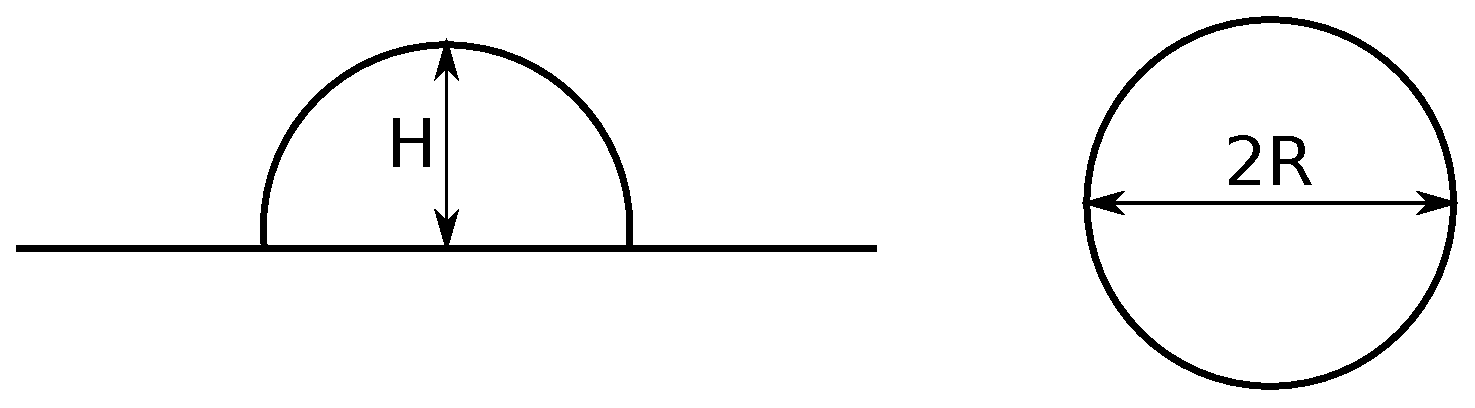
\includegraphics[width=0.6\columnwidth]{Figures/sphere}
\caption{Sketch of the formfactor sphere. Left: front view, right: top view.}
\end{center}
\label{sphere}
\end{figure}

\subsection{Computing the formfactor}
The formfactor can be computed analytically upto a 1-dimensional quadrature:
\begin{equation}
F(\mathbf q, R, H) = \exp\left[iq_z\left(H-R\right)\right]\int\limits_{R-H}^{R}{2\pi R_z^2\frac{J_1(q_{||}R_z)}{q_{||}R_z}\exp\left[iq_zz\right]dz} 
\label{eq:ffsphere}
\end{equation}
with abbreviations
\begin{eqnarray}
q_{||} &=& \sqrt{q_x^2+q_y^2} \\
R_z &=& \sqrt{R^2-z^2} 
\end{eqnarray}

\subsection{Exemplary formfactor}
Computed results for $R=10$~nm and $H=13$~nm.
\begin{figure}[h]
\begin{center}
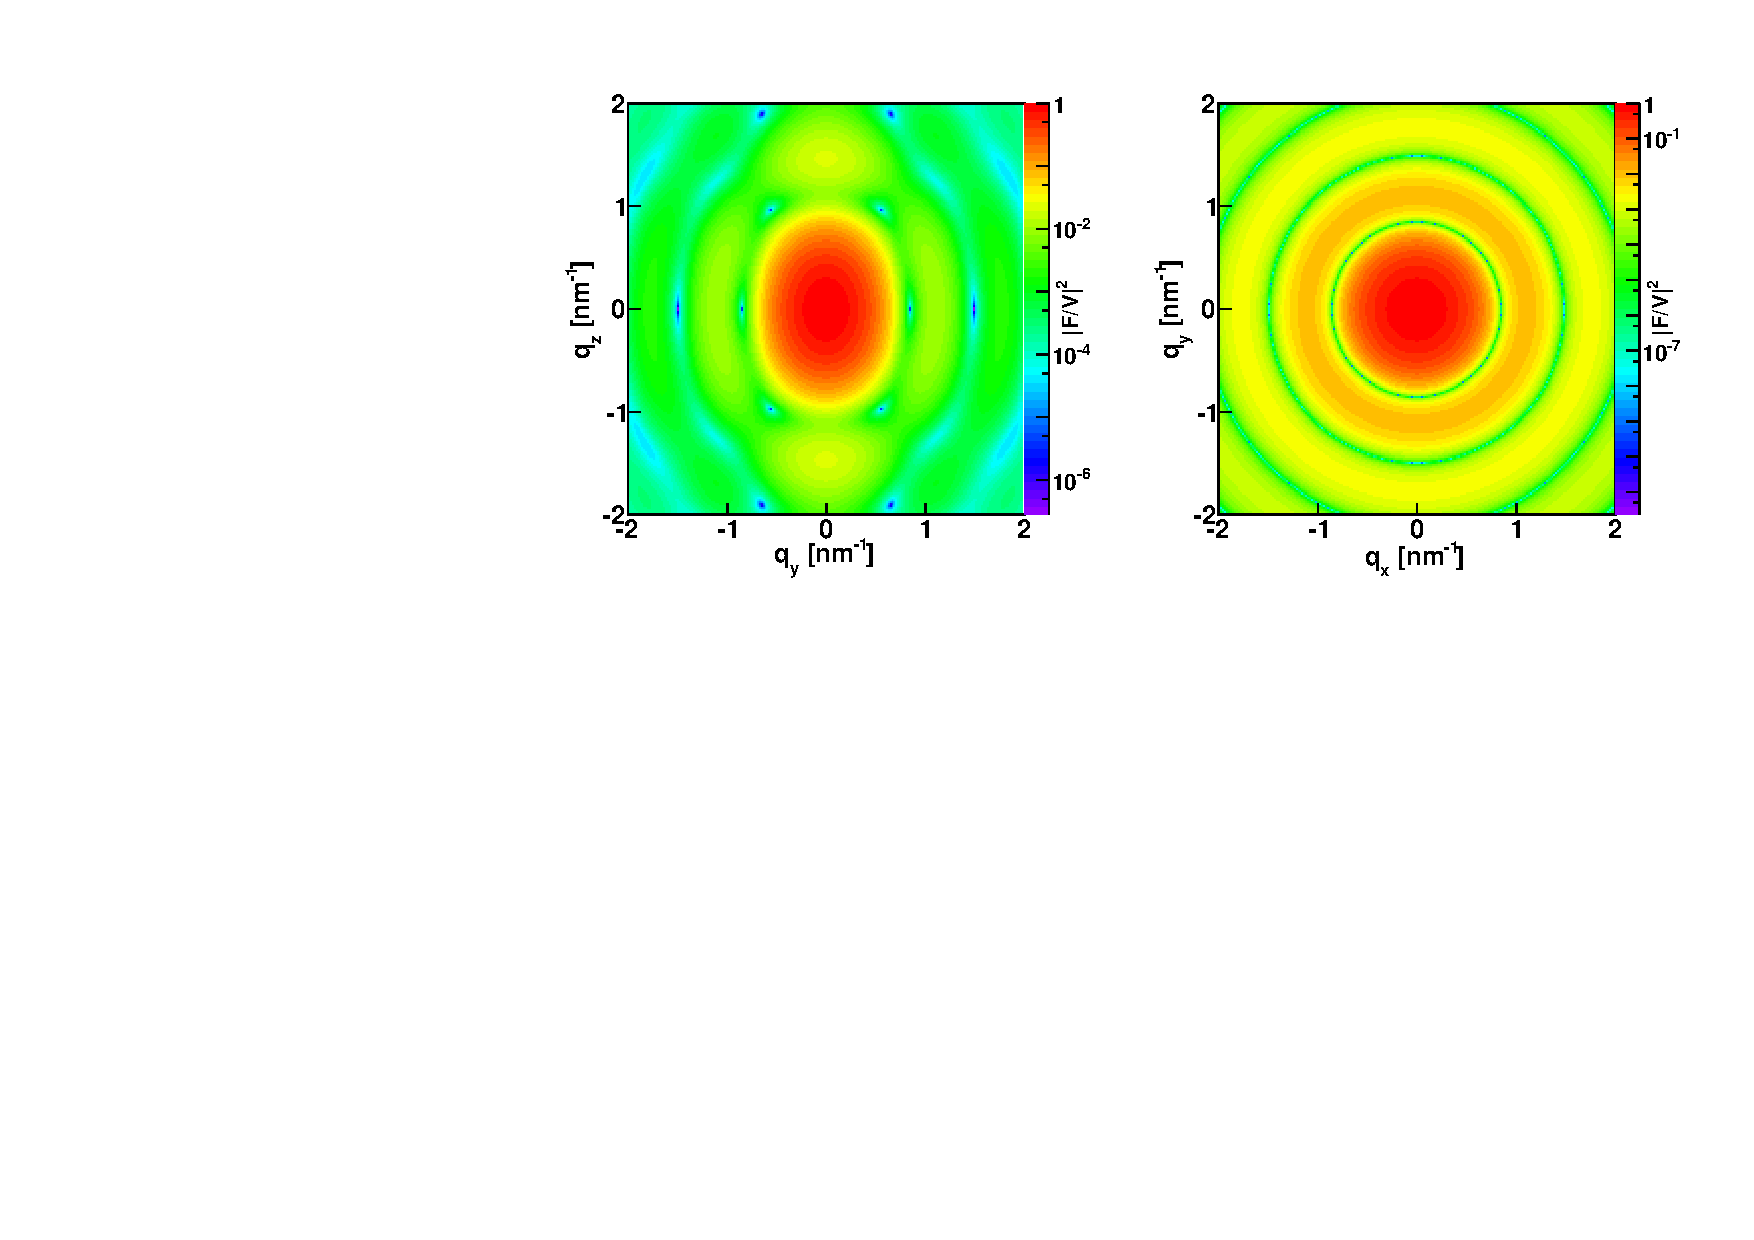
\includegraphics[width=0.9\textwidth]{Figures/figffsphere}
\end{center}
\caption{Computed results for $R=10$~nm and $H=13$~nm. {\bf a:} $|F|^2$ plotted against $q_z$ and $q_y$, {\bf b:} $|F|^2$ plotted against $q_x$ and $q_y$, {\bf c:} slice of the picture {\bf a} along the $q_z$ axis, {\bf d:} slice of the picture {\bf b} along the $q_x$ axis.}
\end{figure}

\par

\subsection{Parameter dependence}
Computed results for $R=10$~nm and $H=5$, 10 and 15~nm.
\begin{figure}[h]
\begin{center}
\includegraphics[width=0.9\textwidth]{Figures/ffspherepardep}
\end{center}
\caption{Computed results for $R=10$~nm and different values of $H$.}
\end{figure}


\subsection{Related particle shapes}
\begin{itemize}
\item Full sphere, \SecRef{FullSphere}
\item Ellipsoid
\item Full spheroid
\item Hemi-ellipsoid
\end{itemize} 

\subsection{References}

\newpage{\cleardoublepage}


\section{Formfactor Full Sphere}\SecLabel{FullSphere}
%\begin{lstlisting}[language=python, style=eclipseboxed,name=fffullsphere,nolol]
%from libBornAgainCore import * 
%fullsphere_ff = FormFactorFullSphere(5*nanometer)
%\end{lstlisting}
%\par
%~
%\par
Formfactor full sphere is represented as a sphere with radius $R$. 
\begin{figure}[ht]
\begin{center}
\includegraphics[width=0.6\columnwidth]{Figures/fullsphere}
\caption{Sketch of the formfactor full sphere. Left: front view, right: top view.}
\end{center}
\label{fullsphere}
\end{figure}

\begin{equation}
F(\mathbf q, R) = 4\pi R\times\frac{\sin(qR)-qR\cos(qR)}{(qR)^3}\times\exp\left(iq_zR\right)
\end{equation}

\begin{figure}[h]
\begin{center}
\includegraphics[width=0.9\textwidth]{Figures/figfffullsphere}
\end{center}
\caption{{\bf a:} $|F|^2$ plotted against $q_z$ and $q_y$, {\bf b:} $|F|^2$ plotted against $q_x$ and $q_y$, {\bf c:} slice of the picture {\bf a} along the $q_z$ axis, {\bf d:} slice of the picture {\bf b} along the $q_x$ axis.}
\end{figure}

\par


\chapter{User API} \label{UserAPI}

%%%%%%%%%%%%%%%%%%%%%%%%%%%%%%%%%%%%%%%%%%%%%%%%%%%%%%%%%%%%%%%%%%%%%%%%%%%%%%%%
\section{IntensityData}
%%%%%%%%%%%%%%%%%%%%%%%%%%%%%%%%%%%%%%%%%%%%%%%%%%%%%%%%%%%%%%%%%%%%%%%%%%%%%%%%

The \Code{IntensityData} object stores the 
simulated or real intensity data together with the axes definition of the detector in BornAgain's internal format. 
During the simulation setup
it is created automatically when the user specifies the detector characteristics and is filled with the simulated intensities after the simulation is completed.

\begin{lstlisting}[language=python, style=eclipseboxed]
simulation = Simulation()
simulation.setDetectorParameters(10, -5.0*degree, 5.0*degree, 5, 0.0*degree, 1.0*degree)
...
simulation.runSimulation()
intensity = simulation.getIntensityData() @\label{py:UserApi:intensity}@
\end{lstlisting}

The \Code{IntensityData} object retrieved in line~\ref{py:UserApi:intensity} corresponds to
the two dimensional detector pixel array as shown in Fig.~\ref{fig:UserApi:IntensityData}.

\begin{figure}[ht]
  \centering
    \includegraphics[clip=, width=120mm]{Figures/UserAPI_IntensityDataLayout.eps}
  \caption{The axes layout of IntensityData object.}
  \label{fig:UserApi:IntensityData}
\end{figure}

The x-axis and y-axis of the figure correspond to the $\phi_f$ and $\alpha_f$ axes of the detector. 
The x-axis is divided into 10 bins,
with low edge of the first bin set to $-5.0\,{\rm deg}$ and upper edge of the last bin set to $+5.0\,{\rm deg}$.
The y-axis is divided into 5 bins,
with low edge of the first bin set to $0.0\,{\rm deg}$ and upper edge of the last bin set to $1.0\,{\rm deg}$.
There are 50 bins in total (they are marked on the plot with indexes from 0 to 49), each bin will contain one intensity value.

During a standard simulation (i.e. no Monte-Carlo integration involved) intensities are calculated for $\phi_f, \alpha_f$ values corresponding to the bin centers, e.g. the intensity stored in bin\#42 will correspond to $\phi_f=3.5\,{\rm deg}, \alpha_f=0.5\,{\rm deg}$. 
\vspace*{2mm}


\MakeRemark{}{
The \Code{IntensityData} object is not intended for direct usage from Python API. The idea is 
that the API provides the user with the possibility to export the data from BornAgain internal format to the format of his choice as well as import user's data into BornAgain.
For the moment this functionality is limited to a few options explained below.
We encourage users feedback to implement the support of most requested formats.
}\\



\subsection{Import/export of intensity data}
For the moment we provide following options:
\begin{itemize}
\item Import/export of \Code{IntensityData} object from/to \Code{numpy} array.
\item Import/export of \Code{IntensityData} object from/to text file.

\end{itemize}

\subsubsection{Export to numpy array}

To export intensity data into  \Code{numpy} array the method \Code{getArray()} should be used 
on \Code{IntensityData} object as shown in line \ref{py:UserApi:getArray} of
following code snippet.

\begin{lstlisting}[language=python, style=eclipseboxed]
intensity = simulation.getIntensityData()
array = intensity.getArray() @\label{py:UserApi:getArray}@
...
pylab.imshow(numpy.rot90(array, 1)) @\label{py:UserApi:imshow}@
pylab.show()
\end{lstlisting}

For the detector settings defined in the previous paragraph the dimensions of the resulting array will be (10,5). By using \Code{numpy} indexes the user can get access to the intensity values, e.g.
\Code{array[0][0]} corresponds to the intensity in bin\#0 of Fig.~\ref{fig:UserApi:IntensityData},
\Code{array[0][4]} to bin\#4, 
\Code{array[1][0]} to bin\#5, 
\Code{array[8][2]} to bin\#42, 
\Code{array[9][4]} to bin\#49. 


To plot this resulting numpy array with \Code{matplotlib} it has to be rotated counter-clockwise
to match \Code{matplotlib} conventions as shown in line~\ref{py:UserApi:imshow}.


%\subsubsection{Direct access to the data}
%User can access to the

%\begin{lstlisting}[language=python, style=eclipseboxed]
%for i in range(0, intensity.getAllocatedSize()):
%    print intensity[i]
%\end{lstlisting}


\subsection{Importing from numpy array}

To use fitting the user has to load experimental data into BornAgain fitting kernel.
To read experimental data the user has to create
IntensityData object, fill it with the experimental  intensity values and pass
this object to the fitting kernel.

First, the user creates empty \Code{IntensityData} as shown
in line~\ref{py:UserApi:IntensityData} of the following code snippet.
\begin{lstlisting}[language=python, style=eclipseboxed]
data = IntensityData() @\label{py:UserApi:IntensityData}@
data.addAxis(FixedBinAxis("phi_f", 10, -5.0*degree, 5.0*degree)) @\label{py:UserApi:phi_f}@
data.addAxis(FixedBinAxis("alpha_f", 5, 0.0*degree, 1.0*degree)) @\label{py:UserApi:alpha_f}@
...
array = numpy.zeros((10, 5)) # fill array with experimental intensities @\label{py:UserApi:create_array}@
...
data.setRawDataVector(array.flatten().tolist()) @\label{py:UserApi:set_raw}@

fitSuite = FitSuite() @\label{py:UserApi:fit_suite}@
fitSuite.addSimulationAndRealData(simulation, data) @\label{py:UserApi:add_real_data}@
\end{lstlisting}

In lines~\ref{py:UserApi:phi_f}, \ref{py:UserApi:alpha_f} two axes with fixed bin sizes
are defined to represent the detector layout as shown in Fig.~\ref{fig:UserApi:IntensityData}. 
The constructor of \Code{FixedBinAxis} object has the following signature

\begin{lstlisting}[language=python, style=eclipse,numbers=none]
FixedBinAxis(title, nbins, min_angle, max_angle)
\end{lstlisting}

The created \Code{IntensityData} object has to be filled with experimental intensities
using \Code{numpy} array prepared by the user (lines ~\ref{py:UserApi:create_array}-~\ref{py:UserApi:set_raw}). In lines \ref{py:UserApi:fit_suite},\ref{py:UserApi:add_real_data} the fitting kernel is created and initialized with \Code{Simulation} object and 
\Code{IntensityData} object representing the experimental data.


\subsection{Saving intensity data to text file.}

The special class \Code{IntensityDataIOFactory} is intended for saving the intensity data
in different datafile formats. For the moment, it only supports saving the data in specific BornAgain's text files (the file extention \Code{*.int}).

\begin{lstlisting}[language=python, style=eclipseboxed]
intensity = simulation.getIntensityData()
IntensityDataIOFactory.writeIntensityData(intensity, 'file_name.int')
\end{lstlisting}

\subsection{Reading intensity data from a text file.}
The same class is also intended for reading intensity data
from files with different formats. For the moment, it only supports reading the data from text files of special BornAgain's format (the file extention \Code{*.int}).
 
\begin{lstlisting}[language=python, style=eclipseboxed]
intensity = IntensityDataIOFactory.readIntensityData('file_name.int')
\end{lstlisting}

%%\newpage
\chapter{\Python\ examples}
This appendix describes the samples and the simulated output intensity maps of the examples, whose \Python\ scripts are contained in the folder /Examples/python/simulation.

\section{General conventions}
\subsection{Geometry}

\begin{figure}[H]
\begin{center}
\includegraphics[width=0.6\textwidth]{Figures/BAgeometry_wide}
\end{center}
\caption{The GISAS setup and the coordinate system used in
\BornAgain. The incoming  beam propagates with incidence angles $\alpha_i$ and $\phi_i$ with respect to the sample axes as shown. A scattered (outgoing) beam, characterized by $\alpha_f$ and $\phi_f$ propagates toward the area detector.}
\label{fig:BAsetup_app}
\end{figure}


\begin{itemize}
\item The axis are defined on the interface of the sample with the air. 
The incoming beam points towards the positive $x$-axis direction. The $z$-axis points in the vertical upwards direction (see fig.~\ref{fig:BAsetup_app}).
\item The planes are assumed to be infinite in the planar direction $(x, y)$.
\item The substrate and the air layers are considered infinitely thick.
\item The scattered wave vector is defined as $\mathbf{q}=\mathbf{k}_i-\mathbf{k}_f$
\item The angles $\alpha_i$ and $\alpha_f$ are defined in such a way that those shown in fig.~\ref{fig:BAsetup_app}  are positive.
\item The refractive index of any material is defined as $n=1- \delta + i \beta$, where the values $\delta, \beta \in \mathbb R$ are the inputs used in \BornAgain.
\end{itemize}
Please refer to \SecRef{Simulation} for further details.

\subsection{Default settings}
By default the simulations with \BornAgain\ are performed using the Distorted Wave Born Approximation and the Decoupling Approximation regarding the spatial distribution of particles.


\subsection{Requirements}
\begin{itemize}
  \item The sample is built starting from the top layer.
  \item The particles are always associated with only one layer; they can be deposited on the top surface or buried in the layer. But they cannot cross interfaces.
\end{itemize}
The following sections describe some examples illustrating the main functionalities of \BornAgain .


\newpage
%%%%%%%%%%%%%%%%%%%%%%%%%%%%%%%
\section{Example 1: Cylinders and prisms}
The sample used in this example comprises a substrate on which are deposited, in equal proportion, cylinders and prisms (see fig.~\ref{fig:PythonEx1}(a)). All particles are made of the same material. Each type of particle has the same orientation.

The cylinders are 5~nm high and 5~nm in radius. The prisms are 5~nm high with a triangular base whose side length is equal to 10~nm (see \SecRef{Prism3} and \SecRef{Cylinder} for a description of these form factors). 

There is no interference between the waves scattered by these particles. The distribution is therefore diluted.

The incident neutron beam is characterized by a wavelength of 1~\AA, and incident angles $\alpha_i=0.2^{\circ}$ and $\phi_i=0^{\circ}$.

The simulation is performed using the Distorted Wave Born Approximation. The output intensity generated by this simulation is shown in fig.~\ref{fig:PythonEx1}(b).

\begin{figure}[H]
\hfill
\subfigure[Schematic of the sample]{\includegraphics[width=.49\textwidth]{Figures/fig_ex001}}
\hfill
\subfigure[Simulated 2D pattern]{\includegraphics[width=.49\textwidth]{Figures/figure_ex001.eps}}
\hfill
\caption{Example 1: equal proportion of cylinders and prisms3 deposited on a substrate without interference.}
\label{fig:PythonEx1}
\end{figure}

\newpage
%%%%%%%%%%%%%%%%%%%%%%%%%%%%%%%
\section{Example 2: Cylinders with size distribution} \SecLabel{AppPythonEx002}
Here the sample is made of polydisperse cylinders of two different sizes (see fig.~\ref{fig:PythonEx2}(a)). $R_1=H_1$, $R_2=H_2$, where $R_i$ and $H_i$ are the radius and width of cylinder of type $i$.  

There are 95\% of cylinders of type 1 and 5\% of cylinders of type 2.

The polydispersity affects the radii of the cylinders, following a normal distribution. For the small cylinder, their characteristic size varies about $R_1=5$~nm with a standard deviation $\sigma_1=0.2\ R_1$. For type 2, the average value $R_2$ is 10~nm and $\sigma_2=0.02\ R_2$. 

There is no substrate and no interference between the scattered beams.

The simulation is performed using the Born approximation, \textit{i.e.} the sample contains only "air" as a layer without any substrate.

The incident beam is characterized by a wavelength of 1~\AA and incident angles
$\alpha_i=0.2^{\circ}$ and $\phi_i=0^{\circ}$.

The result of the simulation is shown in fig.~\ref{fig:PythonEx2}(b). 

\begin{figure}[H]
\hfill
\subfigure[Schematic of the sample]{\includegraphics[width=.49\textwidth]{Figures/fig_ex002}}
\hfill
\subfigure[Simulated 2D pattern]{\includegraphics[width=.49\textwidth]{Figures/figure_ex002.eps}}
\hfill
\caption{Example 2: Polydisperse distribution of two types of cylinders.}
\label{fig:PythonEx2}
\end{figure}

\newpage
%%%%%%%%%%%%%%%%%%%%%%%%%%%%%%%
\section{Example 3: "Cylinder" form factor}
This example simulates cylindrical particles in three different configurations.
In each case the wavelength is equal to 1~\AA and the incident angles to $\alpha_i=0.2^{\circ}$, $\phi_i=0^{\circ}$. There is no interference between the scattered waves.

\subsection{Cylindrical form factor in Born approximation} \label{sec:ex003CylinderBA}
The sample considered for this example and the output intensity generated using \BornAgain\ are shown in fig.~\ref{fig:PythonEx3BA}(a) and (b), respectively. The cylinders are all identical with a radius and height equal to 5~nm. The simulation is performed in the Born approximation, by using only the air layer (no substrate).

\begin{figure}[H]
\hfill
\subfigure[Schematic of the sample]{\includegraphics[width=.49\textwidth]{Figures/fig_ex003BA}}
\hfill
\subfigure[Simulated 2D pattern]{\includegraphics[width=.49\textwidth]{Figures/figure_ex003BA.eps}}
\hfill
\caption{Example 3: Scattering from a monodisperse distribution of cylinders using the Born approximation.}
\label{fig:PythonEx3BA}
\end{figure}

\subsection{Cylindrical form factor in the Born approximation with size distribution}
This example considers a polydisperse distribution of cylinders (see fig.~\ref{fig:PythonEx3BASize}(a)). Their average radii and heights are equal to 5~nm. The radii of the cylinders vary according to a normal distribution with a standard deviation $\sigma$ equal to 0.2 times the average radius. The simulated output pattern is shown in fig.~\ref{fig:PythonEx3BASize}(b).

\begin{figure}[H]
\hfill
\subfigure[Schematic of the sample]{\includegraphics[width=.49\textwidth]{Figures/fig_ex003BASize}}
\hfill
\subfigure[Simulated 2D pattern]{\includegraphics[width=.49\textwidth]{Figures/figure_ex003BASize.eps}}
\hfill
\caption{Example 3: Scattering from a polydisperse distribution of cylinders using the Born approximation.}
\label{fig:PythonEx3BASize}
\end{figure}


\MakeRemark{Remark:}{ \\
This example differs from the one described in \SecRef{AppPythonEx002} by the presence of a single distribution of cylinders.}


\subsection{Cylindrical form factor in DWBA} \label{sec:ex003CylinderDWBA}
This example is similar to the case with  the Born Approximation (Section \ref{sec:ex003CylinderBA}) with the addition of a substrate (see fig.~\ref{fig:PythonEx3DWBA})(a)). Therefore the Distorted Wave Born Approximation is implemented in order to take additional reflections and transmission at the substrate interface into account.
The distribution of cylinders is monodisperse with a height and a radius of 5~nm.

\begin{figure}[H]
\hfill
\subfigure[Schematic of the sample]{\includegraphics[width=.49\textwidth]{Figures/fig_ex003DWBA}}
\hfill
\subfigure[Simulated 2D pattern]{\includegraphics[width=.49\textwidth]{Figures/figure_ex003DWBA.eps}}
\hfill
\caption{Example 3: Scattering from a monodisperse distribution of cylinders deposited on a substrate using the Distorted Wave Born approximation.}
\label{fig:PythonEx3DWBA}
\end{figure}

\newpage
%%%%%%%%%%%%%%%%%%%%%%%%%%%%%%%
\section{Example 4: Cylinders - Paracrystal}
The example focuses on the planar distribution of particles. Two cases are considered: a one- and a two-dimensional paracrystal. 
The two examples of this section share the following settings:
\begin{itemize}
\item The incident beam is characterized by a wavelength of 1~\AA and angles $\alpha_i=0.2^{\circ}$ and $\phi_i=0^{\circ}$.
\item The particles are cylinders with constant radii and heights equal to 5~nm. They are deposited on a substrate.
\end{itemize}

\subsection{"One dimension"}
The disorder is radially propagated. It is characterized by a Gaussian distribution $\exp(-\omega^2q^2/2)$ with $\omega=7$~nm.\\ The average distance between the particles $D$ is equal to  20~nm.\\ Finite size effects are modelled by introducing a damping length $\Gamma$ equal to 1e3~nm.\\
In this case, the structure factor is given by

\begin{equation*}
S(q_{\parallel})= \frac{1-\phi^2 }{1-2\phi\cos(q_{\parallel} D)+\phi^2} \; \textrm{with} \ \phi=\exp(-\omega^2 q_{\parallel}^2/2)\exp(-D/\Gamma).
\end{equation*}
%Its Fourier transform, the pair correlation function $g(r)$, is plotted in fig.~\ref{fig:PythonEx41DDL}a).


\begin{figure}[H]
\includegraphics[width=.49\textwidth]{Figures/figure_ex0041DDL.eps}
\caption{Example 4 - One dimension : Scattering from a distribution of cylinders deposited on a substrate using the Distorted Wave Born approximation, distribution according to a 1D paracrystal.}
\label{fig:PythonEx41DDL}
\end{figure}

%\begin{figure}[H]
%\hfill
%\subfigure[Pair distribution function as function of radial coordinate]{\includegraphics[width=.49\textwidth]{Figures/g_r_1dpara.eps}}
%\hfill
%\subfigure[Simulated 2D pattern]{\includegraphics[width=.49\textwidth]{Figures/figure_ex0041DDL.eps}}
%\hfill
%\caption{Example 4 - One dimension : Scattering from a distribution of cylinders deposited on a substrate using the Distorted Wave Born approximation, distribution according to a 1D paracrystal.}
%\label{fig:PythonEx41DDL}
%\end{figure}

\subsection{Two dimensions}
The cylindrical particles are distributed along a square lattice whose order is gradually distorted.
The average distance between the particles is 20~nm. The size of the domains is 20~$\mu$m in both directions.

The distribution function is a two-dimensional Cauchy function with correlation lengths equal to 1~nm in both directions.


\begin{figure}[H]
\hfill
\subfigure[Schematic of the sample]{\includegraphics[width=.49\textwidth]{Figures/g_r_2dparasq}}
\hfill
\subfigure[Simulated 2D pattern]{\includegraphics[width=.49\textwidth]{Figures/figure_ex0042DDLsq.eps}}
\hfill
\caption{Output ex004 2DDL.}
%\label{}
\end{figure}

\newpage
%%%%%%%%%%%%%%%%%%%%%%%%%%%%%%%
\section{Example 5: Lattice with disorder}
The examples of this section focus on the available options to characterize the pattern according to which the particles are deposited.


\subsection{Disorder 1} \label{sec:ex005Dis1}
Cylinders with radii and heights of 3~nm are deposited on a substrate (fig.~\ref{fig:PythonEx5Dis1}(a)). They are distributed along a square lattice with a lattice length of 25~nm, whose one of the main axes is parallel to the $x$-axis. The lattice is initialized by placing a cylinder at the origin.\\ The rod shape distribution is a two-dimensional Cauchy function in reciprocal space with anisotropic correlation lengths equal to $cl_x=300/(2\pi)$~nm and $cl_y=100/(2\pi)$~nm.
%The probability distribution function is a two-dimensional Cauchy function  with anisotropic correlation lengths equal to $cl_x=300/(2\pi)$~nm and $cl_y=100/(2\pi)$~nm.


The incident beam is characterized by a wavelength of 1~\AA and angles $\alpha_i=0.2^{\circ}$ and $\phi_i=0^{\circ}$.
 
The simulation is run using the DWBA.

% question: LMA with constant size of particles?? 
\begin{figure}[H]
\hfill
\subfigure[Schematic of the sample]{\includegraphics[width=.49\textwidth]{Figures/fig_ex005Dis1}}
\hfill
\subfigure[Simulated 2D pattern]{\includegraphics[width=.49\textwidth]{Figures/figure_ex005Disorder1.eps}}
\hfill
\caption{Example 005 - Disorder1: Scattering from a monodisperse distribution of cylinders deposited on a substrate along a squared lattice using the Distorted Wave Born approximation.}
\label{fig:PythonEx5Dis1} 
\end{figure}

\subsection{Disorder 2}
This sample differs from the previous one by an overlap of two spatial distributions of cylinders. The first square lattice is centered at the origin. The second one, with the same lattice spacing and the same cylinders at the nodes is initialized at $x=y=12.5$~nm.

\begin{figure}[H]
\hfill
\subfigure[Schematic of the sample]{\includegraphics[width=.49\textwidth]{Figures/fig_ex005Dis2}}
\hfill
\subfigure[Simulated 2D pattern]{\includegraphics[width=.49\textwidth]{Figures/figure_ex005Disorder2.eps}}
\hfill
\caption{Example 005 - Disorder2: Scattering from two monodisperse distributions of cylinders deposited on a substrate along a squared lattice using the Distorted Wave Born approximation. One of the lattices is laterally offset with respect to the other by 12.5~nm along the $x-$ and $y-$ axes.}
\label{fig:PythonEx5Dis2} 
\end{figure}

\subsection{Disorder 3}
Compared to Section~\ref{sec:ex005Dis1}, the square lattice used in this example is now rotated with respect to the main referential by $30^{\circ}$. Note that the axes of the rod shape's distribution are also rotated using \Code{setGamma}.



\begin{figure}[H]
\hfill
\subfigure[Schematic of the sample]{\includegraphics[width=.49\textwidth]{Figures/fig_ex005Dis3}}
\hfill
\subfigure[Simulated 2D pattern]{\includegraphics[width=.49\textwidth]{Figures/figure_ex005Disorder3.eps}}
\hfill
\caption{Example 005 - Disorder3: Scattering from a monodisperse distribution of cylinders deposited on a substrate along a squared lattice using the Distorted Wave Born approximation. The main axes of the square lattice are rotated by 30$^{\circ}$ with respect to the main referential.}
\label{fig:PythonEx5Dis3}
\end{figure}


\subsection{Disorder 4}
This sample is composed of identical cylinders. Their distribution is generated as a random subset of three rotated square lattices (their main axes are rotated with respect to the $x$-axis by  0$^{\circ}$, $120^{\circ}$, $240^{\circ}$, respectively).

\begin{figure}[H]
\hfill
\subfigure[Schematic of the sample]{\includegraphics[width=.49\textwidth]{Figures/fig_ex005Dis4rand}}
\hfill
\subfigure[Simulated 2D pattern]{\includegraphics[width=.49\textwidth]{Figures/figure_ex005Disorder4.eps}}
\hfill
\caption{Example 005 - Disorder4: Scattering from a monodisperse distribution of cylinders deposited on a substrate.}
\label{fig:PythonEx5Dis4}
\end{figure}

\newpage
%%%%%%%%%%%%%%%%%%%%%%%%%%%%%%%
\section{Example 6: Rotated pyramids}
This example illustrates how the in-plane rotation of non-radially symmetric particles influences the scattering pattern. \\
The sample is made of pyramids (squared-base side length = 10~nm, height = 5~nm, $\alpha=54.73^{\circ}$, see \SecRef{Pyramid}) deposited on a substrate. There is no interference.\\
The wavelength is 1~\AA. The incident angles are $\alpha_i=0.2^{\circ}$ and $\phi_i=0^{\circ}$.\\
For the second example, shown in fig.~\ref{fig:PythonEx6RotatedPyramid}, the pyramids are rotated in the $(x,y)$ plane by 45$^{\circ}$.

\begin{figure}[H]
\hfill
\subfigure[Schematic of the sample]{\includegraphics[width=.49\textwidth]{Figures/fig_ex006Pyramids}}
\hfill
\subfigure[Simulated 2D pattern]{\includegraphics[width=.49\textwidth]{Figures/figure_ex006Pyramids.eps}}
\hfill
\caption{Example 6: Pyramids deposited on a substrate.}
\label{fig:PythonEx6Pyramid}
\end{figure}

\begin{figure}[H]
\hfill
\subfigure[Schematic of the sample]{\includegraphics[width=.49\textwidth]{Figures/fig_ex006RotatedPyramids}}
\hfill
\subfigure[Simulated 2D pattern]{\includegraphics[width=.49\textwidth]{Figures/figure_ex006RotatedPyramids.eps}}
\hfill
\caption{Example 6: Rotated pyramids deposited on a substrate.}
\label{fig:PythonEx6RotatedPyramid}
\end{figure}

\newpage
%%%%%%%%%%%%%%%%%%%%%%%%%%%%%%%
\section{Example 7: Core-shell nanoparticles}
The sample is made of core-shell particles whose inner and outer shells are parallelepipeds with dimensions  $L_1=W_1=16$~nm, $H_1=8$~nm and  $L_2=W_2=12$~nm, $H_2=7$~nm, respectively, where $L_i$, $W_i$, and $H_i$ are the length, width and height of box $i$ (see fig.~\ref{fig:PythonEx7Core}). The smaller box is positioned so that the centres of the bottom faces of both particles coincide (see \ref{subsec:CoreShell} for details about this form factor). 

The simulation is run using the Born approximation. There is no substrate and no interference between the different scattered beams.

The incident beam is characterized by a wavelength of 1~\AA, incident angles $\alpha_i=0.2^{\circ}$ and $\phi_i=0^{\circ}$.


\begin{figure}[H]
\hfill
\subfigure[Schematic of the sample]{\includegraphics[width=.49\textwidth]{Figures/fig_ex007Core}}
\hfill
\subfigure[Simulated 2D pattern]{\includegraphics[width=.49\textwidth]{Figures/figure_ex007CoreShell.eps}}
\hfill
\caption{Example 7: Core-shell particles simulated using the Born approximation. The particle at the forefront had been truncated in order to illustrate the core-shell structure.}
\label{fig:PythonEx7Core}
\end{figure}

\newpage
%%%%%%%%%%%%%%%%%%%%%%%%%%%%%%%
\section{Example 8: Correlated roughness}
The sample is made in the following way from top to bottom: 

\begin{itemize}
    \item \ntikzmark{L}{layer A: A: 2.5~nm-thick, $n=1-5e-6$.}
    \item \ntikzmark{O}{layer B:  5~nm-thick, $n=1-1e-5$.}
    \item substrate: infinitely thick, $n=1-15e-6$
\end{itemize}
\makebrace{L}{O}{$\times$ 5.}

There is no added particle. All layers present the same type of roughness on the top surface, which is characterized by
\begin{itemize}
\item $\sigma=1$~nm,
\item a Hurst parameter $H$ equal to 0.3,
\item a lateral correlation length $\xi$ of 5~nm,
\item a cross correlation length $\xi_{\perp}$ equal to 1e-4~nm.
\end{itemize}

\MakeRemark{Roughness in \BornAgain}{The implementation is based on Reference~\cite{Boer95,Schlomka95}.\\ The roughness profile is described by a normally-distributed random function. The roughness correlation function at j$^\textrm{th}$ interface is expressed as  $\langle U_j(x,y) U_j(x',y') \rangle = \sigma^2 \exp(-(\tau/\xi)^{2H})$,
 $\tau=\sqrt{(x-x')^2+(y-y')^2}$, where $U_j(x,y)$ is the height deviation of the j$^{\textrm{th}}$ interface at position $(x,y)$.
\\ $\sigma$ gives the rms roughness of the interface.\\ The Hurst parameter $H$, comprised between 0 and 1 is connected to the fractal dimension $D=3-H$ of the interface. The smaller $H$ is, the more serrate the surface profile looks. If $H=1$, the interface has a non fractal nature.\\ The lateral correlation length $\xi$ acts as a cut-off for the lateral length scale on which an interface begins to look smooth. If $\xi >> \tau$ the surface looks smooth.\\ The cross correlation length $\xi_{\perp}$ is the vertical distance over which the correlation between layers is damped by a factor $1/e$. It is assumed to be the same for all interfaces. If $\xi_{\perp}=0$ there is no correlations between layers. If $\xi_{\perp}$ is much larger than the layer thickness, the layers are perfectly correlated.}

The incident beam is characterized by a wavelength of 1~\AA \ and incident angles $\alpha_i=0.2^{\circ}$ and $\phi_i=0^{\circ}$. 
\begin{figure}[H]
\hfill
\subfigure[Schematic of the sample]{\includegraphics[width=.49\textwidth]{Figures/fig_ex008Rough}}
\hfill
\subfigure[Simulated 2D pattern]{\includegraphics[width=.49\textwidth]{Figures/figure_ex008CorrelatedRough.eps}}
\hfill
\caption{Example 8: Correlated roughness between layers.}
\label{fig:PythonEx8Rough}
\end{figure}

%Power spectral density of the surface roughness is a result of two-dimensional
%Fourier transform of the correlation function of the roughness profile.
% Based on the article D.K.G. de Boer, Physical review B, Volume 51, Number 8, 15 February 1995 "X-ray reflection and transmission by rough surfaces"
 
\newpage
%%%%%%%%%%%%%%%%%%%%%%%%%%%%%%%
\section{Example 9: Ripple}
These particles have one of their dimensions much larger than the others.
Two different transverse profiles are simulated: one cosine and one asymmetric triangular.
These particles are deposited on a substrate. The input beam is characterized by a wavelength of 1.6~\AA and angles $\alpha_i=0.3^{\circ}$, $\phi_i=0^{\circ}$.

\subsection{Cosine ripple}
The particles have a cosine cross section (see \SecRef{Ripple1} for an illustration) with $L=100$~nm, $W=20$~nm, $H=4$~nm.
The interference considered is a two-dimensional orthogonal lattice with $L_1=200$~nm, $L_2=50$~nm. The rod shape distribution is an anisotropic 2D Gaussian with $cl_x=1000/(2\pi)$~nm and  $cl_y=100/(2\pi)$~nm.

\begin{figure}[H]
\hfill
\subfigure[Schematic of the sample]{\includegraphics[width=.49\textwidth]{Figures/fig_ex009Cos}}
\hfill
\subfigure[Simulated 2D pattern]{\includegraphics[width=.49\textwidth]{Figures/figure_ex009CosRipple2DLat.eps}}
\hfill
\caption{Example 9: Scattering from a distribution of cosine ripples deposited on a substrate along a rectangular lattice.}
\label{fig:PythonEx9CosRipple}
\end{figure}

The influence of the interference function on the output pattern can be seen by comparing figures~\ref{fig:PythonEx9CosRipple}(b) and \ref{fig:PythonEx9CosRipplenointerf}. The latter has been generated without any interference (\textit{i.e.} with a diluted distribution of particles).

\begin{figure}[H]
\begin{center}
\includegraphics[width=0.5\textwidth]{Figures/figure_ex009CosRippleNoInterf.eps}
\end{center}
\caption{Example 9: Scattering from a distribution of cosine ripples deposited on a substrate with no interference.}
\label{fig:PythonEx9CosRipplenointerf}
\end{figure}

\subsection{Triangular ripple}
 The particles are long particles with an asymmetric triangular cross section (see \SecRef{Ripple2}) with  $L=100$~nm, $W=20$~nm, $H=4$~nm, an asymmetry coefficent of $-3$~nm. The interference function has the same characteristics as in the previous example.

\begin{figure}[H]
\hfill
\subfigure[Schematic of the sample]{\includegraphics[width=.49\textwidth]{Figures/fig_ex009Tri}}
\hfill
\subfigure[Simulated 2D pattern]{\includegraphics[width=.49\textwidth]{Figures/figure_ex009TriRipple2DLat.eps}}
\hfill
\caption{Example 9: Scattering from a distribution of triangular ripples deposited on a substrate with no interference.}
\label{fig:PythonEx9TriangRipple}
\end{figure}

Figure~\ref{fig:PythonEx9TriRipplenointerf} was generated with asymmetrical triangular ripples but with no interference. It therefore illustrates the influence of the particle's shape on the scattering pattern.

\begin{figure}[H]
\begin{center}
\includegraphics[width=0.5\textwidth]{Figures/figure_ex009TriRippleNoInterf.eps}
\end{center}
\caption{Example 9: Scattering from a distribution of triangular ripples deposited on a substrate with no interference.}
\label{fig:PythonEx9TriRipplenointerf}
\end{figure}

\newpage
%%%%%%%%%%%%%%%%%%%%%%%%%%%%%%%
\section{Example 10: Beam divergence}
The main point of this example is the input beam, which presents a divergence for:
\begin{itemize}
\item the wavelength, following a log-normal distribution around the mean value of 1~\AA\ with a scale parameter equal to 0.1 (see the remark at the end of this section for a definition of these parameters).
\item  both incident angles following a Gaussian distribution with 
$\bar \alpha_i=0.2^{\circ}$, $\bar\phi_i=0^{\circ}$ and $\sigma_{\alpha_i}=\sigma_{\phi_i}=0.1^{\circ}$.
\end{itemize}
The sample is made of cylinders (5~nm in radius and height) deposited on a substrate, whose scattered beams do not interfere (fig.~\ref{fig:PythonEx10BeamDiv}(a)). The simulation is run using the Distorted Wave Born Approximation.

\begin{figure}[H]
\hfill
\subfigure[Schematic of the sample]{\includegraphics[width=.49\textwidth]{Figures/fig_ex010BeamDiv}}
\hfill
\subfigure[Simulated 2D pattern]{\includegraphics[width=.49\textwidth]{Figures/figure_ex010BeamDiv.eps}}
\hfill
\caption{Example 10: An input beam presented a divergence for the wavelength and the incident angles impinges on a sample made of monodisperse cylinders deposited on a substrate.}
\label{fig:PythonEx10BeamDiv}
\end{figure}

This example and the one presented in Section~\ref{sec:ex003CylinderDWBA} differ only by the divergence of the input beam. Comparing the output patterns shows that the largest impact of input beam divergence is a reduction of the sharpness in the intensity pattern for larger values of $\phi_f$ and $\alpha_f$.\\



\MakeRemark{Remark:}{The Gaussian distribution is characterised by 
$$p(\bar{x},\sigma)=\frac{1}{2\sigma^2}\exp\left[-\frac{(x-\bar{x})^2}{2\sigma^2} \right], $$
and the log-normal by
$$p(\textrm{median}, \textrm{scale})=\frac{1}{x\ \textrm{scale}\sqrt{2\pi}}\exp\left[-\frac{1}{2}\left( \frac{\log(x/\textrm{median})}{\textrm{scale}} \right)^2 \right].$$
}




\bibliographystyle{switch}
\bibliography{jw7}
\end{document}
